\documentclass[aps,floatfix,showpacs,preprintnumbers,twocolumn,nofootinbib]{revtex4}


%\biboptions{sort&compress}
\usepackage{hyperref}
\usepackage{amssymb}
\usepackage{amsfonts}
\usepackage{amsmath}
\usepackage{graphicx}
\usepackage{dcolumn}
\usepackage{mathrsfs}
\usepackage{bigints}
\usepackage{bm}
\usepackage{natbib}
\usepackage{color}
\usepackage{lscape}
\usepackage{epstopdf}
\epstopdfsetup{update}
\DeclareGraphicsExtensions{.ps}
\epstopdfDeclareGraphicsRule{.ps}{pdf}{.pdf}{ps2pdf -dEPSCrop -dNOSAFER #1 \OutputFile}
\DeclareGraphicsExtensions{.jpg.ps}
\epstopdfDeclareGraphicsRule{.jpg.ps}{pdf}{.pdf}{ps2pdf -dEPSCrop -dNOSAFER #1 \OutputFile}

\graphicspath{{figs/}}

\def\RCG#1{{\color{red}#1}}
\newcommand{\sslash}{\mathbin{/\mkern-4mu/}}

\def\sn{{\rm sn}}
\def\cn{{\rm cn}}
\def\csch{{\rm csch}}


\begin{document}
%\baselineskip 14.5pt

\title{On the temporal tweezing of cavity solitons}
%
\author{J. Rossi$^{1}$, R. Carretero-Gonz\'{a}lez$^{1,}$\footnote{{\tt URL:} http://www.rohan.sdsu.edu/$\sim$rcarrete/}, and P. G. Kevrekidis$^{2}$.  }
\affiliation{
$^{1}$Nonlinear Dynamical Systems Group\footnote{{\tt URL:} http://nlds.sdsu.edu/}
Computational Science Research Center\footnote{{\tt URL:} http://www.csrc.sdsu.edu/}, and
Department of Mathematics and Statistics,
San Diego State University, San Diego, California 92182-7720, USA
\\
$^{2}$Department of Mathematics and Statistics, University of Massachusetts, Amherst, Massachusetts 01003-4515, USA%
}
\date{\today}

\begin{abstract}
We explore the non-conservative variational approximation (NCVA) formulation for complex partial differential equations of the nonlinear Schr\"{o}dinger (NLS) type, using Galley's~[Phys.~Rev.~Lett.~{\bf 110}, 174301 (2013)] proposed initial value problem formulation of Hamilton's principle for non-conservative systems.  We study a variant of the NLS used in optical systems called the Lugiato-Lefever (LL) model applied to temporal tweezing of cavity solitons in a passive loop of optical fiber pumped by a continuous-wave laser beam observed experimentally by Jang, Erkintalo, Coen, and Murdoch in Nat.~Commun.~{\bf 6}, 7370 (2015).  We study the existence and dynamics of cavity solitons through phase-modulation of the holding beam.  We find parametric regions for the manipulation of cavity solitons by a tweezer in the LL model.  We also explore the ability of the NCVA method at capturing the evolution of solitary waves.
%
\end{abstract}

\pacs{}
\maketitle


%%%%%%%%%% Section: Introduction
\section{Introduction}
An optical tweezer, i.e.,~a single-beam gradient force trap, can trap, manipulate and move nanometer and micron-sized dielectric particles in space using a highly focused laser beam~\cite{Ashkin1970,Ashkin1986}.  Optical tweezers have been used in physics and biology to manipulate objects and measure forces~\cite{ChuOpt}.  Comparatively, a temporal tweezer can exert similar control over ultrashort light pulses in time, as observed by Jang, Erkintalo, Coen, and Murdoch in Ref.~\cite{tweeze}.  The optical trapping and manipulation of light pulses is useful in optical information processing~\cite{info1, info2, info3, info4}, in which the information is represented as a sequence of pulses.  Therefore, temporal tweezing is an effective method to trap ultrashort pulses of light and move them around in {\em time} in order to store and reconfigure the information.  Optical information processing is partly achieved in slow-light~\cite{info5, info6, info7, info8} and nonlinear cross-phase modulation effects~\cite{info9, info10, info11, info12, info13, info14}, however neither approach allows for the independent control of light pulses within the sequence.  
Based on Ref.~\cite{tweeze}, we present an exhaustive numerical analysis of temporal tweezing as well as its non-conservative variational approach (NCVA) reduction.  
%

We investigate temporal tweezing of cavity solitons in a passive loop of optical fiber pumped by a continuous-wave laser beam which is described by a modified LL model.  The optical trapping and manipulation of the temporal position of light pulses is highly desirable as it has immediate implications for optical information processing which has recently been realized experimentally~\cite{tweeze}.  Information is treated as a sequence of pulses that can be stored and reconfigured by trapping ultrashort pulses of light and dynamically moving them around in time.  In the experiment, temporal cavity solitons (CSs) exist as picosecond pulses of light that recirculate in a loop of optical fibre and are exposed to temporal controls in the form of a gigahertz phase modulation.  It has been shown, both theoretically and experimentally, that the CSs are attracted and trapped to phase maxima, suppressing all soliton interactions.  These trapped CSs can then be manipulated in time, either forward or backward, which is known as temporal tweezing.  We study the existence and dynamics of temporally tweezed CSs.  The key phenomena reported herein are parametric intervals for the existence of tweezed CSs, dissipative CSs, and non-tweezed CSs.  We also apply the NCVA to identify regions of temporal tweezing, and compare to the full numerical solutions of the original PDE.    
%

The paper is organized as follows.  
%
In Sec~\ref{section:TTweeze} we introduce the temporal tweezing approach suggested in Ref.~\cite{tweeze} and setup of the Lugiato-Lefever (LL) model.  
%
In Sec.~\ref{section:TweezePDE} we add a gaussian phase-modulation to the LL model and simulate the moving and manipulation of the cavity soliton (CS).  
%
In Sec.~\ref{secNCVA:prelim} we provide a brief description of the NCVA approach and its formulation within the LL model.  Section~\ref{section:TweezeNCVA} is devoted to the application of the NCVA to capture the tweezing of a CS.  
%
In Sec.~\ref{section:TweezeResults} we identity the existence and dynamics of trapped cavity solitons manipulated through phase-modulation of a continuous-wave holding beam.  Finally, in Sec~\ref{secConclusion} we summarize our key findings and we provide possible avenues for future research.


%%%%%%%%%% Section LLE Model + Modulation
\section{The Full Model: Lugiato-Lefever Equation and Temporal Phase Modulation
\label{section:TTweeze}}
In our analysis of temporal tweezing we begin with dissipative solitons in externally-driven nonlinear passive cavities called temporal CSs~\cite{XuCoenRef22a,XuCoenRef22b,info15,info17,info19,info21}.  In a passive loop of optical fiber these pulses of light can persist without losing shape because the dispersive temporal spreading is balanced by the material nonlinearity.   Also, CSs persist without losing their intensity by drawing power from a continuous-wave (cw) ``holding'' laser beam driving the cavity.  Multiple CSs may be simultaneously present in the optical loop and position independently temporally~\cite{info16}.  Here, we report on the trapping of CSs and the dynamical manipulation through selectively altering the phase profile of the holding beam.  

\subsection{Theory of Temporal Tweezing}  
\label{secTweezeTheroy}

Temporal tweezing requires a CS with an attractive time-domain drift towards the maxima of the intracavity phase profile.  The attraction is due to the CSs shifting their instantaneous frequencies in reaction to a phase modulation.   This system is modeled by the mean-filed Lugiato-Lefever equation (LL)~\cite{tweeze,LL,LLE},
\begin{align}
z_R \frac{\partial E }{\partial z} = \left[ -\alpha - i \delta_0 - i L \frac{\beta_2}{2} \frac{\partial^2}{\partial \tau^2} + i \gamma L |E|^2 \right] E + \sqrt{\theta}E_{\mathrm{in}},
\label{eq:LLETweeze1}
\end{align}
where $z$ is the slow time describing the intracavity field envelope $E(z,\tau)$ over subsequent cavity roundtrips and $\tau$ is the fast time describing the temporal profile of the field envelope in a reference frame traveling at the group velocity of the holding beam in the cavity.  The cavity roundtrip time is $z_R$.  The field of the holding beam is $E_{\mathrm{in}}$ with power $P_{\mathrm{in}} = |E_{\mathrm{in}}|^2$.  The cavity losses are accounted for in $\alpha = \pi/\mathscr{F}$, with cavity finesse $\mathscr{F}$.  The phase detuning of the intracavity field to the closest cavity resonance of order $l$ is given by $\delta_0 = 2\pi l - \phi_0$ where $\phi_0$ is a linear phase-shift over one roundtrip with respect to the holding beam.  $L$ is the cavity length, $\beta_2$ is the dispersion coefficient of the fibre, $\gamma$ is the nonlinear coefficient of the fibre, and finally $\theta$ is the input coupler power transmission coefficient.  

The LL Eq.~(\ref{eq:LLETweeze1}) may be adimensionalized in order to be less cumbersome by introducing a dimensionless slow time $z' = \alpha z / z_R$ and a dimensionless fast time $\tau' = \tau \sqrt{2\alpha /(L |\beta_2|)}$.  We also use a dimensionless complex filed amplitude $v(z',\tau') = E(z,\tau) \sqrt{\gamma L/\alpha}$ and a dimensionless holding beam $v_{\mathrm{in}} = E_{\mathrm{in}}\sqrt{\gamma L \theta /\alpha^3}$.  For convenience, we drop the primes in the notation of $z'$ and $\tau'$, such that Eq.~(\ref{eq:LLETweeze1}) becomes the dimensionless mean-field Lugiato-Lefever equation 
\begin{align}
\frac{\partial v }{\partial z} = -(1+i \Delta) v + i |v|^2 v + i \frac{\partial^2 v }{\partial \tau^2} + v_{\mathrm{in}},
\label{eq:dimensionlessLLE}
\end{align}
where $\Delta = \delta/\alpha$ is the effective dimensionless detuning.  

The homogeneous steady states of Eq.~(\ref{eq:dimensionlessLLE}) satisfy 
\begin{align}
|v|^2 v = -i v + \Delta v+ i v_{\mathrm{in}}, 
\label{steadyStateNLS}
\end{align}
which may be cast in the form of a well-known cubic equation for dispersive optical bistability~\cite{Grelu,LL,info2,Gomila2007}
\begin{align}
I_s^3 - 2\Delta I_s^2 + (1+ \Delta) I_s = I_0,
\label{steadystate2}
\end{align}
where $I_s = |v_s|^2$ is the intracavity field intensity and $I_0 = |v_{\mathrm{in}}|^2$ is the holding beam intensity.  Therefore, we obtain a steady state solution
\begin{align}
v_s = \frac{v_{\mathrm{in}}}{1+ i (\Delta - I_s)},
\end{align}
dependent on the detuning $\Delta$ and holding beam power $v_{\mathrm{in}}$.  For small detuning, $\Delta < \sqrt{3}$, Eq.~(\ref{steadystate2}) has only one solution for the the steady state $I_s$ given a specific holding beam power $v_{\mathrm{in}}$.  For detuning, $\Delta > \sqrt{3}$ there are three solutions for $I_s$ given a specific holding beam power $v_{\mathrm{in}}$.  The homogeneous solution is bistable since two solutions are stable while the other solution is unstable.  The transition between the states occurs through a pitchfork bifurcation.

We follow the approach of Refs.~\cite{tweeze,firth96} to study the effect of phase-modulation of the holding field.  The phase-modulation is imprinted into a constant holding beam which creates an effective potential necessary to attract, trap, and manipulate a CS.  We assume a phase-modulation temporal profile $\phi(\tau)$.  We rewrite the holding beam using  
\begin{align}
v_{\mathrm{in}} (\tau) = u_{\mathrm{in}} \exp[i \phi(\tau)], \label{uin}
\end{align}
where $u_{\mathrm{in}}$ is a constant scalar.  Substituting Eq.~(\ref{uin}) into Eq.~(\ref{eq:dimensionlessLLE}) with the ansatz $v(z, \tau) = u(z, \tau) \exp[i \phi(\tau)]$ yields 
\begin{align}
i u_z + |u|^2 u + u_{\tau\tau} -& (\Delta + (\phi')^2) u + 2i u_{\tau} \phi' = \nonumber \\
& - i (1+\phi'') u + i u_{\mathrm{in}}.
\label{eq:LLETweeze}
\end{align}
The cw intracavity field on which the CSs are superimposed still has the same phase modulation as that imposed on the external holding beam in this nondimensional form.  In this form, $(\phi')^2$ acts like an effective potential caused by the phase modulation while $ 2i u_{\tau} \phi'$ is the effect of drift through the gradient term $u_{\tau}$ where $2 \phi'$ is the drift speed~\cite{ParraRivas2014}.  The $\phi''$ term induces an additional loss in the system caused by the phase modulation.

Steady state solutions of the LL Eq.~(\ref{eq:LLETweeze}) are subject to an additional constraint stemming from the balance condition $dP/dz= 0$, where 
\begin{align}
P \equiv \int_{-\infty}^{\infty} |u|^2 d \tau,
\end{align}
is the total power of the cavity solitons (mathematically the squared $L^2$ norm).  The evolution of $P$ can be found by multiplying Eq.~(\ref{eq:LLETweeze}) by $u^*$, the complex conjugate of Eq.~(\ref{eq:LLETweeze}) by $u$, and then adding and integrating the resulting equations as shown in~\cite{Theocharis2006}.  For the LL Eq.~(\ref{eq:LLETweeze}), it is straightforward to find the following constraint condition for a steady state solution:
\begin{align}
\int_{-\infty}^{\infty} \Big( - (1 + \phi'') |u|^2 - \phi' \left(u_{\tau} u^* + u_{\tau}^* u \right) +\nonumber \\
 \frac{1}{2} (u^* + u ) u_{\mathrm{in}} \Big) d \tau = 0,
\label{LLConstraint}
\end{align} 
which can be further simplified using $\frac{1}{2} (u^* + u ) = \mathrm{Re} (u)$.  This power-balance constraint will need to be enforced in the system, and in turn, will fix the cavity detuning $\Delta$ for a given set of parameters describing $\phi$. 

\subsection{Tweezability of Cavity Solitons} 
\label{section:TweezePDE}
Our analysis involves temporal cavity solitons described by LL Eq.~(\ref{eq:LLETweeze}) stored in a passive loop of optical fiber pumped by a cw laser beam.  The CS is trapped into a specific time slot through phase-modulation of the holding beam, and moved around in time by manipulating the phase profile.  Experimentally, a modulator imprints a time-varying electric signal $\phi(\tau)$ into the phase of a the cw holding laser driving the cavity.  For the purpose of the LL Eq.~(\ref{eq:LLETweeze}), we used a ``natural'' Gaussian phase profile of the form
\begin{align}
\phi(\tau) = h_{\phi} \exp\left[ -\frac{(\tau - \tau_0)^2}{2 \sigma_{\phi}^2} \right],
\label{phi}
\end{align}
where $h_{\phi}$, $\sigma_{\phi}$, and $\tau_0$ represent, respectively, the height, width, and center position of the phase profile.  For the LL model, the first and second derivative of the phase profile are, respectively, 
\begin{align}
\phi' &= \frac{d \phi}{d \tau} = -\frac{h_{\phi} ( \tau - \tau_0)}{\sigma_{\phi}^2} e^{\left( -\frac{(\tau - \tau_0)^2}{2 \sigma_{\phi}^2}  \right)}\label{firstphi}, \\
\phi'' &= \frac{d^2 \phi}{d \tau^2} = -\frac{h_{\phi} }{\sigma_{\phi}^2} e^{ \left[ -\frac{(\tau - \tau_0)^2}{2 \sigma_{\phi}^2}  \right)} \left(1 +\frac{( \tau - \tau_0)^2}{\sigma_{\phi}^2}   \right]. \label{secondphi} 
\end{align}

In what follows, we will consider the stationary solutions of the LL model in the form $u(z, \tau) = u_0(\tau)$ which are governed by the following ordinary differential equation:
\begin{align}
 u_{0,\tau\tau}  + \left( |u_0|^2 -\Delta -  (\phi')^2 \right) u_0 + 2 i \phi' u_{0, \tau} = \nonumber \\
   - i (1+\phi'')  u_0 + i u_{\mathrm{in}}.
\label{LLNoSol}
\end{align}
It is important to recall that the stationary state Eq.~(\ref{LLNoSol}) needs to be supplemented with the additional power-balance constraint Eq.~(\ref{LLConstraint}) which needs to be enforced for the stationary solutions as follows:
\begin{align}
\int_{-\infty}^{\infty} \Big[ - (1 + \phi'') |u_0|^2 - \phi' \left( u_{0,\tau} u_0^* + u_{0,\tau}^*u_0 \right) +\nonumber \\
 \mathrm{Re}(u_0) u_{\mathrm{in}} \Big] d \tau = 0.
\label{LLconstraint0}
\end{align}
This self-consistency condition selects the particular value of the detuning $\Delta$ once the other parameters (i.e., $u_{\mathrm{in}}$, $h_{\phi}$, and $\sigma_{\phi}$) are fixed.  Once stationary soliton solutions of the differential-algebraic system of Eqs.~(\ref{LLNoSol}) and~(\ref{LLconstraint0}) are identified at $\tau_0 = 0$, their ``tweezability'' is considered by measuring the amount of soliton intensity that remains inside and outside of the effective potential (i.e. $(\phi')^2$) as position $\tau_0$ and speed are manipulated.

To simulate moving and manipulating the cavity soliton through the phase profile we apply $\tau_0 = \tau_0(z)$ given by 
\begin{align}
\tau_0 (z) = \frac{\tau_f}{2} \left [ \frac{1}{\mathrm{tanh} (\beta z^*)} \mathrm{tanh} [\beta (z - z^*)] + 1\right],
\label{tau0}
\end{align} 
where $\tau_f$ is the final fast time $\tau$ at which the phase profile stops, $z^*$ is the total slow time for the phase profile to reach $\tau_f$, and $\beta$ is the adiabaticity parameter which describes how fast the effective potential moves the temporal profile centered at $\tau_0$.  In the numerical results Sec.~\ref{section:TweezeResults}, we show three domains for the dynamics of the CS for parameters $\tau_f$ and $\beta$: (i) temporal tweezed CS (i.e. CS moves with effective potential), (ii) lossy system (i.e. CS dissipates called no-CS), or (iii) effective potential moves but the CS stays at $\tau_0(z=0)$ (non-tweezed CS). 


%%%%%%%%%% Section: Non-conservative Variational Approx
\section{Non-conservative Variational Approximation
\label{section:TweezeNCVA}}
\subsection{Preliminaries
\label{secNCVA:prelim}}
%\section{Non-conservative Variational Approximation}
To employ the NCVA, we consider two sets of coordinates $u_1$ and $u_2$.  As proposed by Galley and collaborators~\cite{Galley,Galley:14}, the coordinates are fixed at an initial time ($z_i$), but are not fixed at the final time ($z_f$).  After applying variational calculus for a non-conservative system, both paths are set equal, $u_1= u_2$, and identified with the physical path $u$, the so-called physical limit (PL).  The action functional for $u_1$ and $u_2$ is defined as the total line integral of the difference of the Lagrangians between the  paths plus the line integral of the functional ${\cal R}$ which describes the generalized non-conservative forces and depends on both paths:
%
\begin{eqnarray}
%\hspace{-0.1cm} S =  \int_{t_i}^{t_f}  dt \left[ L (u_1, \ldots,t)  - L(u_2,  \ldots,t) + R \right].
S =&  \int_{z_i}^{z_f}  & dz [\mathcal{L} (u_1, u_{1,z}, u_{1,\tau}, \ldots,z)  \\ \nonumber
&& - \mathcal{L}(u_2, u_{2,z}, u_{2,\tau}, \ldots,z) + \mathcal{R} ],
\end{eqnarray}
%
where the $z$ and $\tau$ subscripts denote partial derivatives
with respect to these variables.
%
The above action defines a new total Lagrangian:
%
\begin{equation}
%\mathcal{L} =  L (u_1, u_{1,z}, \ldots,t) - L (u_2, u_{2,z}, \ldots,t) + R,
\mathcal{L}_T \equiv  \mathcal{L}_1 - \mathcal{L}_2  + \mathcal{R},
\label{eq:action}
\end{equation}
%
where the first two terms represent the conservative Lagrangian densities for which $\mathcal{L}_i \equiv \mathcal{L}(u_i, u_{i,z}, u_{i,\tau}, ...,z)$, for $i=1,2$, and $\mathcal{R}$ contains all non-conservative terms.
%
For convenience, $u_+ = (u_1 + u_2)/2$ and $u_- = u_1 - u_2$ are defined in such a way that at the physical limit $u_+ \,  \rightarrow \, u$ and $u_- \, \rightarrow \, 0$.  
%The conjugate momenta $p_\pm= \partial L/\partial u_{\mp,z} \,  
%\rightarrow \, p_+= \partial L/\partial u_{-,z}$ 
%at the physical limit and converges to
%\begin{equation}
%p= \partial L/\partial u.
%\end{equation}
%
Then, the modified Euler-Lagrange equations for the effective Lagrangian $L = \int_{-\infty}^\infty \mathcal{L}_T d\tau$ yield
%
\begin{equation}
%\frac{\partial p}{\partial t} = \frac{\partial \mathcal{L}}{\partial u} \equiv \frac{\partial L}{\partial u} + \left[ \frac{\partial R}{\partial u_- }\right]_{\mathrm{PL}}.
\frac{\partial L}{\partial u} - \frac{d}{dt}\left( \frac{\partial L}{\partial \dot{u}} \right) + \int_{-\infty}^\infty \left[ \frac{\partial \mathcal{R}}{\partial u_- }\right]_{\mathrm{PL}} d\tau = 0. 
\label{NCVAODE}
\end{equation}
%
Through this method we recover the Euler-Lagrange equation for the conservative terms and all non-conservative terms are folded into $[ \frac{\partial \mathcal{R}}{\partial u_-} ]_{\mathrm{PL}}$.  
It is crucial to construct the term $\mathcal{R}$ such that its derivative with respect to the difference variable $u_-=u_1-u_2$ at the physical limit gives back the non-conservative or generalized forces. This part concludes
the field-theoretic formulation of the non-conservative problem and
so far no approximation has been utilized. The latter
will stem from the use of an approximate ansatz for
the solutions within the variational method
for this extended (to the non-conservative case) Lagrangian formulation.
%

\subsection{NCVA of Tweezed Cavity Solitons}
 \label{section:TweezeNCVA}

We apply the NCVA to Eq.~(\ref{eq:LLETweeze}) to verify if the reduced dynamical system is able to qualitatively (and quantitatively) capture the boundary of tweezability by following the solutions to the reduced system of ODEs given by Eq.~(\ref{NCVAODE}).
%\begin{align}
%\frac{\partial L}{\partial u} - \frac{d}{dt} \left( \frac{\partial L }{\partial \dot{u}} \right) + \int_{-\infty}^{\infty} \left[ \frac{\partial \mathcal{R}}{\partial u_- } \right]_{\mathrm{PL}} d\tau = 0.
%\label{tweezeEL}
%\end{align}
The solution for the LL model sits on a pedestal; therefore, we construct $u = v + \bar{u}$ where $\bar{u}$ is the NCVA ansatz and $v$ is the homogeneous steady-state pedestal solution Eq~(\ref{steadyStateNLS}).  Applying the new construction of $u$ into Eq.~(\ref{eq:LLETweeze}) produces the following modified LL equation
\begin{align}
&i \bar{u}_z + |\bar{u}|^2 \bar{u} + \bar{u}_{\tau\tau} - (\Delta + (\phi')^2) \bar{u} + 2i \bar{u}_{\tau} \phi' +  2\bar{u} |v|^2 + \nonumber \\
&2 |\bar{u}|^2 v + (v)^2 \bar{u}^* + (\bar{u})^2 v^* + |v|^2 v - \Delta v = \nonumber \\
 &- i v + i u_{\mathrm{in}} - i (1+\phi'') \bar{u} + (\phi')^2 v - (\phi'')v.
\end{align}
This equation, simplified using Eq.~(\ref{steadyStateNLS}), yields
\begin{align}
&i \bar{u}_z + |\bar{u}|^2 \bar{u} + \bar{u}_{\tau\tau}  - (\Delta + (\phi')^2 -2|v|^2) \bar{u} + 2i \bar{u}_{\tau} \phi' =  \nonumber \\
 &- i (1+\phi'') \bar{u} + \left((\phi')^2  - 2 |\bar{u}|^2- \phi''\right) v -  (v)^2 \bar{u}^* - (\bar{u})^2 v^*,
 \label{LLNCVA}
\end{align}
where the complex conjugate is denoted with $^*$.  The conservative Lagrangian density for the LL, namely Eq.~(\ref{LLNCVA}) with the right-hand side equal to zero, is
\begin{align}
\bar{\mathcal{L}} =& \frac{i}{2} \left(\bar{u}^* \bar{u}_z - \bar{u}\bar{u}_z^* \right) - |\bar{u}_{\tau}|^2 + \frac{1}{2} |\bar{u}|^4 \nonumber \\
&-\left( \Delta +  (\phi')^2 -2|v|^2 \right) |\bar{u}|^2 + i\phi' \left(\bar{u}^* \bar{u}_{\tau} - \bar{u}\bar{u}_{\tau}^*  \right).
\label{tweezeDensity} 
\end{align}
Here, we construct the non-conservative part of the Lagrangian using 
\begin{align}
\left [ \frac{\partial \bar{\mathcal{R}}}{\partial \bar{u}_-} \right ] =&- i (1+\phi'') \bar{u} + \left((\phi')^2  - 2 |\bar{u}|^2- \phi''\right) v \nonumber \\
&-  (v)^2 \bar{u}^* - (\bar{u})^2 v^*,
\end{align}
by choosing 
\begin{align}
\bar{\mathcal{R}} =& \Big[ - i (1+\phi'') \bar{u}_+ + \left((\phi')^2  - 2 |\bar{u}_+|^2- \phi''\right) v  \nonumber \\
& - (v)^2 \bar{u}_+^* - (\bar{u}_+)^2 v^* \Big]  \bar{u}_-.
\end{align}
Therefore, the relevant non-conservative Lagrangian density can be written as 
\begin{align}
\bar{\mathcal{L}} =&  \frac{i}{2} \left(\bar{u}_1^* \bar{u}_{1,z} - \bar{u}_1\bar{u}_{1,z}^* \right) - |\bar{u}_{1,\tau}|^2 + \frac{1}{2} |\bar{u}_1|^4 \nonumber \\
&-\left( \Delta +  (\phi')^2 -2|v|^2 \right) |\bar{u}_1|^2 + i\phi' \left(\bar{u}_1^* \bar{u}_{1,\tau} - \bar{u}_1\bar{u}_{1,\tau}^*  \right) \nonumber \\
& - \frac{i}{2} \left(\bar{u}_2^* \bar{u}_{2,z} - \bar{u}_2\bar{u}_{2,z}^* \right) + |\bar{u}_{2,\tau}|^2 - \frac{1}{2} |\bar{u}_2|^4 \nonumber \\
&+ \left( \Delta +  (\phi')^2 -2|v|^2 \right) |\bar{u}_2|^2 - i\phi' \left(\bar{u}_2^* \bar{u}_{2,\tau} - \bar{u}_2\bar{u}_{2,\tau}^*  \right) \nonumber \\
& + \Big[ - i (1+\phi'') \bar{u}_+ + \left((\phi')^2  - 2 |\bar{u}_+|^2- \phi''\right) v \nonumber \\
&-  (v)^2 \bar{u}_+^* - (\bar{u}_+)^2 v^* \Big]  \bar{u}_-,
\end{align}
where $\bar{u}_1 = (2\bar{u}_+ + \bar{u}_-)/2$ and $\bar{u}_2 = (2\bar{u}_+ - \bar{u}_-)/2$.  
From $\bar{\mathcal{L}}$, we can derive, through the Euler-Lagrange equations~(\ref{NCVAODE}) the full tweeze LL model at the PDE level.  In order to obtain analytical insights into the dynamics of the model, our aim is to use an ansatz approximation of the intracavity field envelope reducing its Lagrangian to a Lagrangian over effective (yet slow time-dependent) properties.  Therefore, we chose a six-parameter Gaussian ansatz of the form:
\begin{align}
\bar{u}_j =& a_j \exp \left[ -\frac{(\tau - \xi_j)^2}{2\sigma_j^2} \right] \times \nonumber \\
& \quad \exp \left[ i (d_j (\tau - \xi_j)^2 + c_j (\tau - \xi_j) + b_j ) \right]
\label{6pAnsatzTweeze}
\end{align}
for $j=1$ and 2, where the variational parameters are height $a$, center position $\xi$, width $\sigma$, phase $b$, velocity $c$ and chirp $d$.  


Following the NCVA methodology for this ansatz, we obtain the system of ODEs for the variational parameters listed in Appendix~\ref{AppendixA}.  It is possible to explicitly solve for the derivatives of the variational parameters, however the resulting NCVA ODEs are cumbersome in that they include the terms $I_a$, $I_b$, $I_c$, $I_d$, $I_{\sigma}$, and $I_{\xi}$ which involve integrals that cannot be explicitly evaluated.  In order to simplify these integrals, we recast the ansatz Eq.~(\ref{6pAnsatzTweeze}) into the following form
\begin{align}
\bar{u}_p = \mathcal{A}(a, \sigma, \xi) \exp(i \Phi (b, c, d, \xi)),
\end{align}
where $\mathcal{A}(a,\sigma, \xi) = a \exp (-\frac{(\tau-\xi)^2}{2\sigma^2})$  and $\Phi(b,c,d,\xi) = b+c(\tau - \xi) + d (\tau-\xi)^2$ for variational parameters $p = (a, b, c, d, \sigma, \xi)$. 
These integrals for all the variational parameters $p$ are of the form
\begin{align}
I_p = 2 \mathrm{Re} \int_{-\infty}^{\infty} & \Big[\left((\phi')^2  - 2 |\bar{u}_p|^2- \phi''\right) v \nonumber \\
&-  (v)^2 \bar{u}_p^* - (\bar{u}_p)^2 v^* \Big] \; \bar{u}_p^* \;  d\tau.
\end{align}
Therefore, we can use $ \partial \mathcal{A}/ \partial p = \mathcal{A}_p$, $\partial \Phi/ \partial p = \Phi_p$, $v_i = \mathrm{Im}(v)$,  $v_r = \mathrm{Re}(v)$ and $\mathcal{X} = (\phi')^2-(\phi'')$  to solve for a general form of $I_{p}$ for the integrals $I_a$, $I_b$, $I_c$, $I_d$, $I_{\sigma}$, and $I_{\xi}$.  We can rewrite the generic format of the integral as 
\begin{align}
I_p &=\int_{-\infty}^{\infty} \; d\tau \Big(  \left(\mathcal{X}  - 3\mathcal{A}^2\right) \mathcal{A}_p \left[ 2 v_r \cos(\Phi) + 2 v_i \sin(\Phi) \right]  \nonumber \\
&- \mathcal{A}\mathcal{A}_p \left[2v_r^2 \cos(2\Phi) - 2 v_i^2\cos(2\Phi) + 4 v_i v_r \sin(2\Phi) \right]  \nonumber \\
&+ \left( \mathcal{X}  - \mathcal{A}^2\right) \mathcal{A} \Phi_p \left[ 2 v_r \cos(\Phi) - 2 v_i \sin(\Phi) \right]  \nonumber \\
&- \mathcal{A}^2\Phi_p \left[2v_i^2 \sin(2\Phi) - 2 v_r^2\sin(2\Phi) + 4 v_i v_r \cos(2\Phi) \right] 
\Big).
\end{align}
Although $I_p$ may appear cumbersome, the integrals are reduced by the existence or nonexistence of the derivatives $\mathcal{A}_p$ and $\Phi_p$, e.g. $\mathcal{A}_b = \mathcal{A}_c = \mathcal{A}_d = 0$ and 
$\Phi_a = \Phi_{\sigma} = 0$.  The only derivatives that are of importance are the following;
\begin{eqnarray}
\mathcal{A}_a = \frac{\mathcal{A}}{a}, \quad &&  \quad \Phi_b = 1,\nonumber \\
\mathcal{A}_{\sigma} = \frac{(\tau - \xi)^2}{\sigma^3} \mathcal{A}, \quad &&  \quad \Phi_c = (\tau-\xi), \nonumber \\
\mathcal{A}_{\xi} = \frac{(\tau-\xi)}{\sigma^2} \mathcal{A}, \quad&&   \quad \Phi_{\xi} = (-c - 2d(\tau - \xi)), \nonumber \\
&& \quad \Phi_d = (\tau- \xi)^2.  \nonumber 
\end{eqnarray}
The explicit integrals $I_a$, $I_b$, $I_c$, $I_d$, $I_{\sigma}$, and $I_{\xi}$ for the specific phase modulation Eq.~(\ref{phi}) are given in Appendix~\ref{AppendixB}.

Using the equations of motion for the NCVA, we can analyze the dynamics with Eq.~(\ref{tau0}) in order to assess if a CS is tweezable or dissipative by varying $\tau_f$ and $\beta$ and using numerical methods described in Sec.~\ref{section:TweezeResults}.


%%%%%%%%%% Section Numerical Results
\section{Temporal Tweezing
\label{section:TweezeResults}}

%%%%%%%%%% Fig  %%%%%%%%%%%%%%%%%%%%%%%%%%%%%%%%%%%%%%
\begin{figure}[t!]
\centering
%\centerline
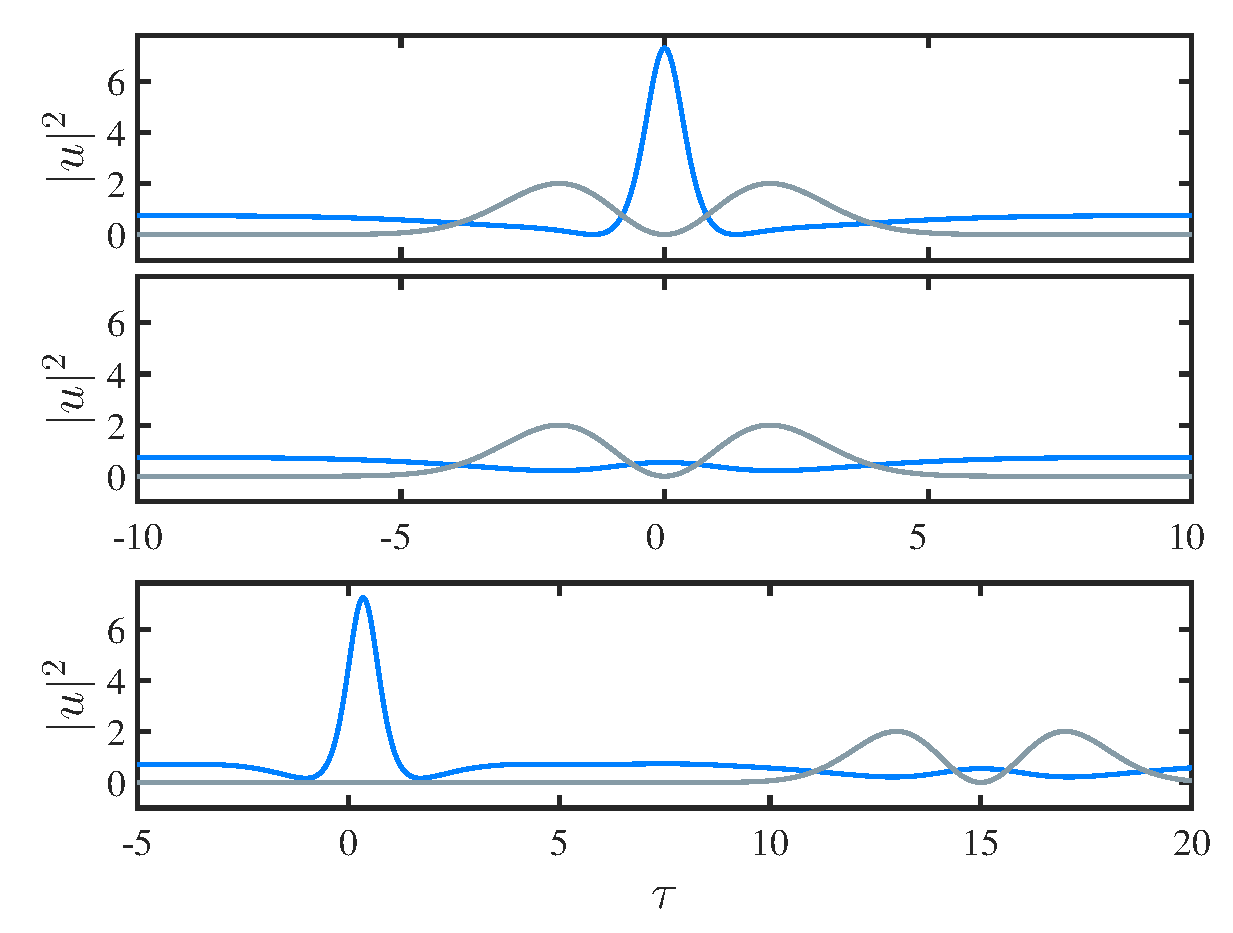
\includegraphics[width=8.5cm]{threeStates.eps}
%  \rule{35em}{0.5pt}
\caption[Temporal Profiles of Fundamental States]{Temporal profiles of the intracavity field envelope $|u|^2$ (blue line) for the most fundamental nonlinear states of the system.  In this example, the effective potential, $V_{\mathrm{eff}} = (\phi')^2$ (solid grey line) is constant in the three panels.  The top panel is an example of a trapped CS (tweezed CS).  The middle panel is an example of no soliton solution (no-CS).  The bottom panel has an effective potential centered at $\tau_0 = 15$.  The CS is located outside of the effective potential, and a no-CS is found inside the effective potential (called non-tweezed CS).  
}
\label{fig:threeStates}
\end{figure}
%%%%%%%%%% Fig  %%%%%%%%%%%%%%%%%%%%%%%%%%%%%%%%%%%%%%

%%%%%%%%%% Fig  %%%%%%%%%%%%%%%%%%%%%%%%%%%%%%%%%%%%%%
\begin{figure}[t!]
\centering
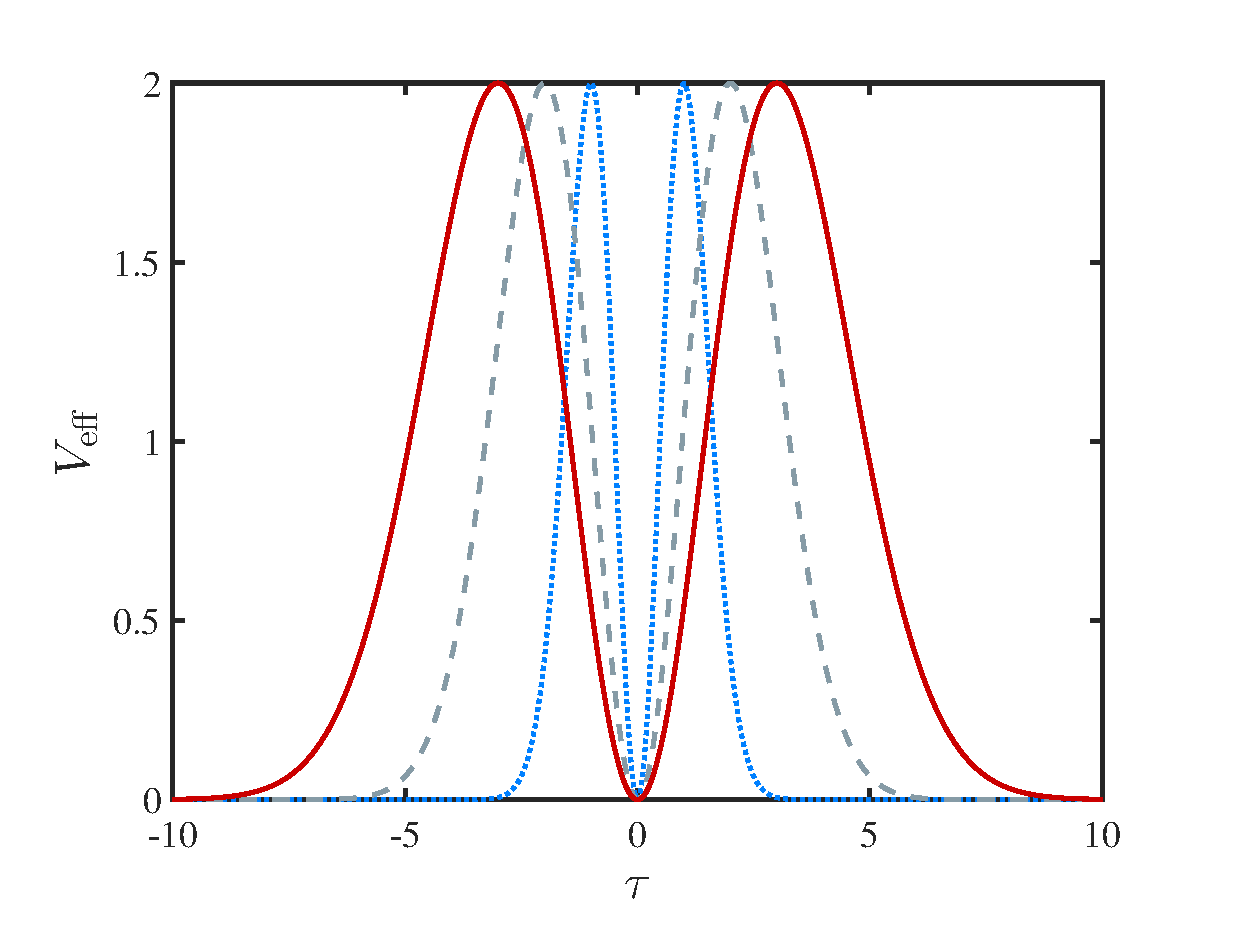
\includegraphics[width=8.5cm]{potentials.eps}\\
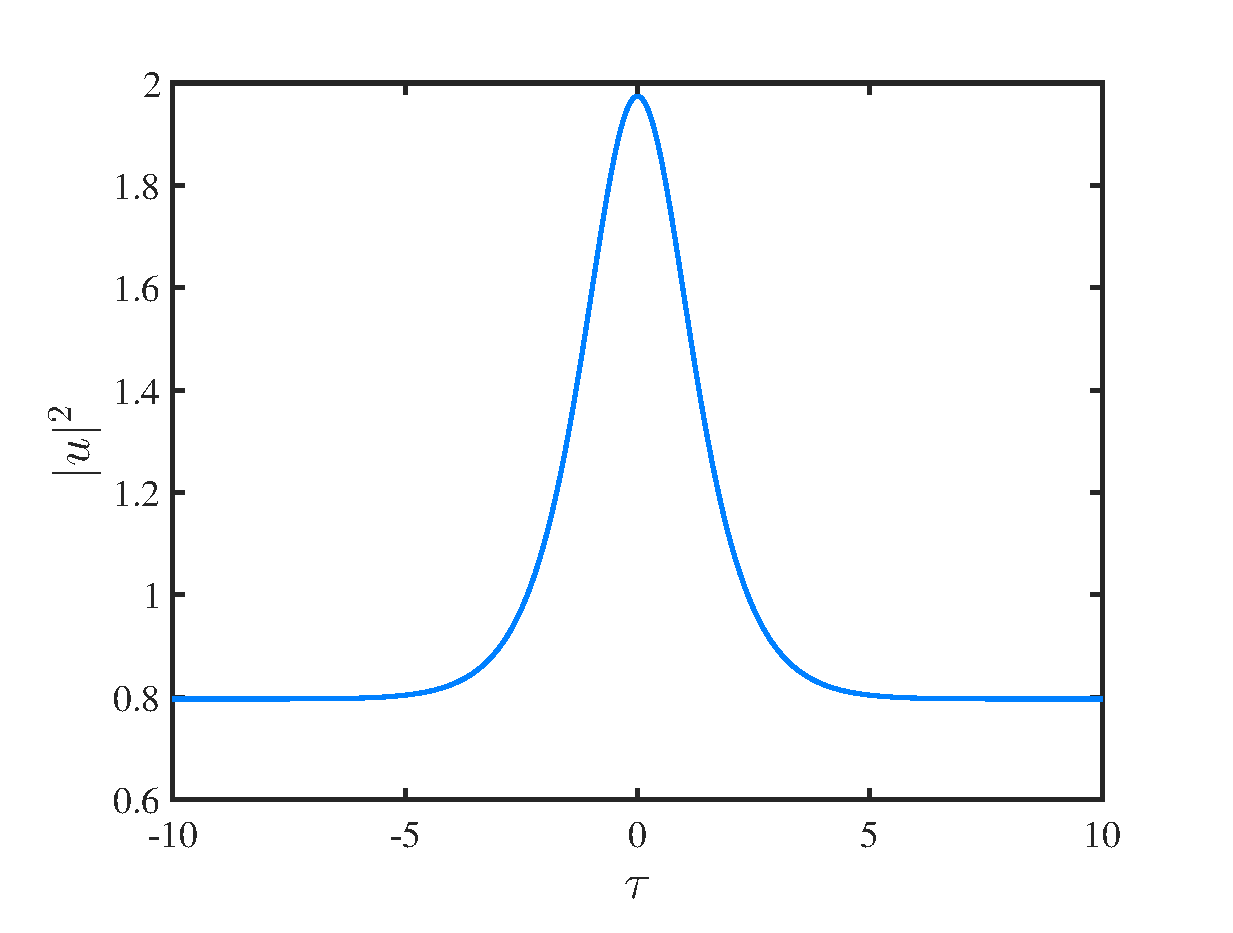
\includegraphics[width=8.5cm]{noTrapCS.eps} 
%  \rule{35em}{0.5pt}
\caption[Tweezers of Narrow, Natural, and Wide Widths]{(a) Tweezers consisting of effective potentials of constant height with narrow, natural and wide widths.  The narrow width tweezer (blue dotted line) is composed of phase modulation with $\sigma_\phi = 1$ and $h_\phi = 2.3316$ solved with Eq.~(\ref{height}).  The natural width tweezer (grey dashed line) is composed of phase modulation with $\sigma_\phi = 2$ and $h_\phi = 4.6633$ solved with Eq.~(\ref{height}).  The wide width tweezer (red solid line) is composed of phase modulation with $\sigma_\phi = 3$ and $h_\phi = 6.9949$ solved with Eq.~(\ref{height}). (b) The density of a cavity soliton in the absence of a tweezer, which has a natural width of ~1.5.  
}
\label{fig:Veff}
\end{figure}
%%%%%%%%%% Fig  %%%%%%%%%%%%%%%%%%%%%%%%%%%%%%%%%%%%%%
We explore the existence and dynamical properties for tweezed cavity soliton (CS) for the effective potential described by $V_{\mathrm{eff}} = (\phi')^2$ (also referred to as the ``tweezer'').   The three qualitatively different scenarios correspond to (a) CS in tweezer, (b) CS outside tweezer, and (c) no-CS are the fundamental nonlinear states of the system, whose profiles for specific phase-modulation parameters $\sigma_\phi = 2$ and $h_\phi=4.6633$ (corresponds to a tweezer of height 2) are displayed in Fig.~\ref{fig:threeStates}.  The top panel depicts a tweezed CS, the middle panel corresponds to no-CS, and the bottom to a non-tweezed CS (a CS outside the tweezer, with no-CS inside the tweezer).  We observe that, for given values of $\sigma_\phi = 2$ and $h_\phi$ for the phase modulation Eq.~(\ref{phi}), there are critical values of $\beta$ and $\tau_f$ in Eq.~(\ref{tau0}) corresponding to thresholds between these fundamental states.  We observe in the NCVA formulation the existence of only two states: a tweezed CS and a no-CS solution.  

We now proceed to provide a characterization of the existence of the three states for the full LL Eq.~(\ref{eq:LLETweeze}) and compare to the results of the NCVA with respect to the parameters $\beta$ and $\tau_f$.  In what follows, we study different tweezing possibilities over the parameter space spanned by $\tau_f$, the final temporal displacement, and $\beta$, the degree of adiabaticity for the speed of the tweezer.  A fully tweezed CS will correspond to a CS that stays inside the effective potential as the tweezer is displaced.  

Rather than analyzing the individual evolution of temporal profiles, we can express the various states by the power contained inside and outside of the effective potential.  For the full LL model, the CS temporal density $\rho = |u|^2$ and the no-CS temporal density $\rho_0 = |u_{\rm{no\text{-}CS}}|^2$ are expressed by the power inside the tweezer $P_{\rm I}(z)$ and outside the tweezer $P_{\rm O}(z)$ which are given respectively by 
\begin{align}
P_{\rm I}(z) = \int_{\rm D} (\rho - \rho_0) d\tau, \label{Pin} \\
P_{\rm O}(z) = \int_{\bar{\rm D}} (\rho - \rho_0) d\tau, \label{Pout}
\end{align} 
where ${\rm D} = [ -\sigma, \sigma]$ is the domain of the tweezer which is defined as a small symmetric interval around $\tau_0$ between the maxima of the effective trap and its complement, $\bar{\rm{D}}$.  We need to subtract the no-CS power, $\rho_0$ in order to counter the effects of the pedestal (constant steady state) and insure the power for a CS is positive.  The total power of the system is given by 
\begin{align}
P_{\rm Tot} = \int  (\rho - \rho_0) d\tau.
\end{align}
Recall that in the construction of the NVCA ansatz we already subtracted out the effects of the background pedestal.  For the NCVA, we use the variational parameters and construct the CS temporal density $\bar{\rho} = |\bar{u}|^2$ and extract the power inside the tweezer $P_{\rm I}(z)$ and outside the tweezer $P_{\rm O}(z)$ which are given, respectively, by 
\begin{align}
P_{\rm I}(z) = \int_{\rm D} \bar{\rho }d\tau, \label{PinNCVA} \\
P_{\rm O}(z) = \int_{\bar{\rm D}} \bar{\rho } d\tau, \label{PoutNCVA}
\end{align} 
where ${\rm D}$ and $\bar{{\rm D}}$ are the same intervals described above.
%Due to the construction of the NCVA ansatz, $\rho_0 = 0$ since the background pedestal is removed and the no-CS solution of the NCVA tends toward zero (not $v$ as described by the full LL model). 
The power ratio parameters inside, $Q_{\rm I}$, and outside, $Q_{\rm O}$, the tweezer are then defined, respectively, by 
\begin{align}
Q_{\rm I} = \frac{P_{\rm I}(0) - P_{\rm I}(z_f)}{P_{\rm Tot} },\label{QIn} \\ 
Q_{\rm O}=  \frac{P_{\rm O}(0) - P_{\rm O}(z_f)}{P_{\rm Tot} }.
\label{QOut}
\end{align}
By considering $Q_{\rm I}$ and $Q_{\rm O}$, we can effectively find the thresholds between the various states in the relevant ($\beta$, $\tau_f$) parameter space.  


For example, if we begin with a steady state CS inside the tweezer at $\tau_0=0$ and move with a given $\beta$ and $\tau_f$, then a perfectly tweezed CS will result on the same powers at $z=0$ as $z = z_f$ such that $P_{\rm I}(0) =  P_{\rm I}(z_f)$ as well as $P_{\rm O}(0) = P_{\rm O}(z_f)$, making the power ratios $Q_{\rm I} = Q_{\rm O} = 0$.   If the CS dissipates perfectly and we are left solely with no-CS inside the tweezer, then $Q_{\rm I} = 1$ and  $Q_{\rm O} = 0$.  For the final non-tweezed CS state, at $z=z_f$ the CS is completely outside the tweezer, and a no-CS is inside the tweezer, at which point $Q_{\rm I} = Q_{\rm O} = 1$ .   

For our analysis, we select three tweezers with a fixed height and a narrow, natural, and wide width corresponding to $\sigma_\phi = 1$, 2, and 3, respectively.  In order to maintain a constant maximum height of the effective potential $V_{\rm eff}$ equal to 2 (such that we have a deep enough trap to contain the CS and is the height of a natural CS in the absence of a tweezer [see Fig.~\ref{fig:Veff}(b)]), we solve for the height of Eq.~(\ref{phi}) 
\begin{align}
h_\phi = \frac{\sqrt{2} \sigma_{\phi}^2}{\max [\tau \exp(-\tau^2/2\sigma_{\phi}^2)]}.
\label{height}
\end{align}
Figure~\ref{fig:Veff}(a) depicts the effective potentials $V_{\rm eff} = (\phi')^2$ used in the three tweezer cases we are interested in studying: tweezers with natural width $\sigma_\phi = 2$ (grey dashed line) in Sec.~\ref{section:Regular}.  For extra examples, Appendix~\ref{AppendixC} contains two more examples of tweezers with (i) narrow width $\sigma_\phi = 1$ (blue dotted line) in Sec.~\ref{section:Skinny}, and (ii) wide width $\sigma_\phi = 3$ (red solid line) in Sec.~\ref{section:Fat}.  For comparison, Fig.~\ref{fig:Veff}(b) shows the density of a CS in the absence of a tweezer, which has a natural width $\sigma \approx 1.5$.  For all example cases to follow, we keep the holding beam constant at $u_{\rm in} = 2$.


\subsection{Tweezer with Natural Width}
 \label{section:Regular}
 
 %%%%%%%%%% Fig  %%%%%%%%%%%%%%%%%%%%%%%%%%%%%%%%%%%%%%
\begin{figure}[htb!]
\centering 
\hskip 0.4em 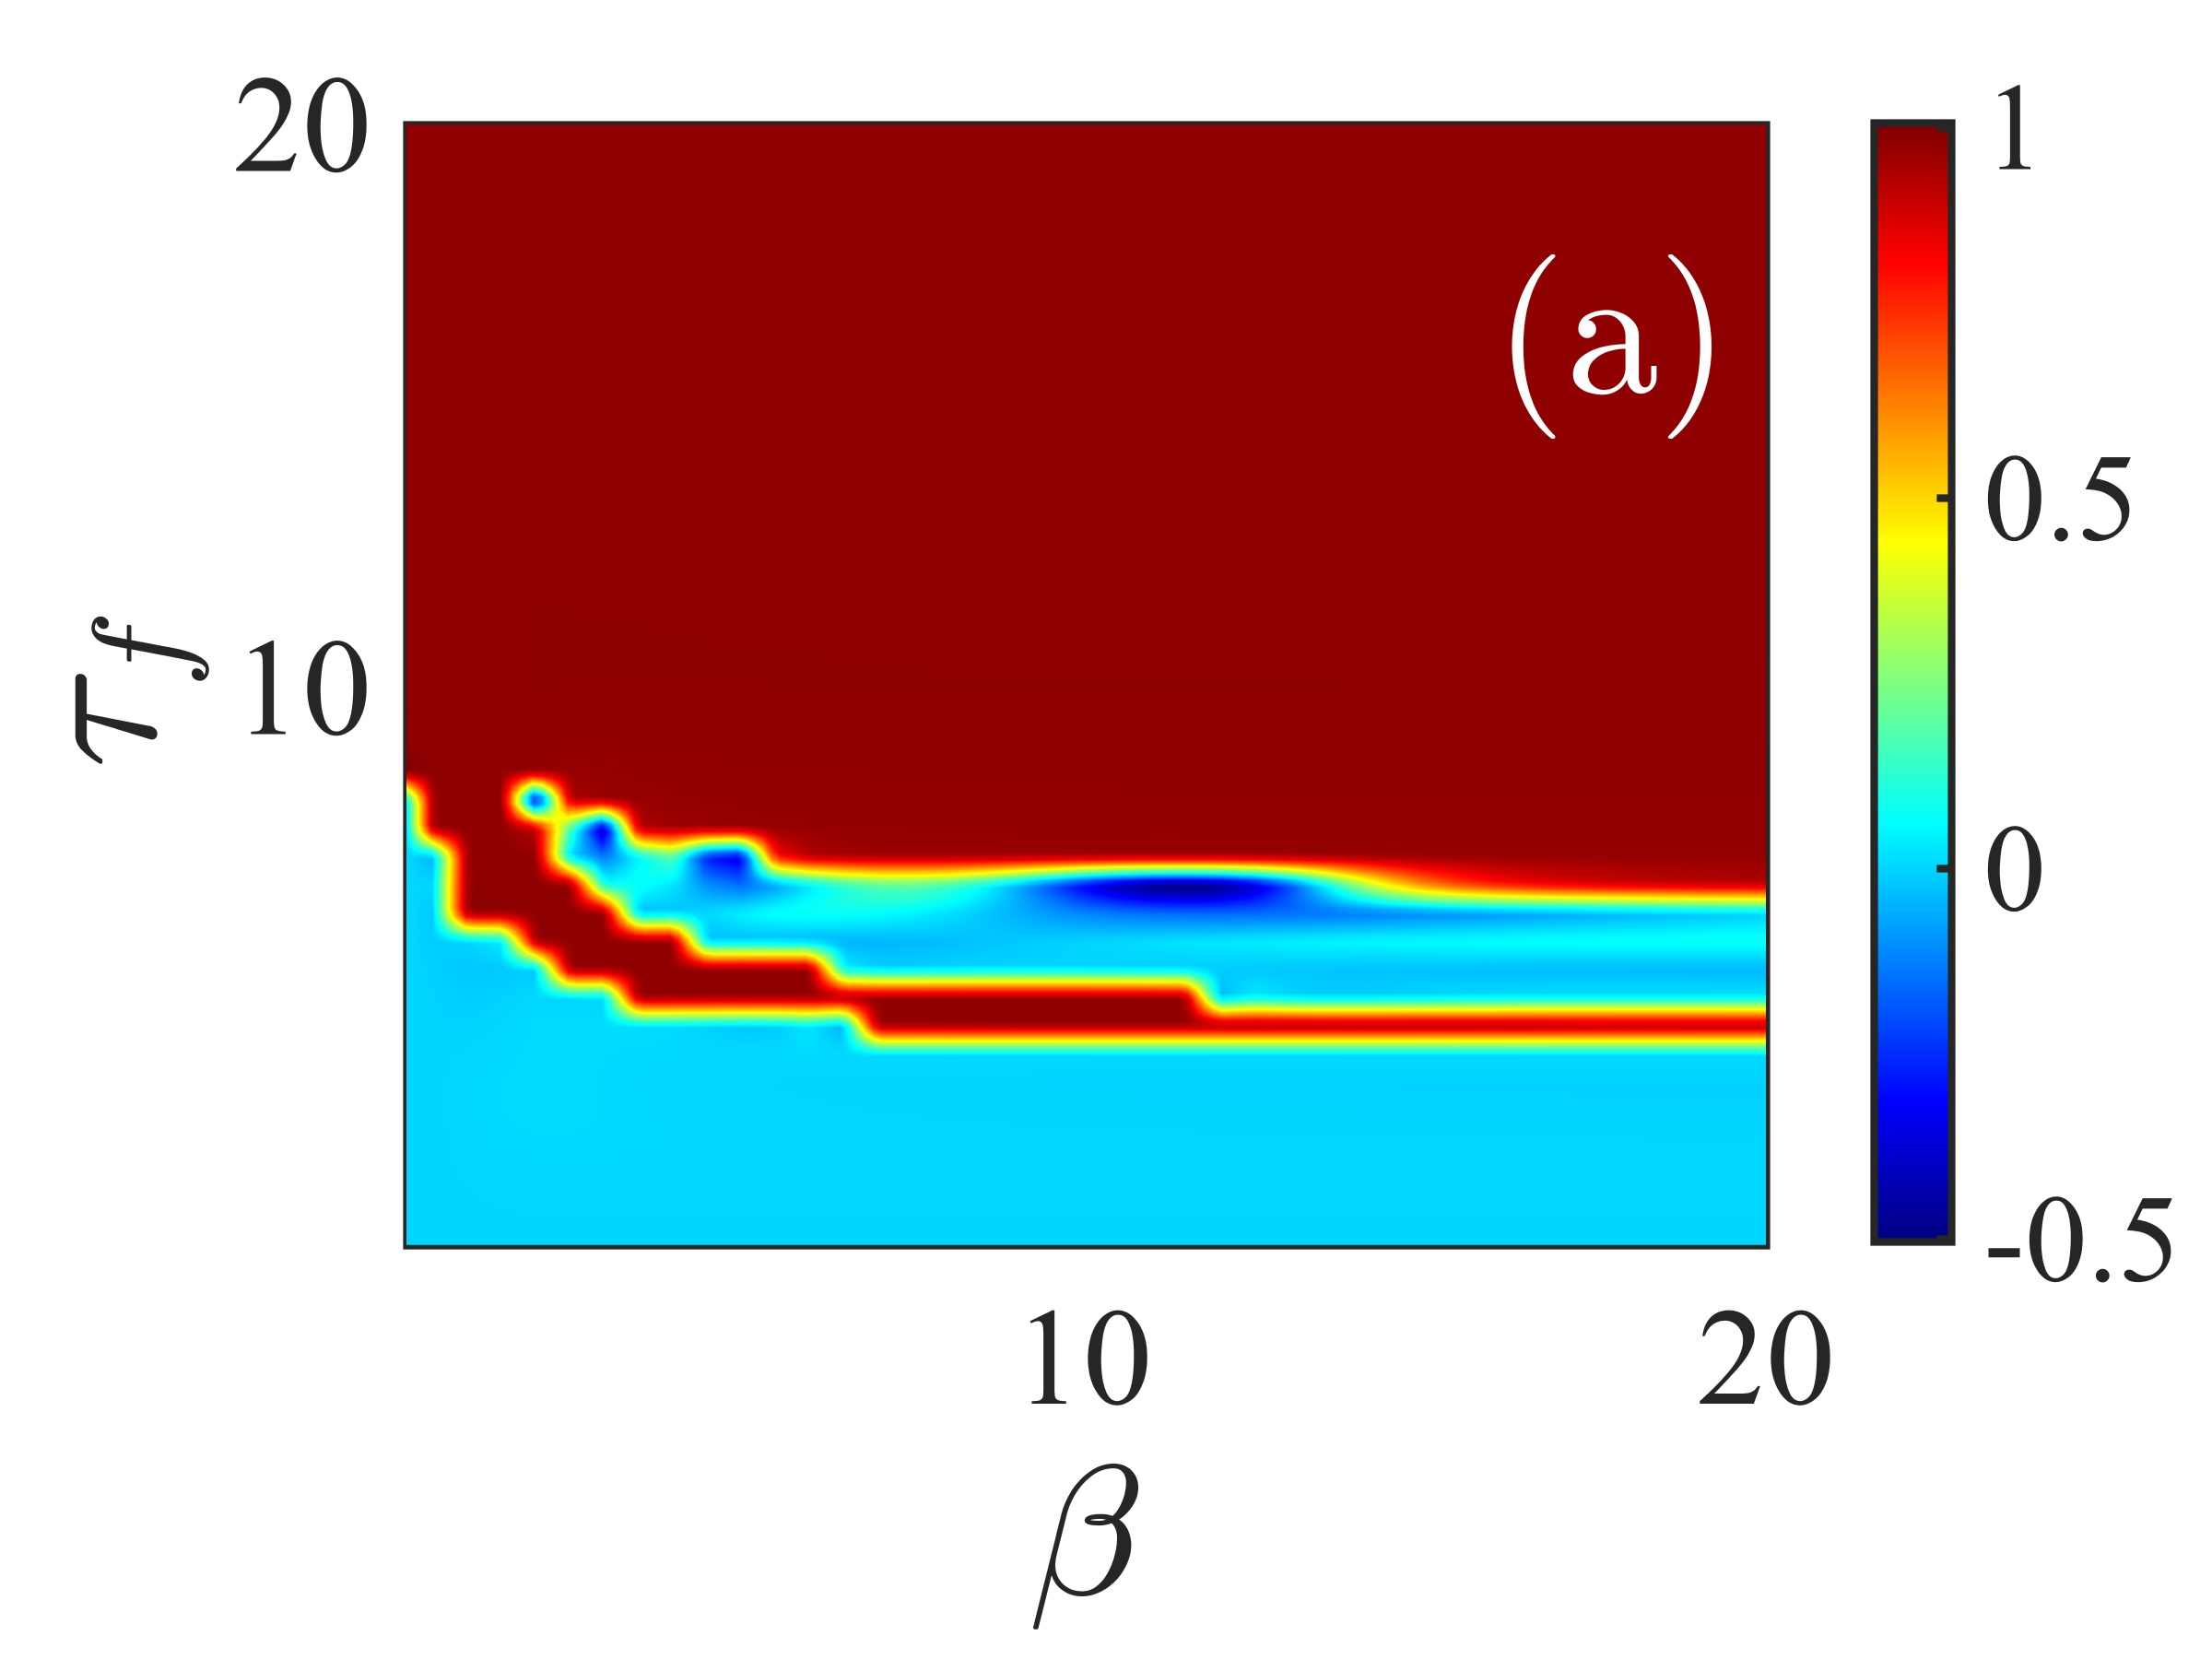
\includegraphics[width=4.2cm]{RegularQIn.jpg}
\hskip -0.5em 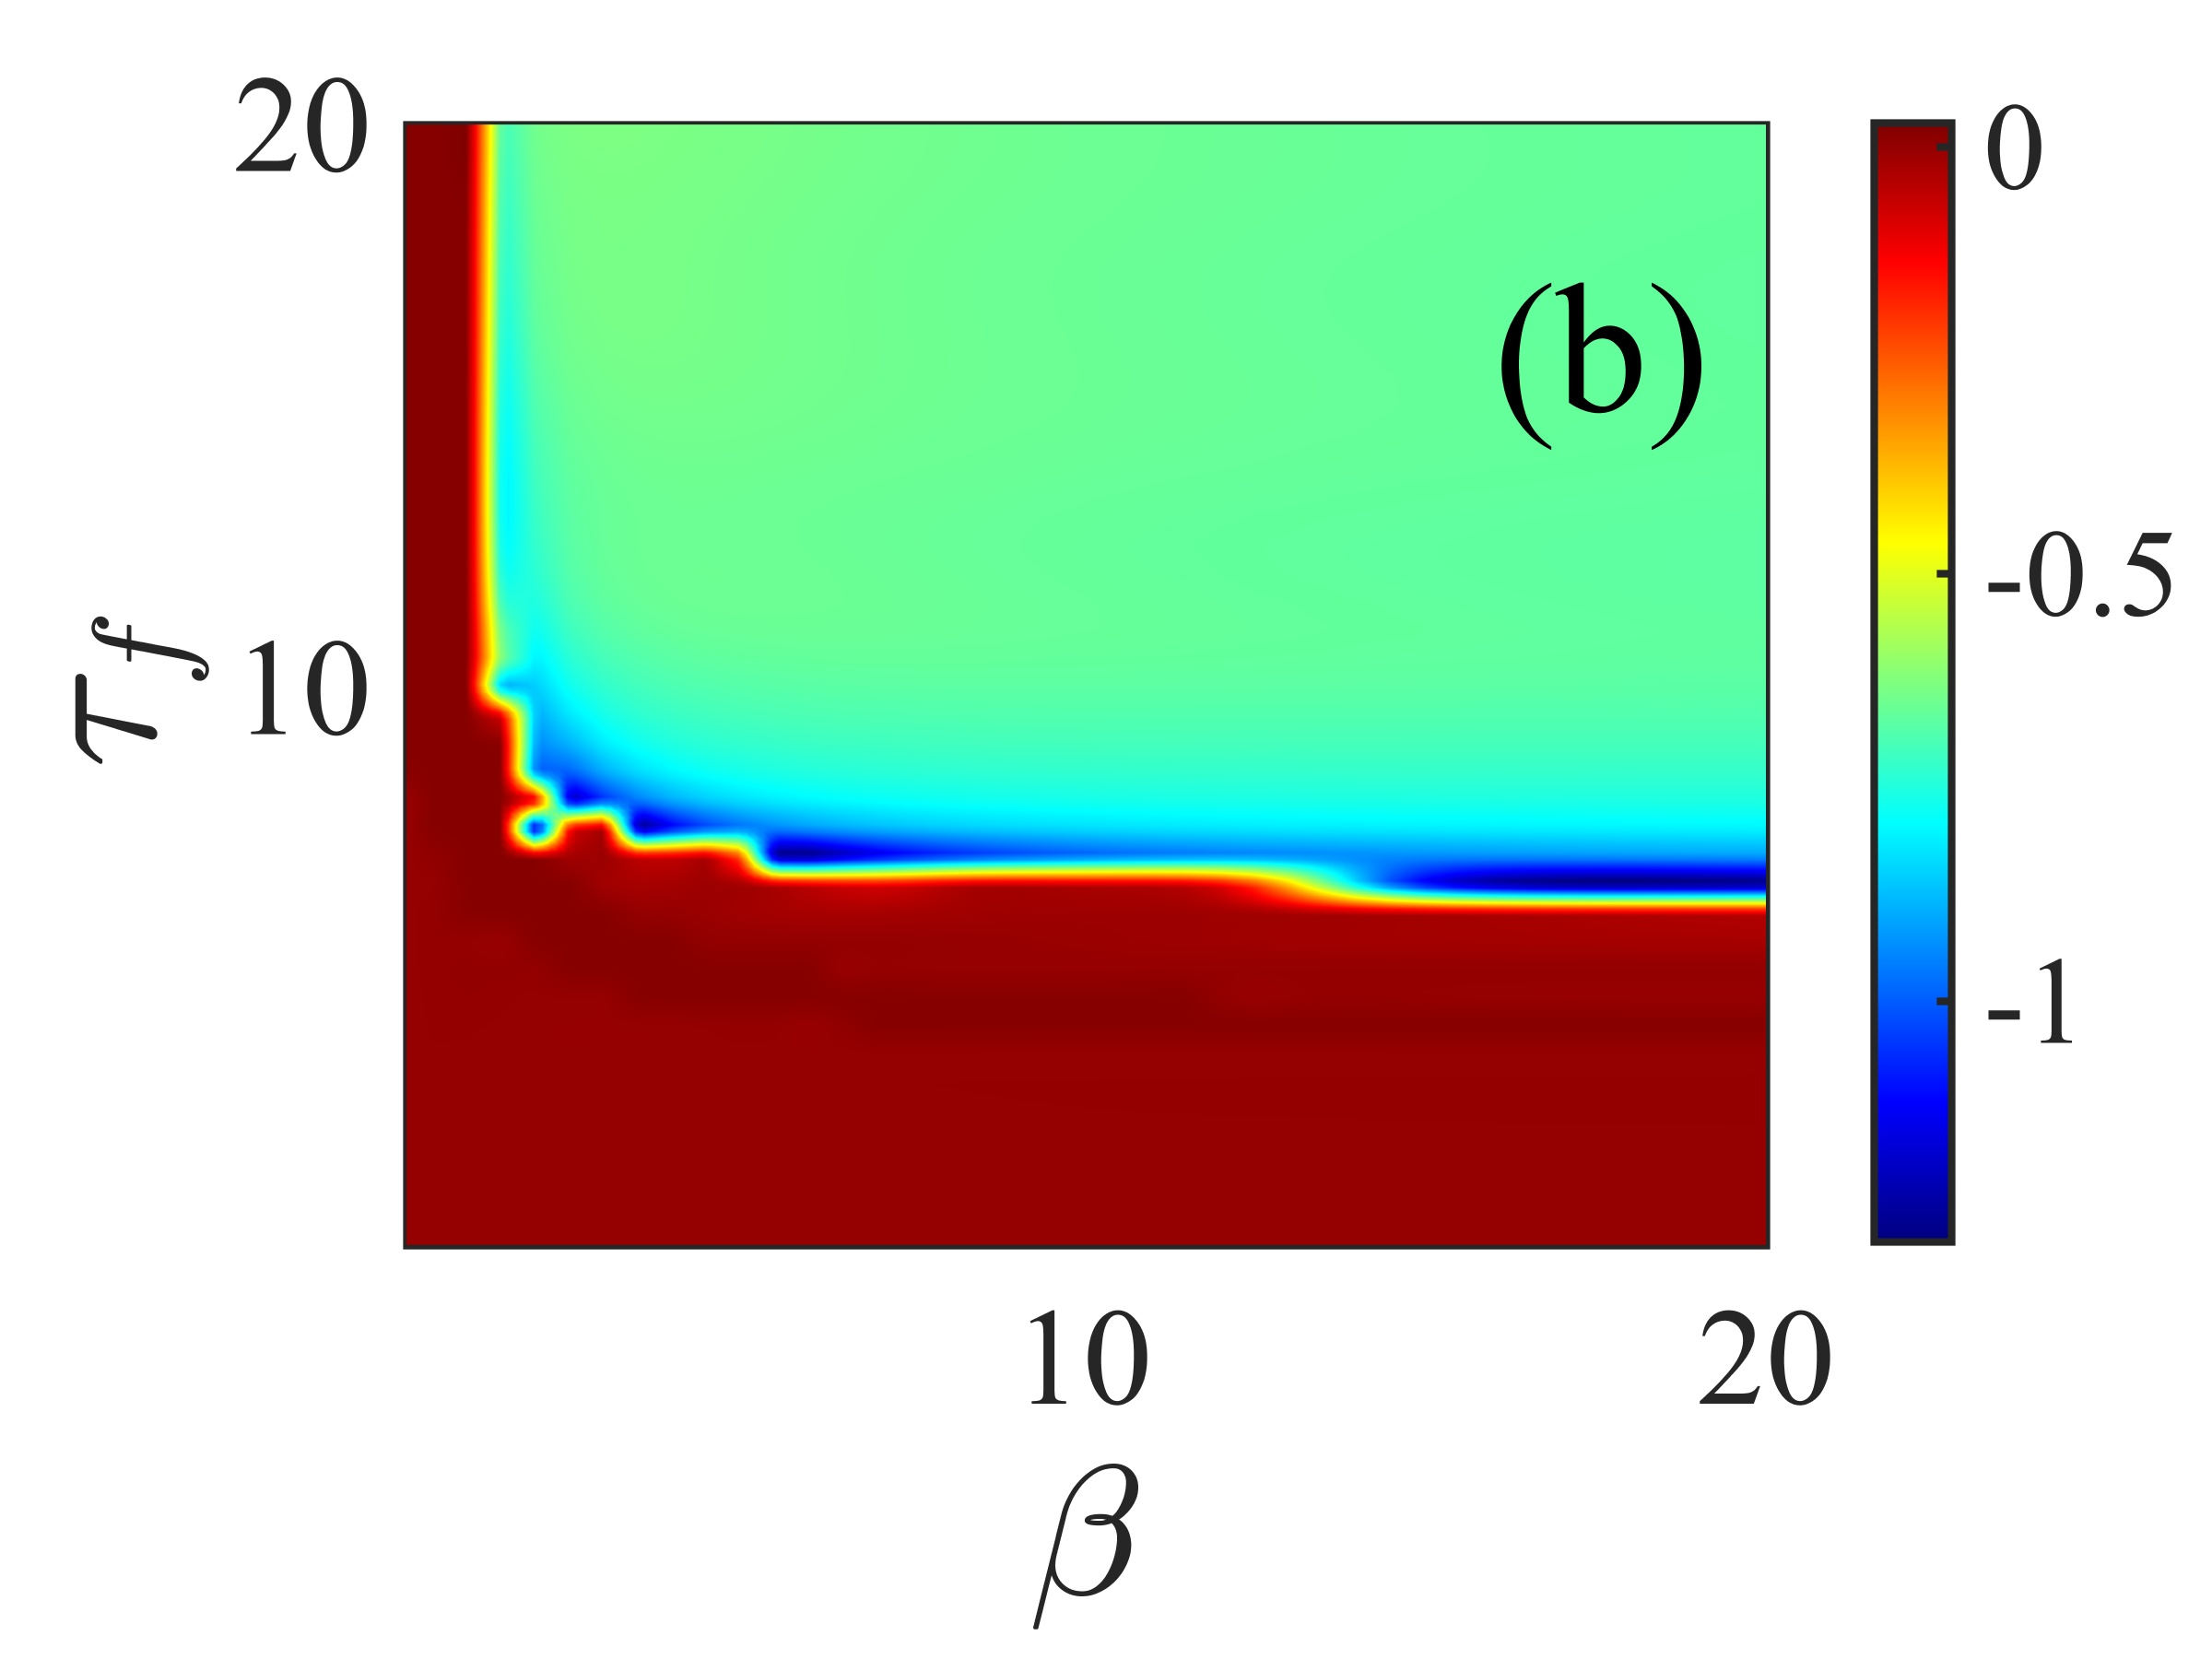
\includegraphics[width=4.2cm]{RegularQOut.jpg} 
\\
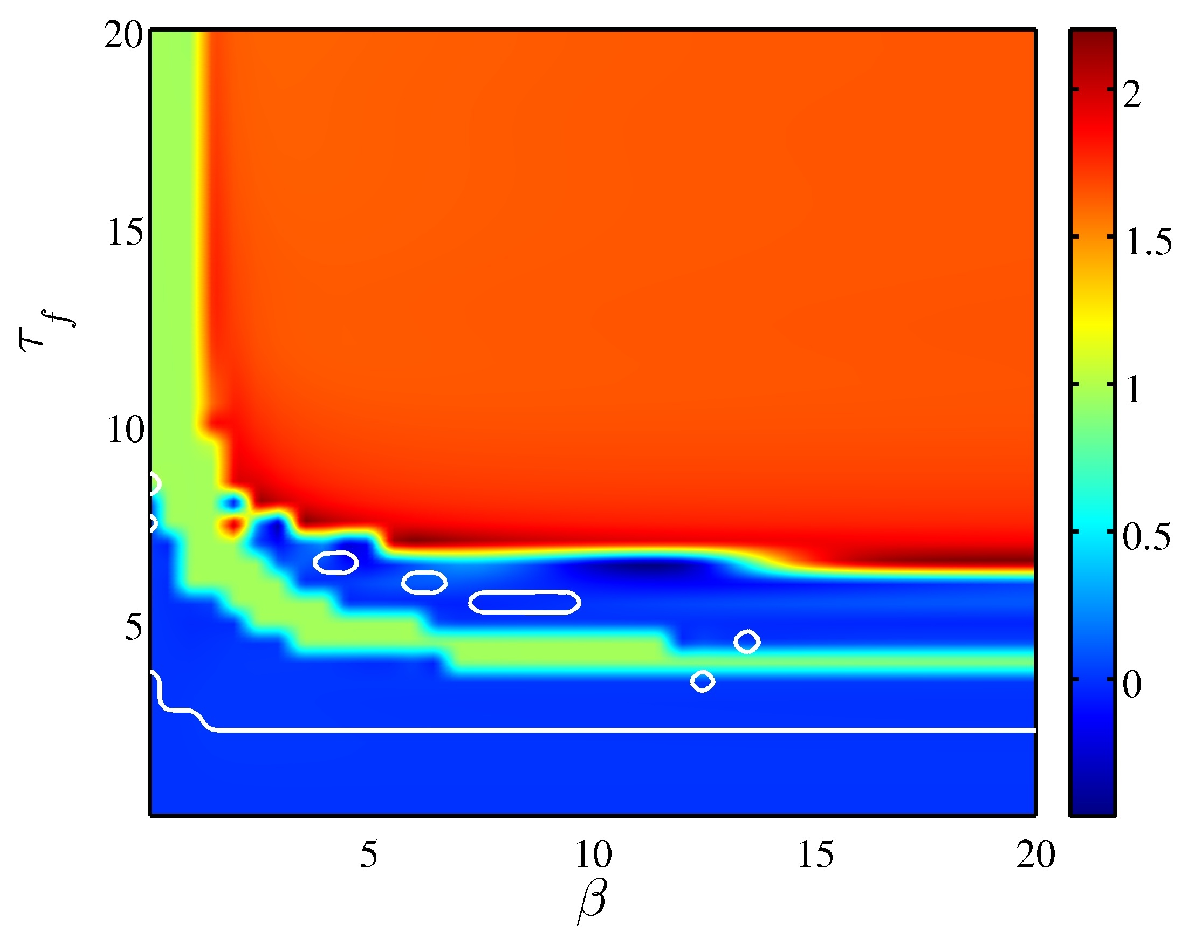
\includegraphics[width=8.5cm]{RegularPDEvODE_rcg_t.eps} 
\vspace{-0.5em}
\caption[Power Ratios Inside and Outside Tweezer with Natural Width]{The density of the power ratios (a) inside and (b) outside of a narrow tweezer width $\sigma_\phi = 2$ and height $h_\phi = 4.6633$.  The detuning for the system is $\Delta =  2.8357$ and each combination of parameter is evolved for $z_f = 10 = 4z^*$, with $z^* = 2.5$.  (a) The power ratio density inside the tweezer $Q_{\rm I}$, where blue ($Q_{\rm I}=0$) is complete power inside the tweezer at $z_f$ and red ($Q_{\rm I}=1$) is no power inside the tweezer at $z_f$.  (b) The power ratio density outside the tweezer $Q_{\rm O}$, where $Q_{\rm O}$ = 0 depicts no change in power.  (c) 
The density of the difference of power ratios inside of a narrow tweezer, $Q_{\rm I} - Q_{\rm O}$ for the full LL model with a single contour at 0.5 (white line) for the NCVA threshold between tweezed and non-tweezed states.  For the difference of power ratios, a value of 1 is a non-tweezed CS, a value of 0.5 is a no-CS, and a value of 0 is a tweezed-CS.  The white contour line distinguishes the NCVA region between a solutions with tweezed CS and dissipative solutions with no-CS.  The LL model has clear regions of state, namely, a tweezed CS in blue region (under the green region), no-CS in the green region, and a non-tweezed CS in orange region.
}
\label{fig:RegularQ}
\end{figure}
%%%%%%%%%% Fig  %%%%%%%%%%%%%%%%%%%%%%%%%%%%%%%%%%%%%%

%%%%%%%%%% Fig  %%%%%%%%%%%%%%%%%%%%%%%%%%%%%%%%%%%%%%
\begin{figure}[htb!]
\centering
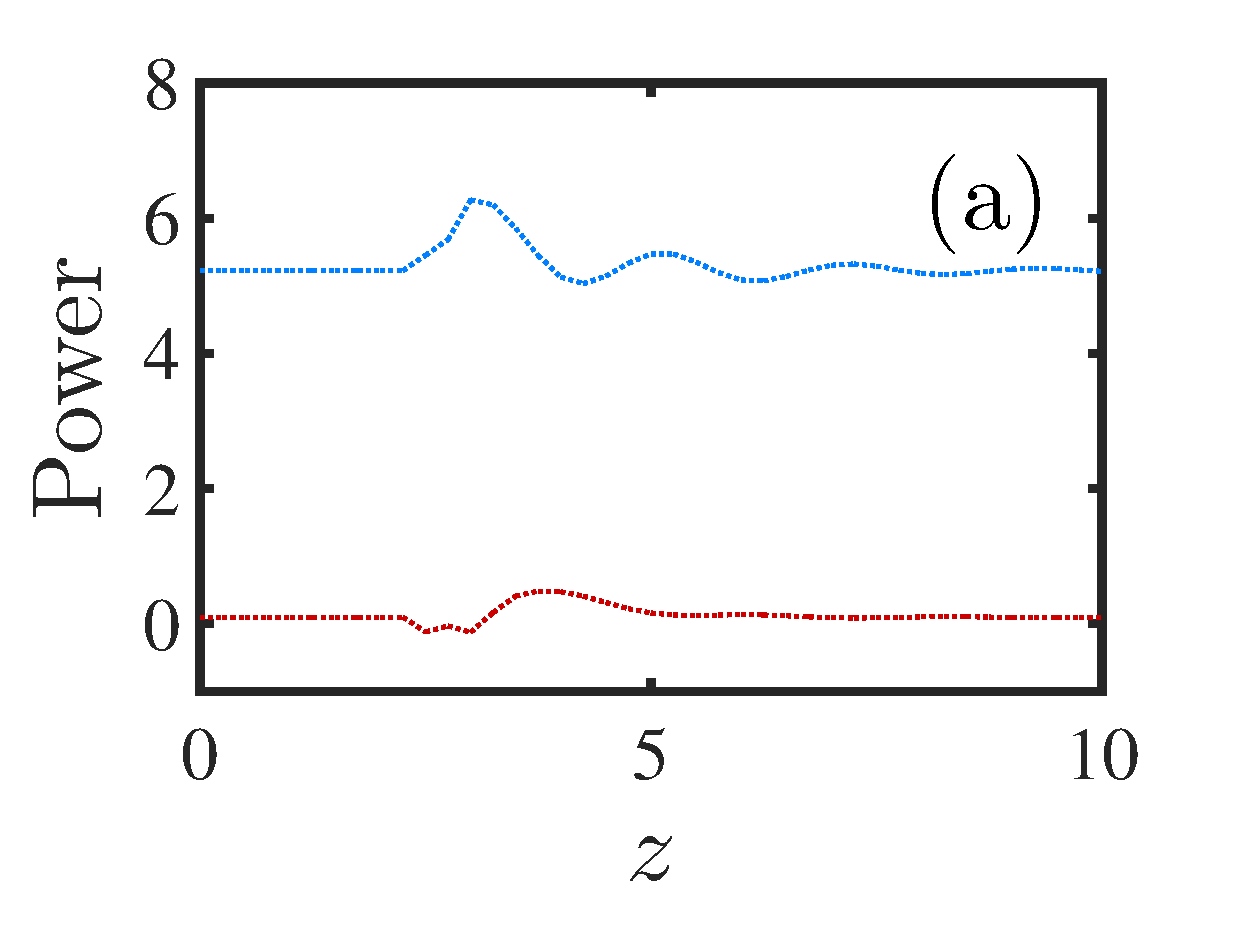
\includegraphics[width=4.2cm]{regularTimeMass1.eps} 
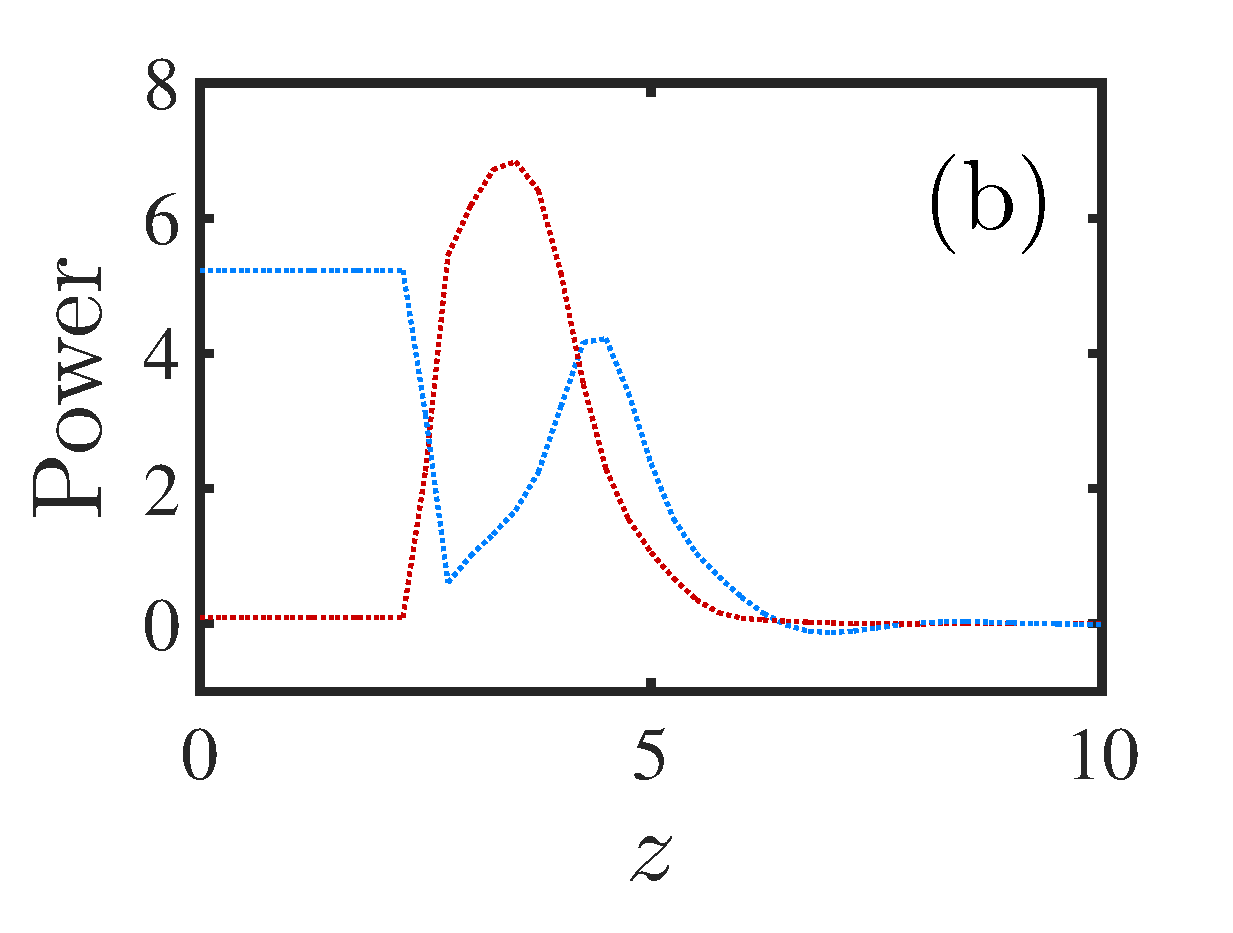
\includegraphics[width=4.2cm]{regularTimeMass5.eps} 
\\
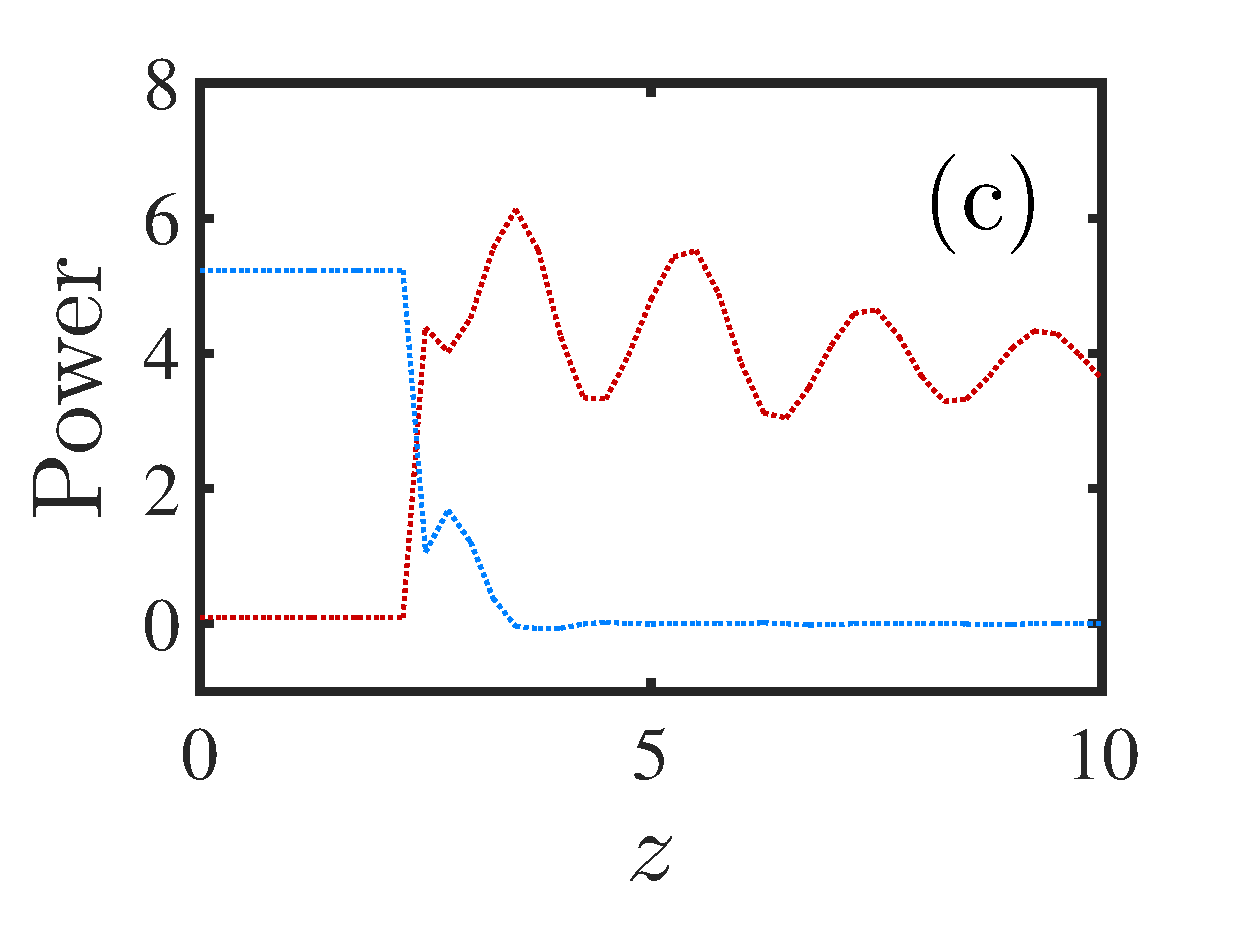
\includegraphics[width=4.2cm]{regularTimeMass3.eps} 
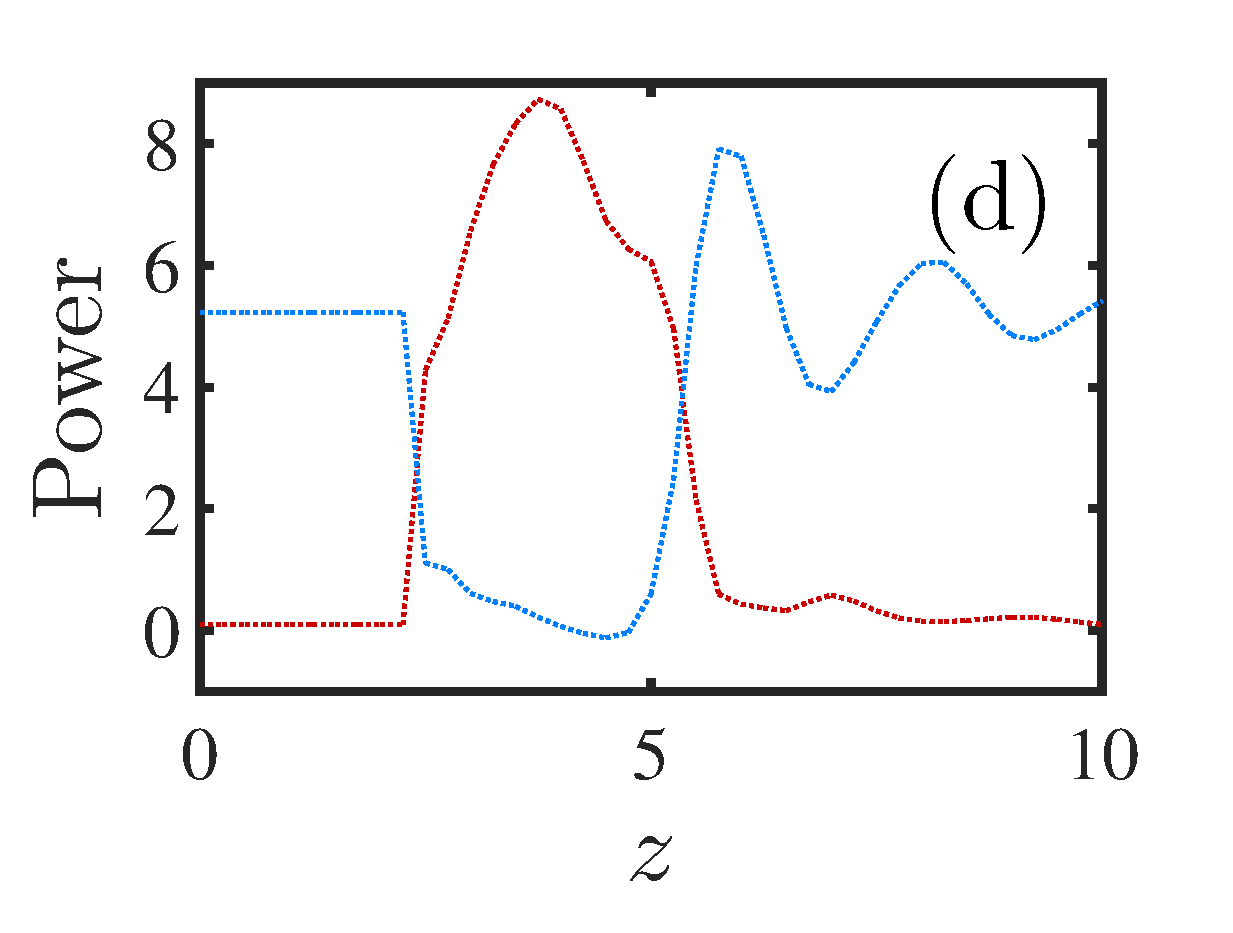
\includegraphics[width=4.2cm]{regularTimeMass6.eps}
\vspace{-0.5em}
\caption[Tweezer with Natural Width Power Comparison]{Comparison of the powers found inside the tweezer $P_{\rm I}$ (red line) and outside the tweezer $P_{\rm O}$ (blue line) for the parameters (a) $\tau_f = 2$ and $\beta=10$, (b) $\tau_f = 4.5$ and $\beta=10$, (c) $\tau_f = 12$ and $\beta=10$ and (d) $\tau_f = 5.5$ and $\beta=8$.  The left top panel (a) has no change in power inside or outside the tweezer which describes a tweezed CS, while right top panel (b) shows power change for no-CS.  The left bottom panel (c) is an example of the tweezer moving too quickly and leaving the CS outside the tweezer (non-tweezed).  The right bottom panel (d) is ``artificial'' tweezing, in which the trap initially loses the CS but but $z_f$ the CS catches up the tweezer.
}
\label{fig:RegularComp}
\end{figure}
%%%%%%%%%% Fig  %%%%%%%%%%%%%%%%%%%%%%%%%%%%%%%%%%%%%%

%%%%%%%%%% Fig  %%%%%%%%%%%%%%%%%%%%%%%%%%%%%%%%%%%%%%
%\begin{figure}[htb!]
%\centering
%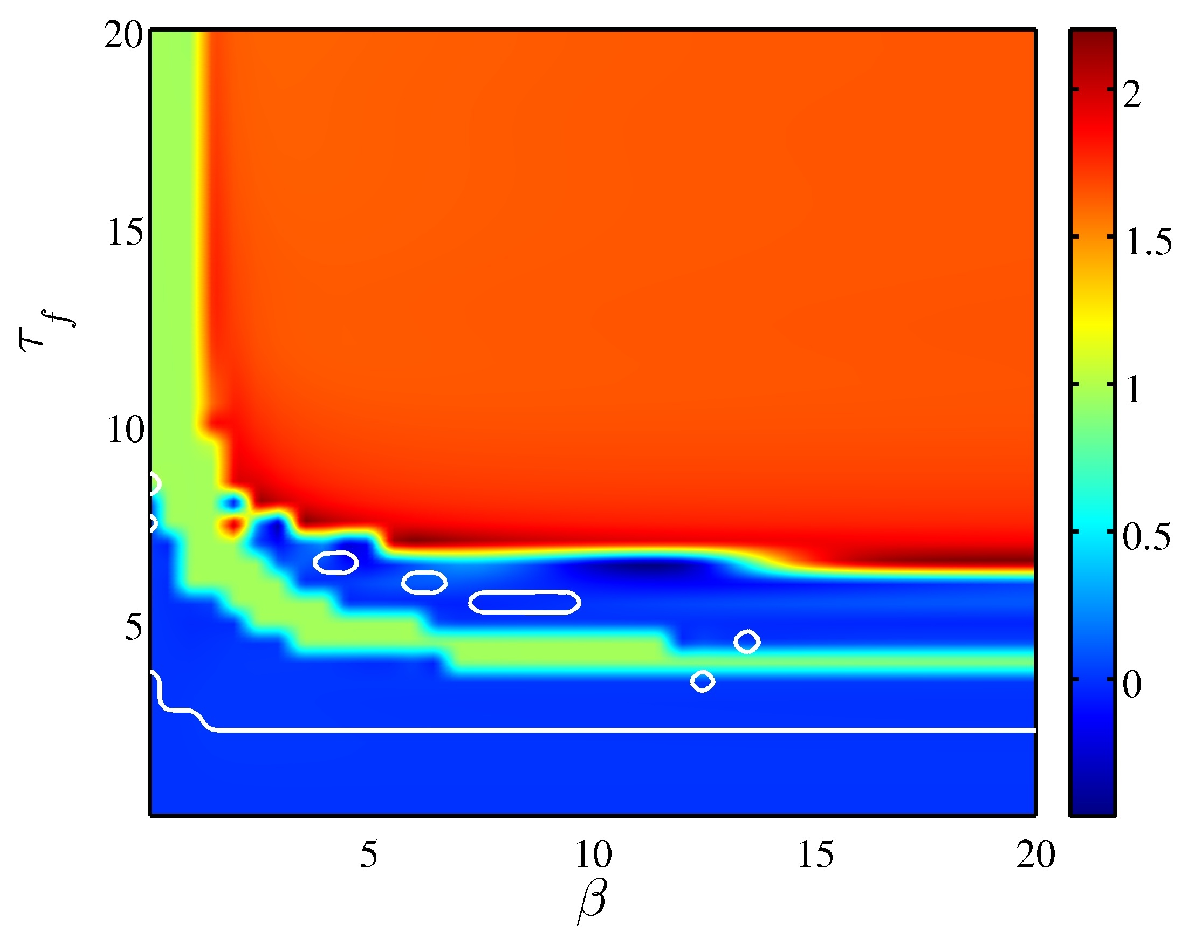
\includegraphics[width=8.5cm]{RegularPDEvODE_rcg_t.eps}
%\caption[Comparison of Power Ratios of Natural Tweezer for LL Model and NCVA]{Comparison of difference in power ratios between the NCVA and LL model as in Fig.~\ref{fig:SkinnyVsNCVA} but for a natural tweezer.  Same layout as Fig.~\ref{fig:SkinnyVsNCVA}.  The NCVA distinguishes a threshold between tweezed and no-CS soltions at $\approx 2.5$ and regions of tweezed CS for larger parameters.  The LL model has clear regions of state, namely, a tweezed CS in blue region (under the green region), no-CS in the green region, and a non-tweezed CS in orange region.
%}
%\label{fig:RegularVsNCVA}
%\end{figure}
%%%%%%%%%% Fig  %%%%%%%%%%%%%%%%%%%%%%%%%%%%%%%%%%%%%%

In this case study, we are interested in a tweezer with a natural width $\sigma_\phi = 2$ and height $h_\phi = 4.6633$ by Eq.~(\ref{height}). 
%
For the full LL Eq.~(\ref{eq:LLETweeze}), the steady state CS is found centered at $\tau_0 = 0$ using a Newton-Krylov solver and the power-balance constraint Eq.~(\ref{LLConstraint}) which selects a detuning parameter value of $\Delta =  2.8357$.
%
The same $\Delta$, $\sigma_\phi$, and $h_\phi$ are used in the NCVA with a Newton-Krylov solver to find the initial variational parameters for the system.  
%
The parameter space for $\beta$ and $\tau_f$ are discretized into 41 steps between 0.1 and 20, giving 1681 combinations for $\tau_0(z)$ [Eq.~(\ref{tau0})].  
%
The full LL Eq.~(\ref{eq:LLETweeze}) is solved using a Runge-Kutta method in time and finite differences in space and the NCVA system of ODEs are solved using Matlab's ode15s.  It is important to note, the NCVA requires a stiff ODE solver to produce the numeric results. 
%
Both the full LL equation and NCVA evolve until $z_f = 10 = 4z^*$, with $z^* = 2.5$ which ensures that the tweezed and/or non-tweezed CS have enough time to converge towards their steady state. 

As described in the previous section, we calculate $Q_{\rm I}$ from Eq.~(\ref{QIn}) and $Q_{\rm O}$ from Eq.~(\ref{QOut}) for all parameter combinations.  Figure~\ref{fig:RegularQ} depicts the density of these power ratios inside (Fig.~\ref{fig:RegularQ}(a)) and outside (Fig.~\ref{fig:RegularQ}(b)) the natural tweezer.  In order to identify the different dynamical regions, both $Q_{\rm I}$ and $Q_{\rm O}$ need to be analyzed simultaneously.  For example $Q_{\rm I}$ = 0 is either a no-CS for $Q_{\rm O}=0$ or a non-tweezed CS for $Q_{\rm O}=1$.  For easier interpretation of the results, we use the difference in power ratios, $Q_{\rm diff} = Q_{\rm I} - Q_{\rm O}$, such that the values $Q_{\rm diff} = 0, 0.5$, and 1, respectively, represent tweezed-CS, no-CS, and non-tweezed CS.  The $Q_{\rm diff}$ in Fig.~\ref{fig:RegularQ}(c) clearly defines three fundamental states: a tweezed CS for all $\beta$ when $\tau_f < 4$ (blue region), no-CS (green region), and a non-tweezed CS (orange/red regions).  Please note that the blue inlet region between the green and orange regions in Fig.~\ref{fig:RegularQ}(c) is ``artificial'' tweezing (an example is given in Sec.~\ref{section:Fat}).  In this region, the tweezer initially drags the CS but the CS is eventually left behind by the trap; however, the CS remains in motion and catches up to the trap by $z = z_f$, and the CS reenters the trap at $\tau_f$ which is measured in our power quotient.  The threshold for the existence of the tweezed CS with a natural tweezer is larger than we found for a narrow tweezer and occurs at $\tau_f \approx 4$.  The NCVA solutions only have two fundamental states: (i) a tweezed CS or (ii) a no-CS solution (there is no NCVA solution in which the tweezer leaves behind a CS).  Therefore, it is not necessary to use $Q_{\rm O}$ since both states result in $Q_{\rm O} \approx 0$.  Figure~\ref{fig:RegularQ}(c) depicts a single contour (white line) of the $Q_{\rm diff} = 0.5$ superimposed on the density of $Q_{\rm diff}$ of the full LL model.  This figure allows for a direct comparison of the threshold between a tweezed CS and no-CS solution of the NCVA (white line) and the state regions of the full LL model.  The NCVA also has islands of tweezed CS for larger values of $\tau_f$ and $\beta$ which do not exist in the full LL model.

%%%%%%%%%% Fig  %%%%%%%%%%%%%%%%%%%%%%%%%%%%%%%%%%%%%%
\begin{figure}[t!]
\centering
\hskip 0.4em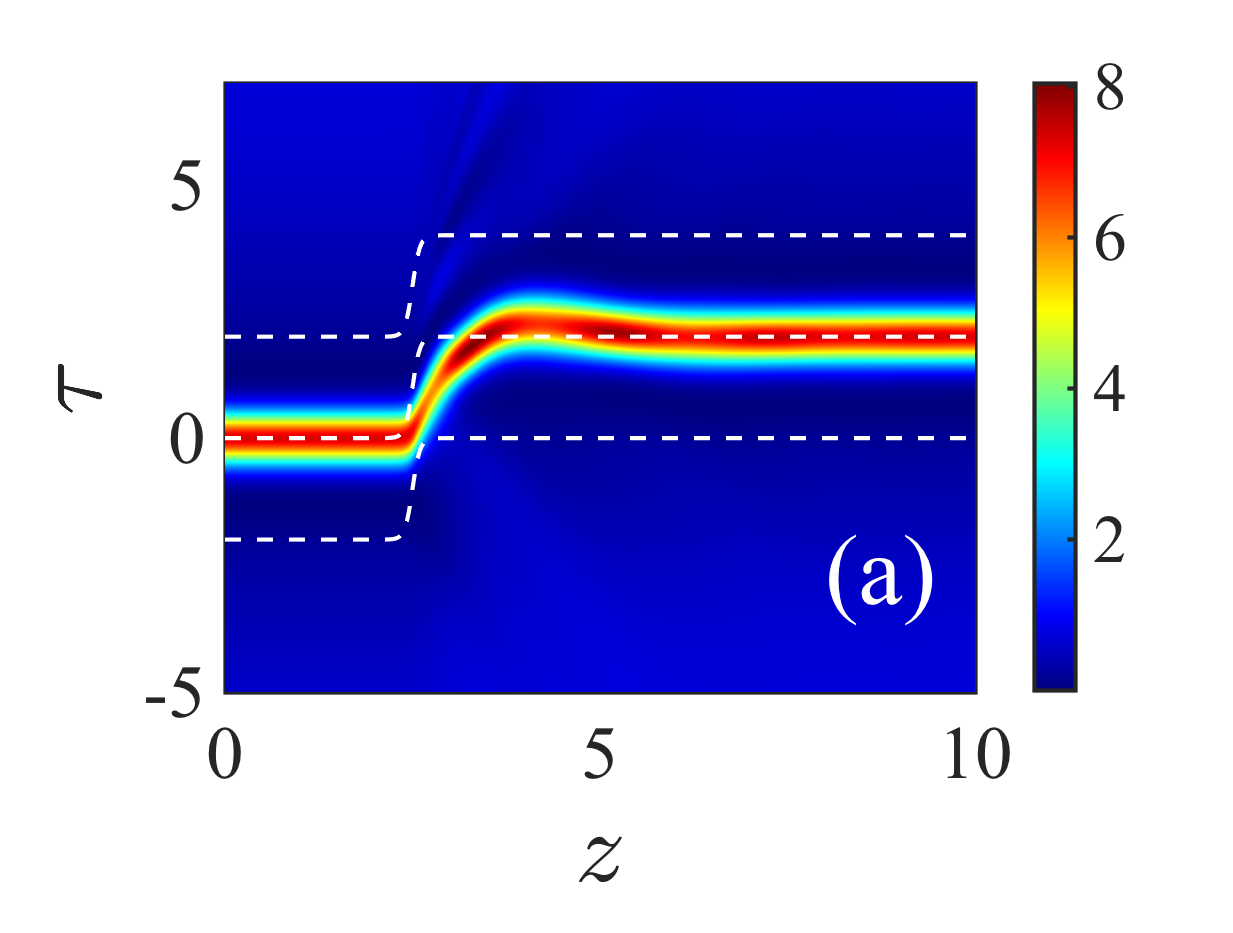
\includegraphics[width=4.2cm]{regularDensity1.eps} 
\hskip -0.5em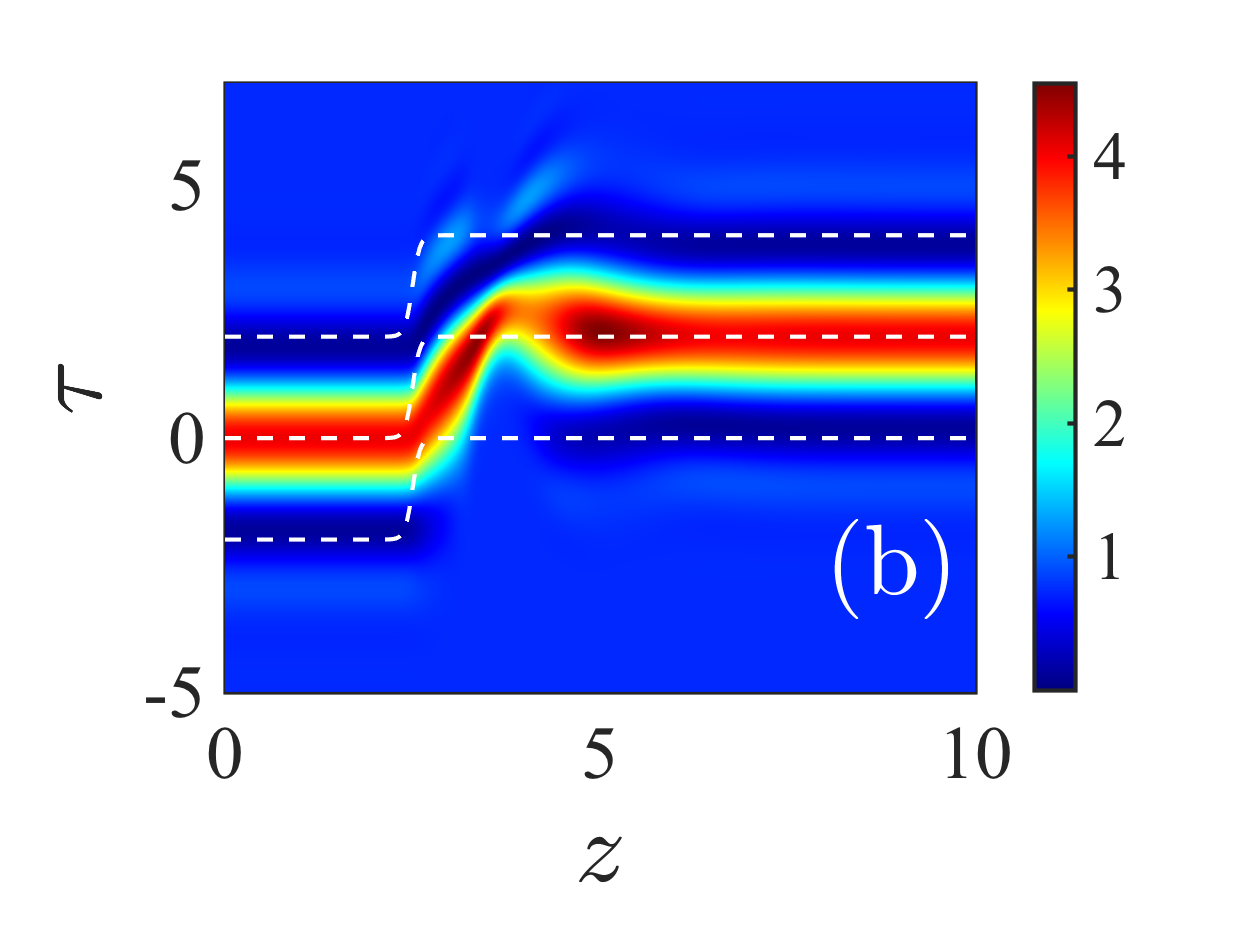
\includegraphics[width=4.2cm]{regularNCVADensity1.eps} 
\\
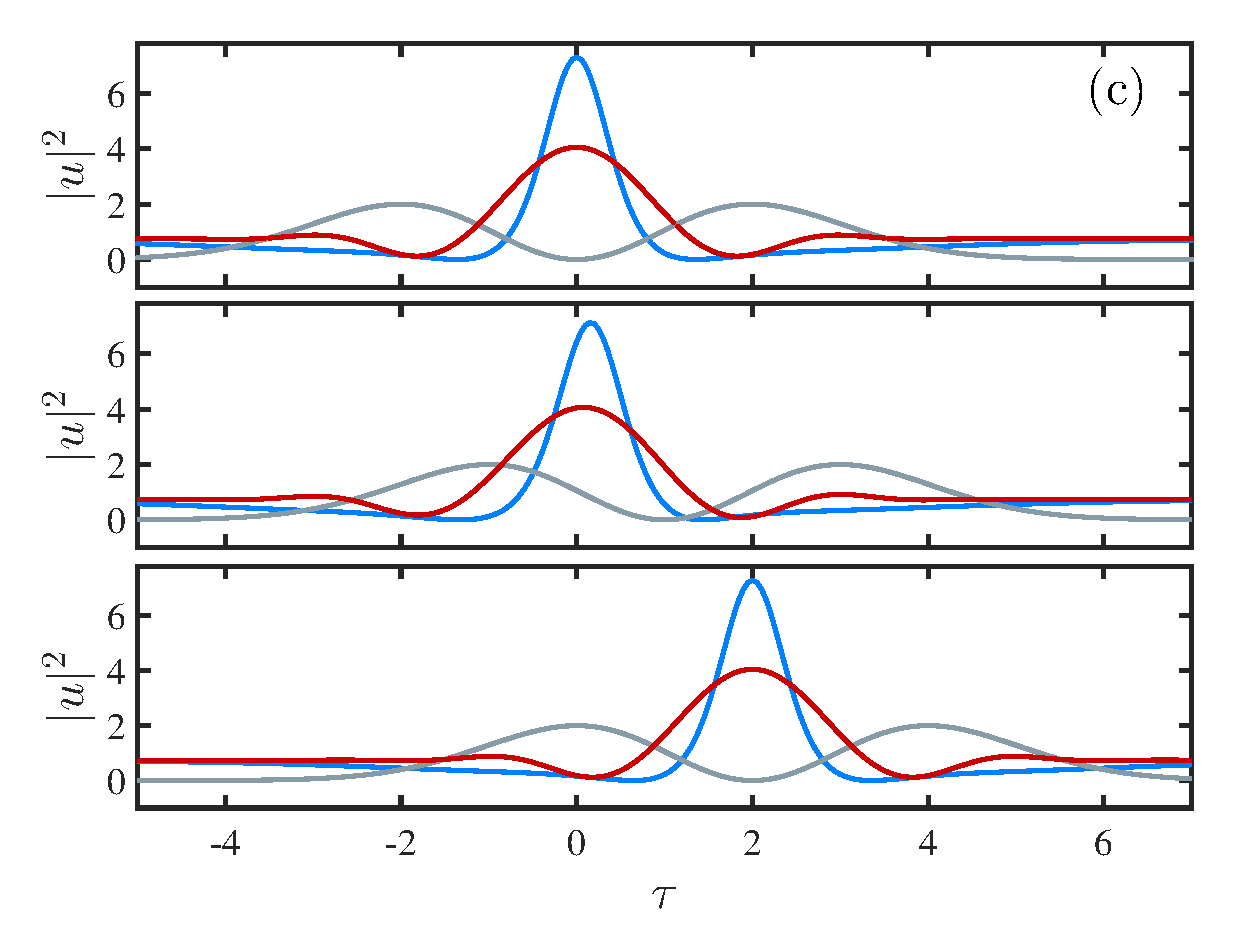
\includegraphics[width=8cm]{regularTimeSeries1.eps} 
\vspace{-0.5em}
\caption[Dynamic Evolution of Natural Tweezer with Tweezed CS]{Example of the density evolution for the natural tweezer state with $\tau_f = 2$ and $\beta = 10$ for the LL model (a) and NCVA (b) and (c) snapshots for the corresponding states of LL model (solid (blue) line), NCVA (solid (red) line) and effective potential depicted as solid (grey) line.  Evolution of steady state CS solution in natural tweezer for $\tau_0(z)$ and $\tau_0(z)\pm \sigma_\phi$ (dashed (white) line) for full LL model (a) and NCVA (b).  The initial steady state, see LL model solid (blue) and NCVA solid (red) in top panel (c) for $z = 0$ and the state while being tweezed at $z = z^* = 2.5$ depicted in solid (blue) LL model [solid (red) NCVA] in middle panel (c).  The bottom panel (c) is the state at $z = z_f = 10$.  Both the density evolution in the LL model and NCVA as well as the snapshots correspond to a tweezed CS that is manipulated by the natural width tweezer. 
 }
\label{fig:Regular1}
\end{figure}
%%%%%%%%%% Fig  %%%%%%%%%%%%%%%%%%%%%%%%%%%%%%%%%%%%%%

In order to better explain the power ratio, we examine four examples of the power inside $P_{\rm I}$ Eq.~(\ref{Pin}) and outside $P_{\rm O}$ Eq.~(\ref{Pout}) for $\beta = 10$ at $\tau_f = 2$, 4.5, and 12 as well as $\beta = 5.5$ and $\tau_f = 8$ (LL inlet/NCVA island) in Fig.~\ref{fig:RegularComp}.  According to Fig.~\ref{fig:RegularQ}, for the example with $\tau_f = 5.5$ and $\beta=8$ we have a tweezed CS and for $\tau_f=4.5$ and $\beta = 10$ we have no-CS.   By analyzing the power as a function of $z$ we can follow the evolution of the system.  In Fig.~\ref{fig:RegularComp} the red lines correspond to $P_{\rm I}$ and the blue lines to $P_{\rm O}$.  Figure~\ref{fig:RegularComp}(a), with parameters $\beta = 10$ and $\tau_f = 2$, there is no considerable change in power inside or outside the tweezer which describes a tweezed CS, while Fig.~\ref{fig:RegularComp}(b) corresponds to a loss of all power inside (and outside) the trap which describes a no-CS.  Figure~\ref{fig:RegularComp}(c), with parameters $\beta = 10$ and $\tau_f = 12$, is an example of the tweezer moving too quickly and leaving the CS behind outside the tweezer (a non-tweezed CS).  Figure~\ref{fig:RegularComp}(d), parameters $\beta = 5.5$ and $\tau_f = 8$, shows an ``artificially'' tweezed CS defined by the complete loss of the CS from the trap, but rather than a stationary CS left outside the trap (as is the case in non-tweezed CS), the CS is imparted with enough energy to continue moving in the direction of the tweezer.  By the final time $z_f$, the CS catches up and it is re-trapped by the tweezer and results in $P_{\rm I} \approx 1$ despite this case not being a true tweezed CS. 

%%%%%%%%%% Fig  %%%%%%%%%%%%%%%%%%%%%%%%%%%%%%%%%%%%%%
\begin{figure}[t!]
\centering
\hskip 0.4em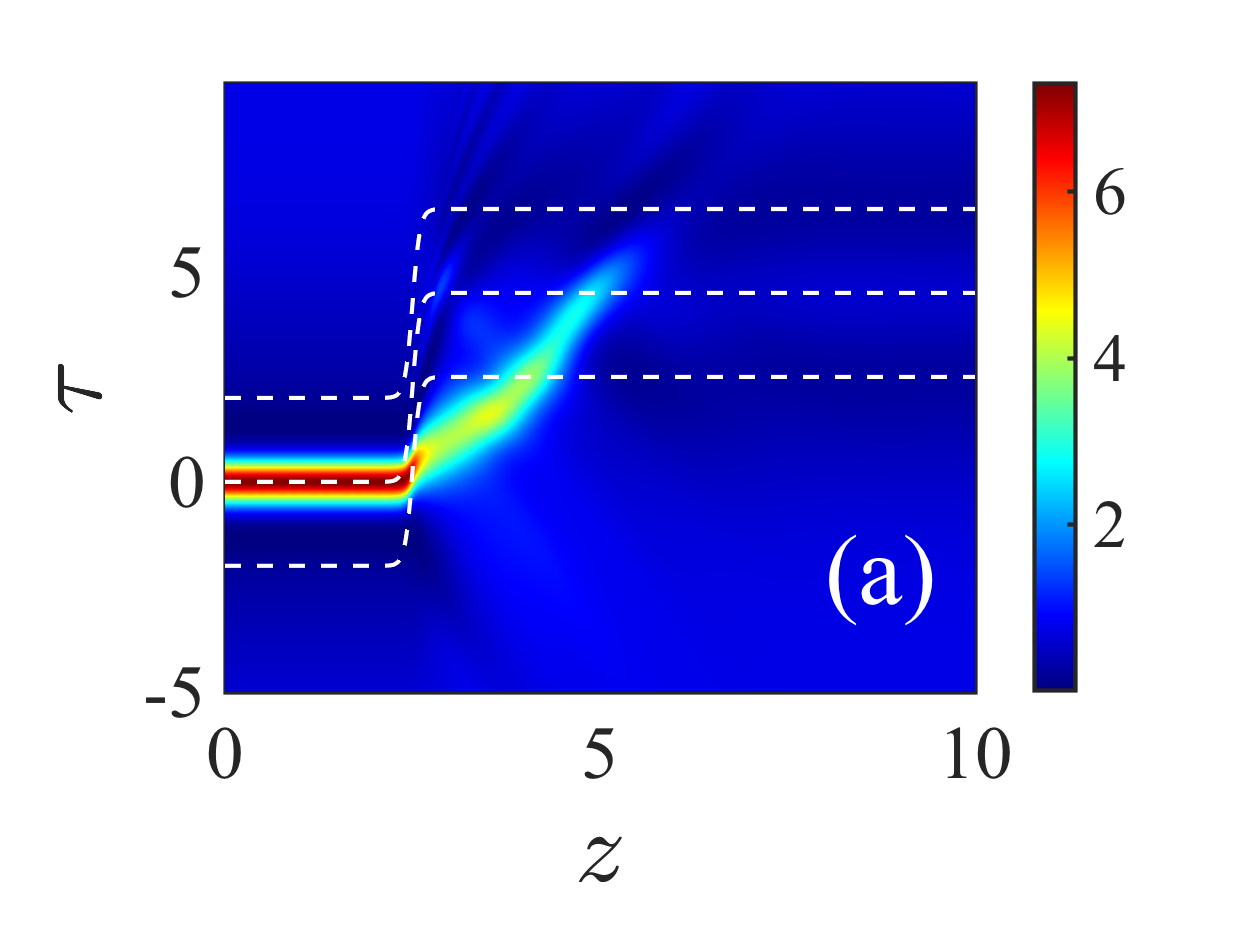
\includegraphics[width=4.2cm]{regularDensity5.eps} 
\hskip -0.5em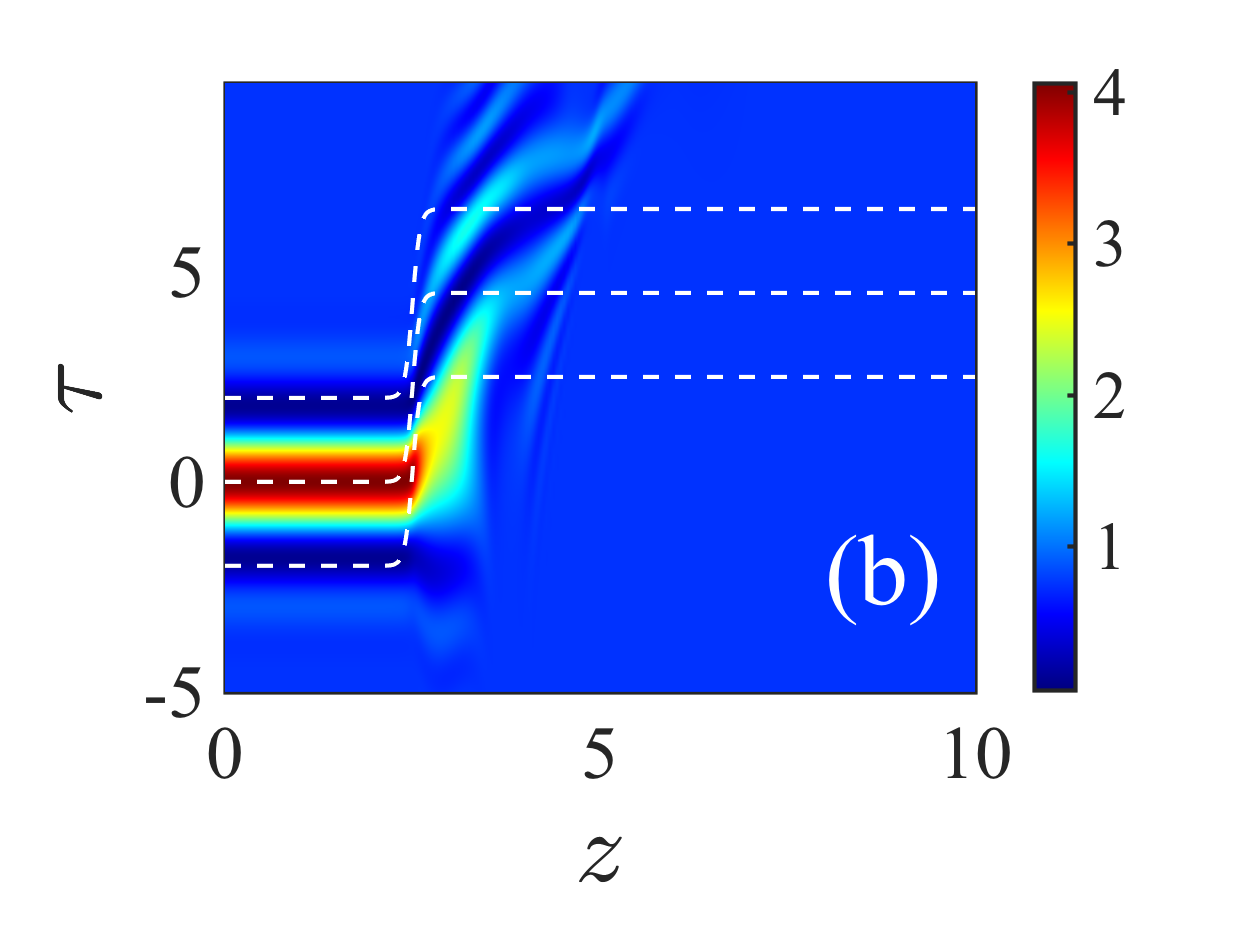
\includegraphics[width=4.2cm]{regularNCVADensity5.eps} 
\\
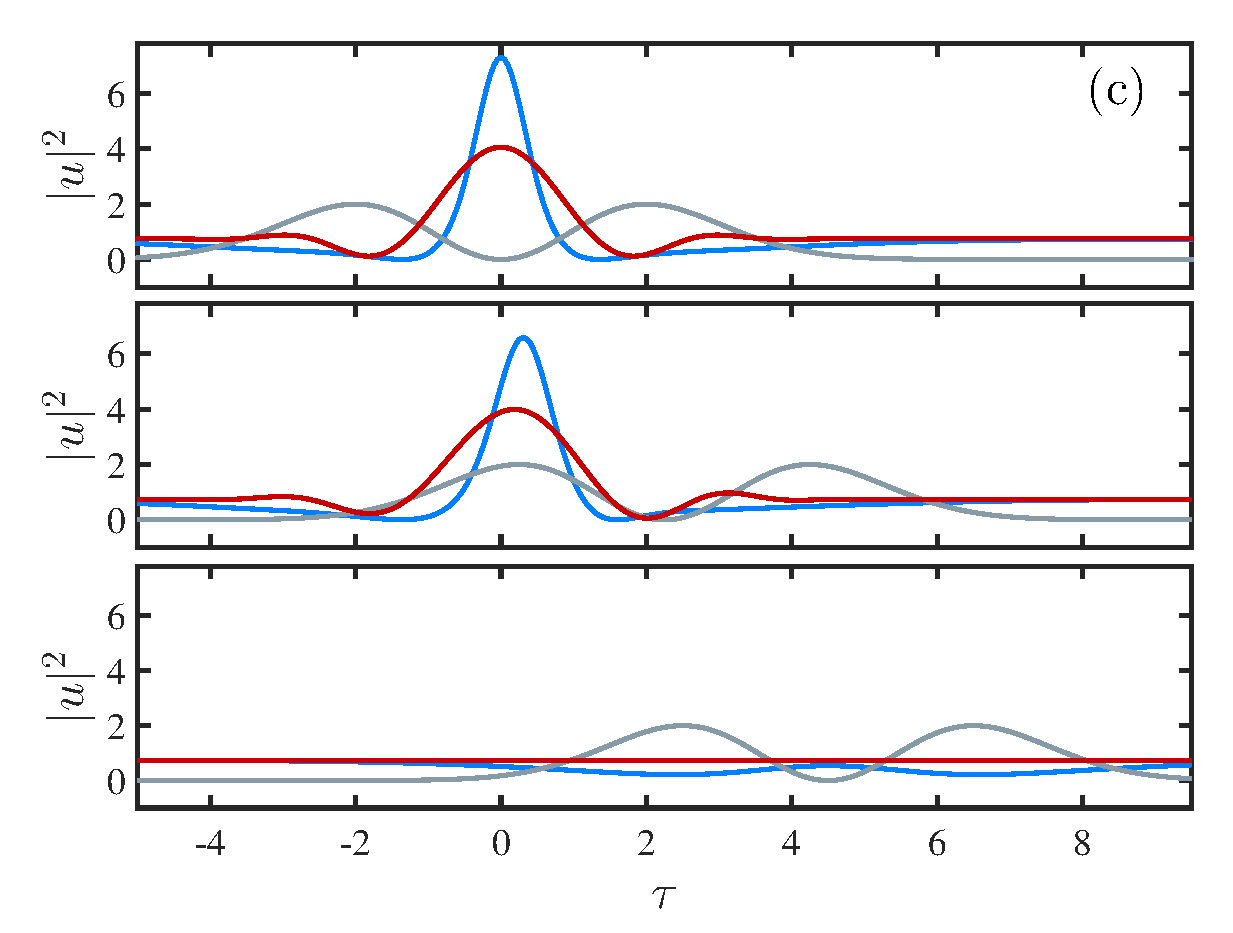
\includegraphics[width=8cm]{regularTimeSeries5.eps} 
\vspace{-0.5em}
\caption[Dynamic Evolution of Natural Tweezer with no-CS]{Dynamic evolution as in Fig.~\ref{fig:Regular1} but for $\tau_f = 4.5$ and $\beta = 10$.  Same layout as in Fig.~\ref{fig:Regular1}.  In this sample, the NCVA and LL solutions are both no-CS. 
}
\label{fig:Regular2}
\end{figure}
%%%%%%%%%% Fig  %%%%%%%%%%%%%%%%%%%%%%%%%%%%%%%%%%%%%%

%%%%%%%%%% Fig  %%%%%%%%%%%%%%%%%%%%%%%%%%%%%%%%%%%%%%
\begin{figure}[htb!]
\centering
\hskip 0.4em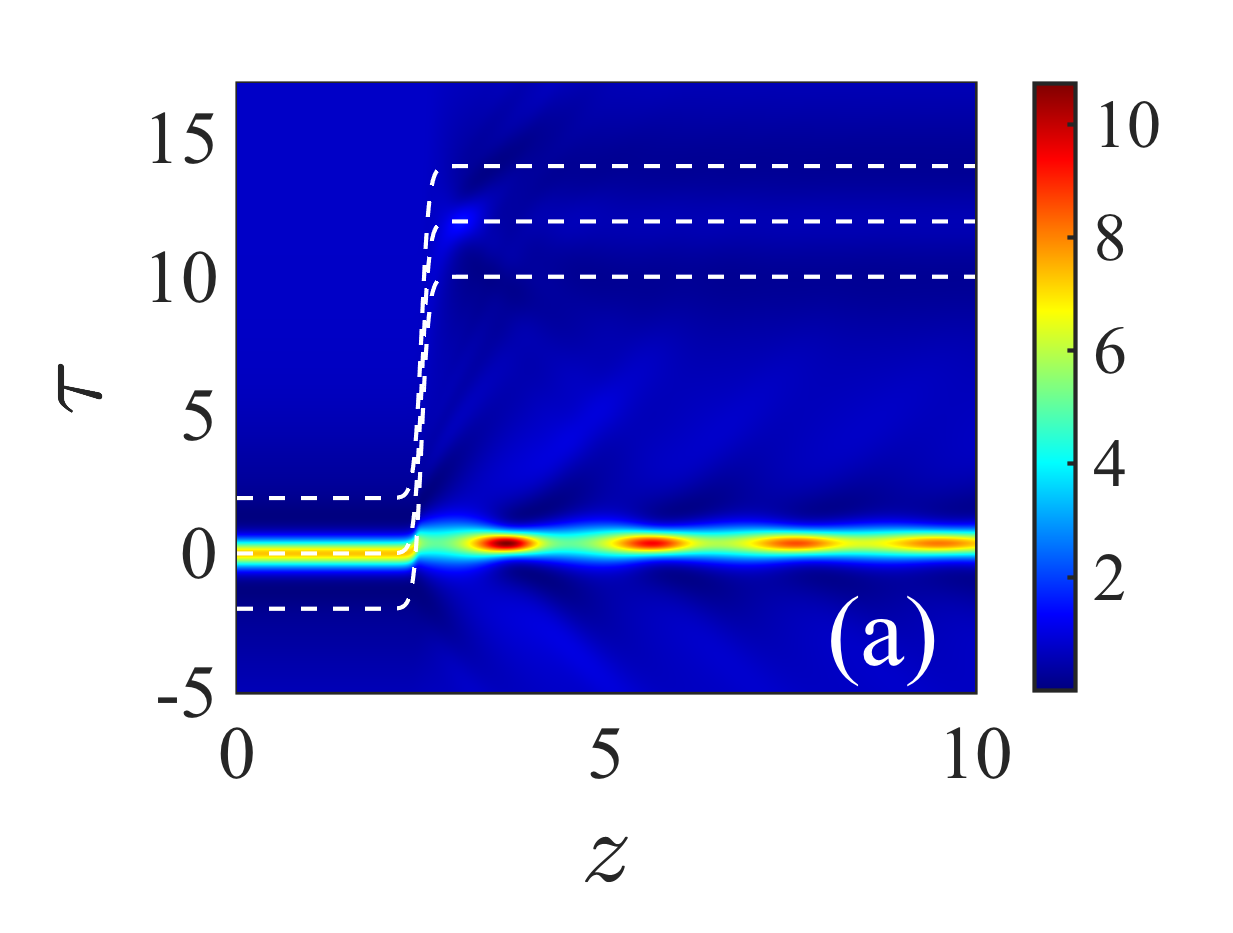
\includegraphics[width=4.2cm]{regularDensity3.eps} 
\hskip -0.5em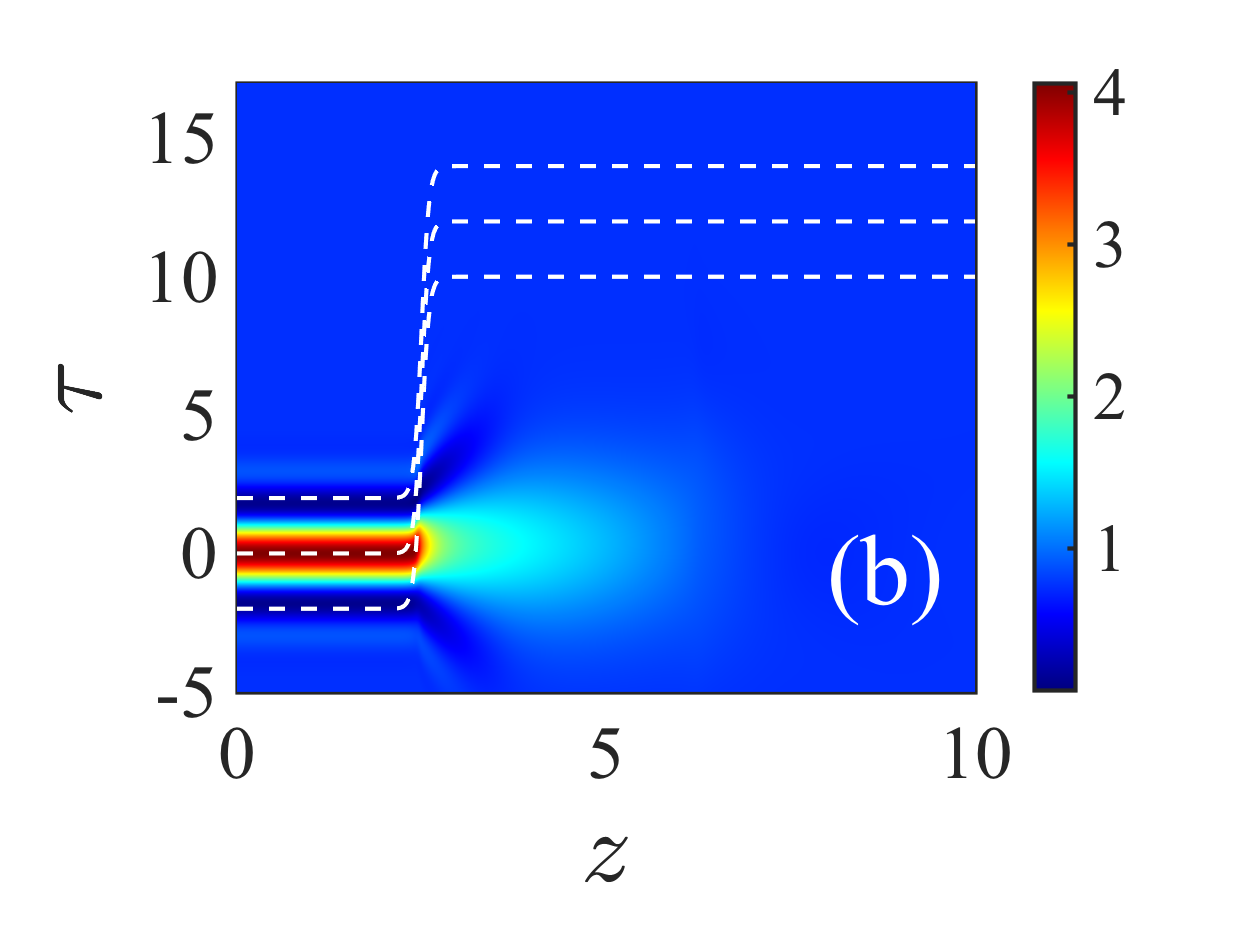
\includegraphics[width=4.2cm]{regularNCVADensity3.eps} 
\\
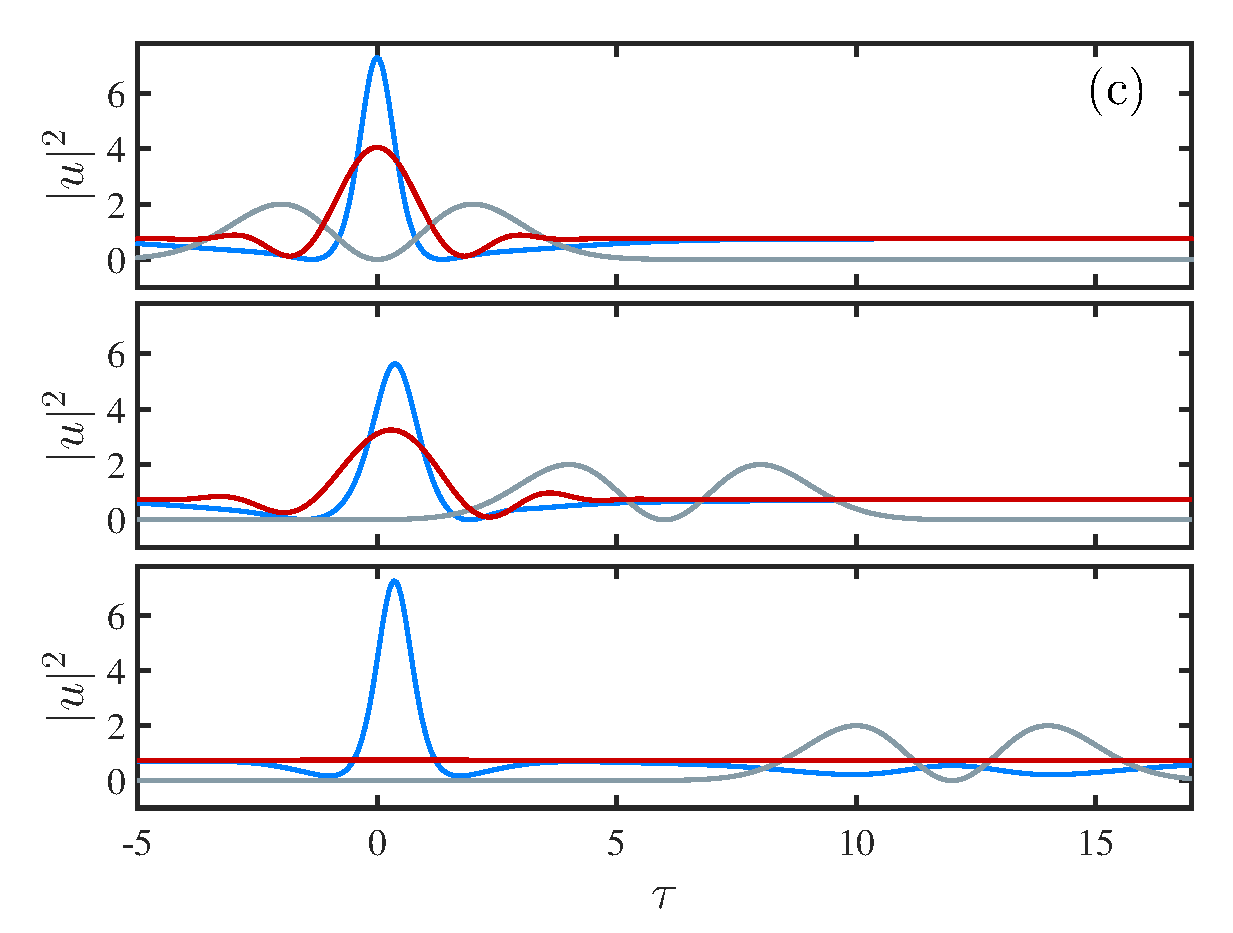
\includegraphics[width=8cm]{regularTimeSeries3.eps} 
\vspace{-0.5em}
\caption[Dynamic Evolution of Natural Tweezer with Non-Tweezed CS]{Dynamic evolution as in Fig.~\ref{fig:Regular1} but for $\tau_f = 12$ and $\beta = 10$.  Same layout as in Fig.~\ref{fig:Regular1}.  In this sample, the NCVA solution is a no-CS.  The CS of the LL model is stationary outside the natural width tweezer, which leaves the CS behind as the phase modulation is moved, referred to as a non-tweezed CS.
}
\label{fig:Regular3}
\end{figure}
%%%%%%%%%% Fig  %%%%%%%%%%%%%%%%%%%%%%%%%%%%%%%%%%%%%%

%%%%%%%%%% Fig  %%%%%%%%%%%%%%%%%%%%%%%%%%%%%%%%%%%%%%
\begin{figure}[htb!]
\centering
\hskip 0.4em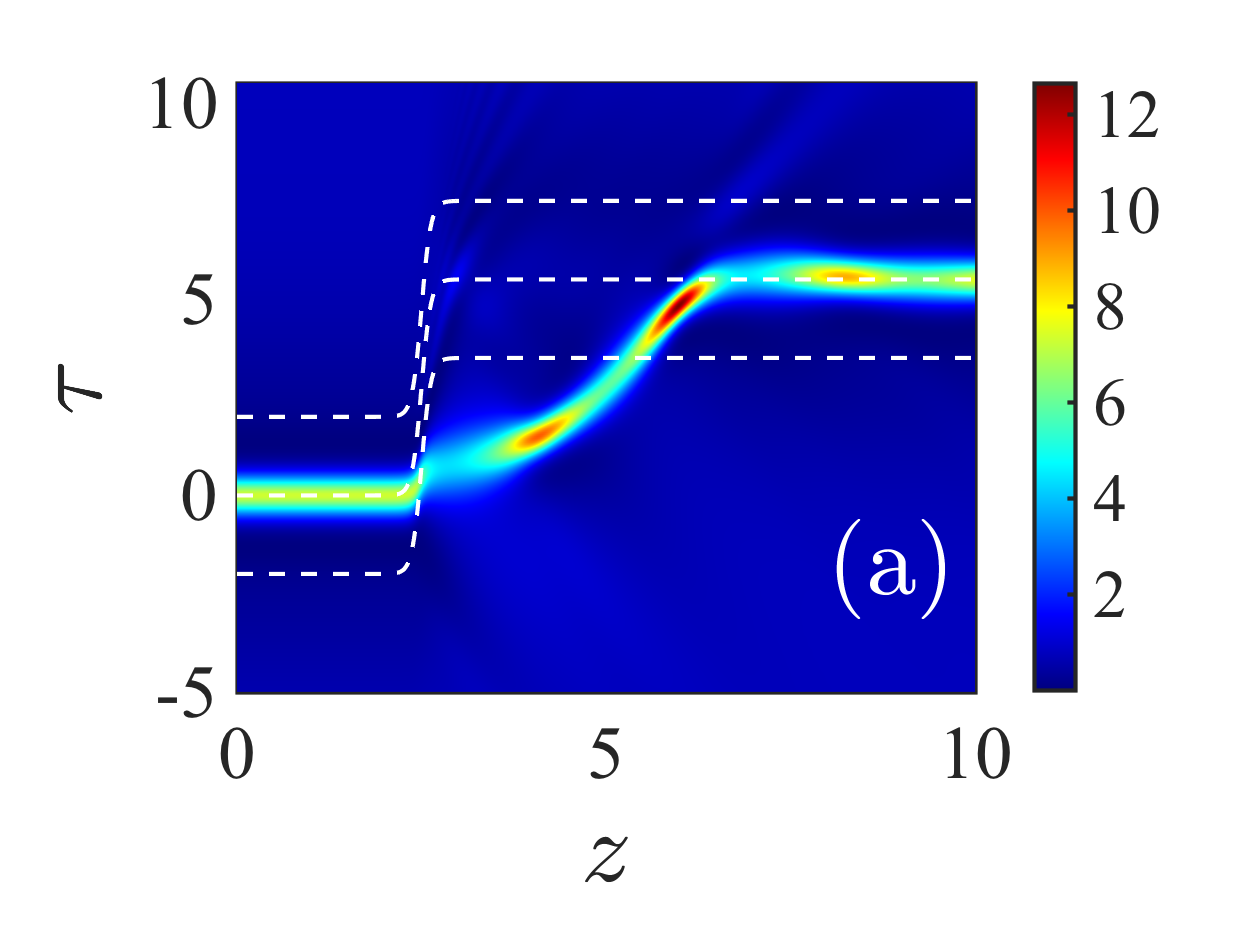
\includegraphics[width=4.2cm]{regularDensity6.eps} 
\hskip -0.5em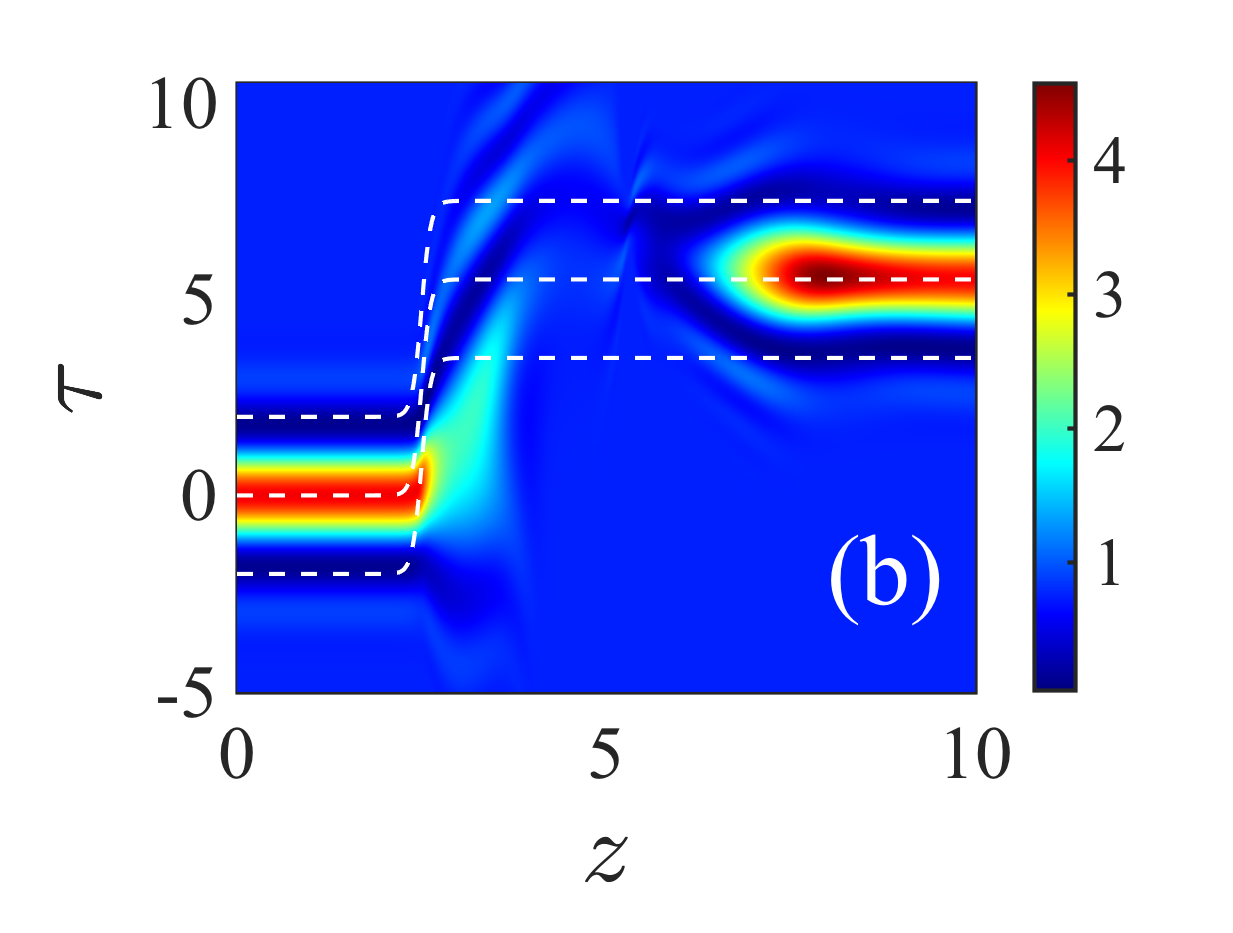
\includegraphics[width=4.2cm]{regularNCVADensity6.eps} 
\\
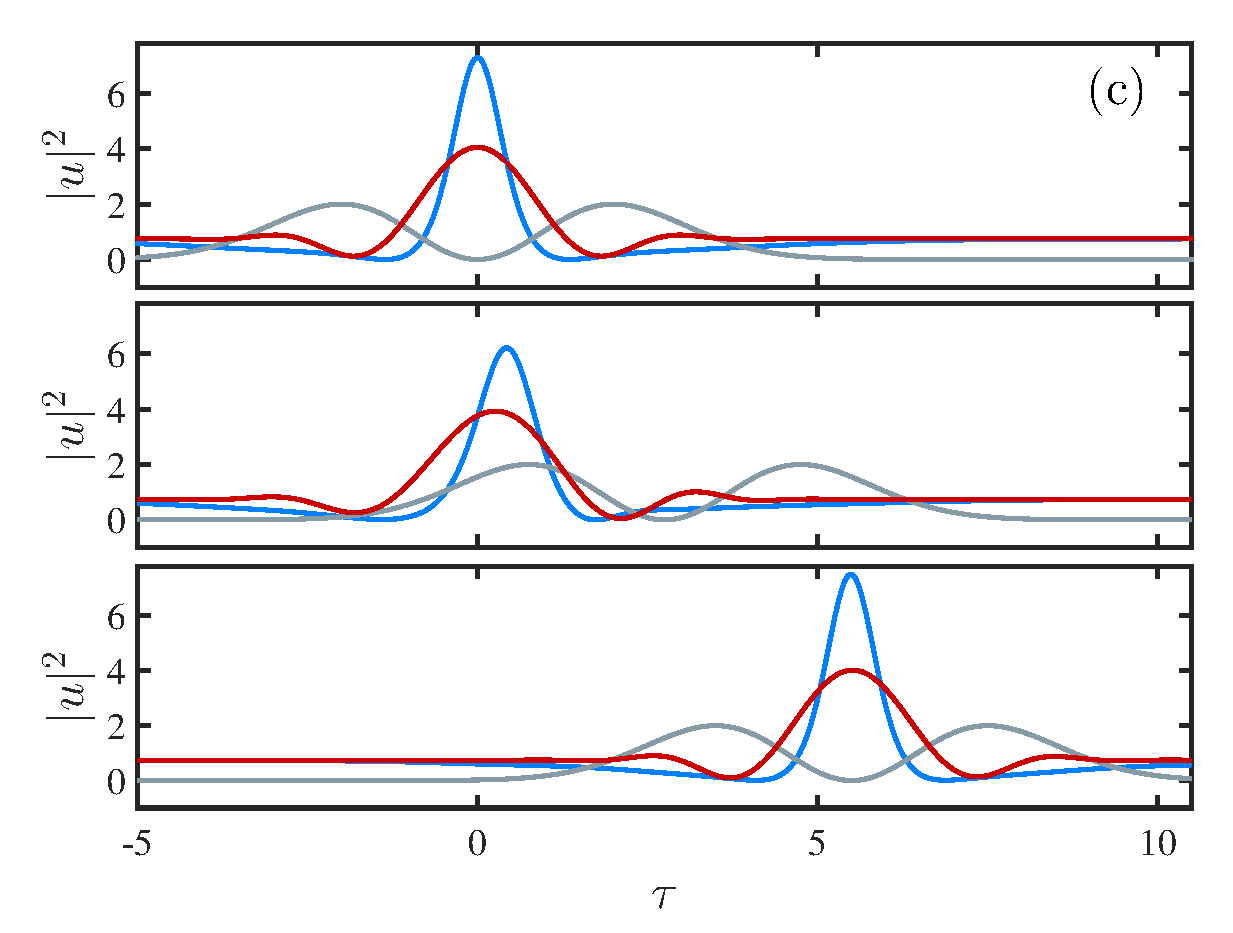
\includegraphics[width=8cm]{regularTimeSeries6.eps} 
\vspace{-0.5em}
\caption[Dynamic Evolution of Natural Tweezer with no-CS]{Dynamic evolution as in Fig.~\ref{fig:Regular1} but for $\tau_f = 5.5$ and $\beta = 8$.  Same layout as in Fig.~\ref{fig:Regular1}.   In this example, the LL model and NCVA has an ``artificially'' tweezed CS defined by the complete loss of the CS from the trap, but rather than a stationary CS left outside the trap (as is the case in non-tweezed CS), the CS is imparted with enough energy to continue moving in the direction of the tweezer.  By the final time $z_f$ the CS catches up with the tweezer and LL solutions and NCVA are both tweezed CS. 
}
\label{fig:Regular4}
\end{figure}
%%%%%%%%%% Fig  %%%%%%%%%%%%%%%%%%%%%%%%%%%%%%%%%%%%%%


As a sample of the dynamic properties of tweezability, Fig.~\ref{fig:Regular1} is a tweezed CS (blue region Fig.~\ref{fig:RegularQ}) for both the full LL model and the NCVA.  Fig.~\ref{fig:Regular2} is the no-CS solution  (green region Fig.~\ref{fig:RegularQ}).  For the third sample, Fig.~\ref{fig:Regular3} the tweezer leaves the CS outside the effective potential in the full LL model while in the NCVA the solution is dissipative (red region Fig.~\ref{fig:RegularQ}), which can not be captured by the NCVA.  In contrast, Fig.~\ref{fig:RegularQ} depicts the existence of an ``artificial'' tweezed CS solution for both the full LL model and the NCVA (blue inlet and island region, respectively in Fig.~\ref{fig:RegularQ}).  As Figs.~\ref{fig:Regular1}(a) and (b) show, the initial state [see solid (blue) line LL model solution and solid (red) line NCVA solution in Fig.~\ref{fig:Regular1}(c) top panel] is manipulated by the natural width tweezer towards $\tau_f$ at speed $\beta$ [see solid (blue) line LL model solution  and solid (red) line NCVA solution in Fig.~\ref{fig:Regular1}(c) bottom panel], which we refer to as a tweezed CS in both the LL model and NCVA.  Figures~\ref{fig:Regular2}(a) and (b) show the initial state [see solid (blue) line LL model solution and solid (red) line NCVA solution in Fig.~\ref{fig:Regular2}(c) top panel] and as the CS is dragged the solution dissipates until there is no longer a CS, in agreement between the LL model and NCVA  [see solid (blue) line LL model solution and solid (red) line NCVA solution in Fig.~\ref{fig:Regular2}(c) bottom panel].   As Figs.~\ref{fig:Regular3}(a) and (b) show the initial state [see solid (blue) line LL model solution and solid (red) line NCVA solution in Fig.~\ref{fig:Regular3}(c) top panel] is left behind as the natural tweezer is displaced for the LL model and is completely lost in the case of the NCVA  [see solid (blue) line LL model solution  and solid (red) line NCVA solution in Fig.~\ref{fig:Regular3}(c) bottom panel].  For the artificial tweezing dynamic properties, Figs.~\ref{fig:Regular4}(a) and (b) show the initial state [see solid (blue) line LL model solution and solid (red) line NCVA solution in Fig.~\ref{fig:Regular4}(c) top panel] is manipulated by the natural width tweezer towards $\tau_f$ at speed $\beta$ [see solid (blue) line LL model solution and solid (red) line NCVA solution in Fig.~\ref{fig:Regular4}(c) bottom panel], and as the CS is dragged the solution is initially lost, but catches back up and is re-trapped by the tweezer at $z_f$. 


Along with this example described here, Appendix~\ref{AppendixC} displays extra tweezers with (i) narrow width $h_\phi =2.3316$ and $\sigma_\phi$ = 1 in Sec.~\ref{section:Skinny} and (ii) wide width $h_\phi =6.9949$ and $\sigma_\phi$ = 3 in Sec.~\ref{section:Fat}.


\subsection{Demonstration of Temporal Tweezing}
 \label{section:FinalExample}
Next, we demonstrate the temporal tweezing of a trapped CS given our knowledge of parameter space $\tau_f$ and $\beta$.  Figure~\ref{fig:Final} is the dynamic properties of tweezability for both the full LL model and the NCVA with a natural width tweezer.  In Fig.~\ref{fig:Final}, instead of a single value of $\tau_f$ and $\beta$ we change the parameters at set increments of slow time $z$.  For $z\le5$, $\tau_f$=2 and $\beta$ = 10, then for $5 < z\le10$, $\tau_f$=0 and $\beta$ = 10, then for $10 < z\le15$, $\tau_f$=3 and $\beta$ = 0.5, then for $15 < z\le20$, $\tau_f$=1 and $\beta$ = 20, then for $20 < z\le25$, $\tau_f$=-2 and $\beta$ = 0.5.  The LL model [Fig.~\ref{fig:Final}(a)] and NCVA [Fig.~\ref{fig:Final}(b)] dynamics are in agreement with the expected tweezed-CS and also with each other.  In the NCVA, Fig.~\ref{fig:Final}(b) has an additional black line depicting the ansatz parameter $\xi$ which follows the center position of the tweezer $\tau_0$.  The example is designed to illustrate how the phase-modulation can move the trapped CS with different speeds at will.  
 
%%%%%%%%%% Fig  %%%%%%%%%%%%%%%%%%%%%%%%%%%%%%%%%%%%%%
\begin{figure*}[htb!]
\centering
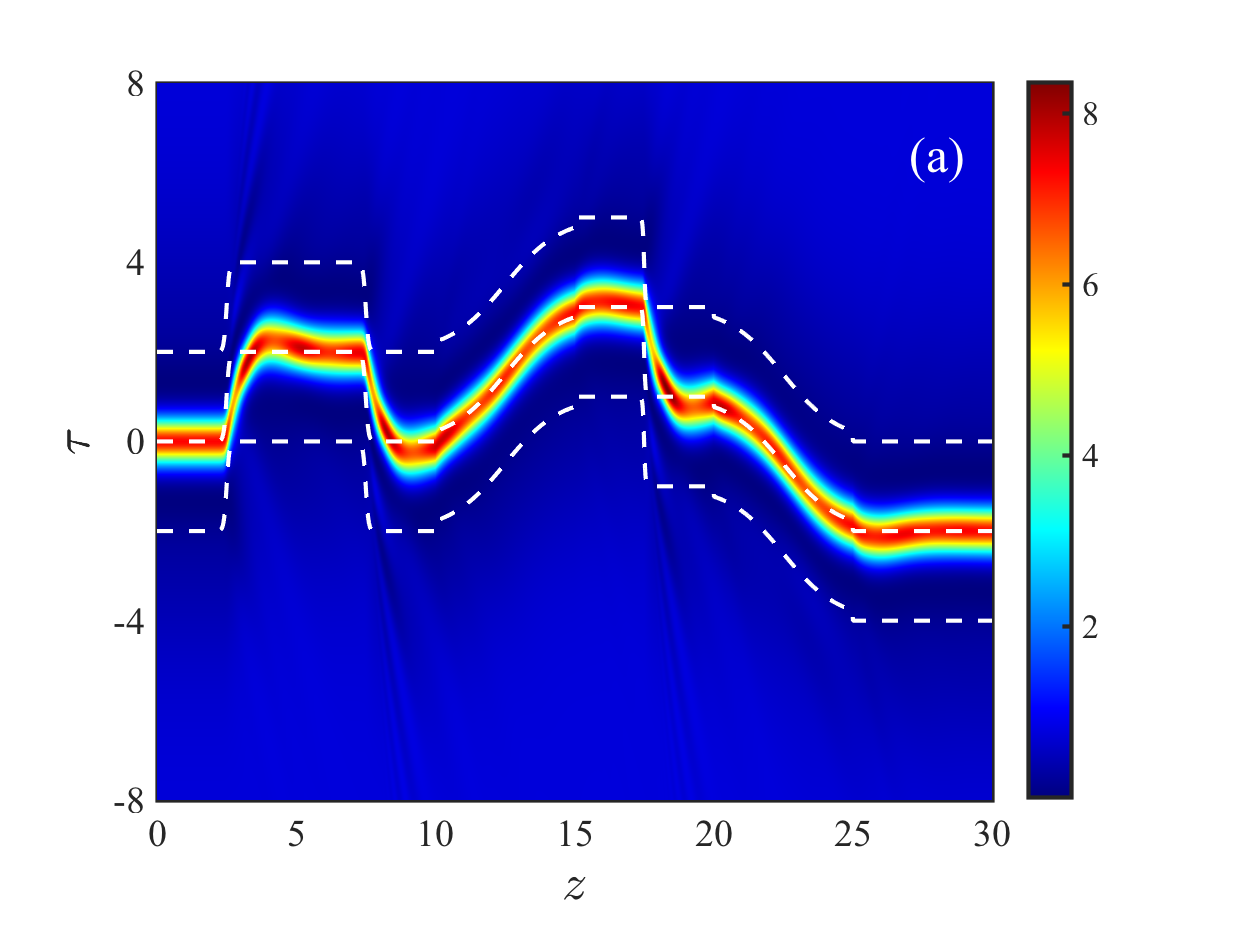
\includegraphics[width=8.8cm]{regularDensityFinal.eps} 
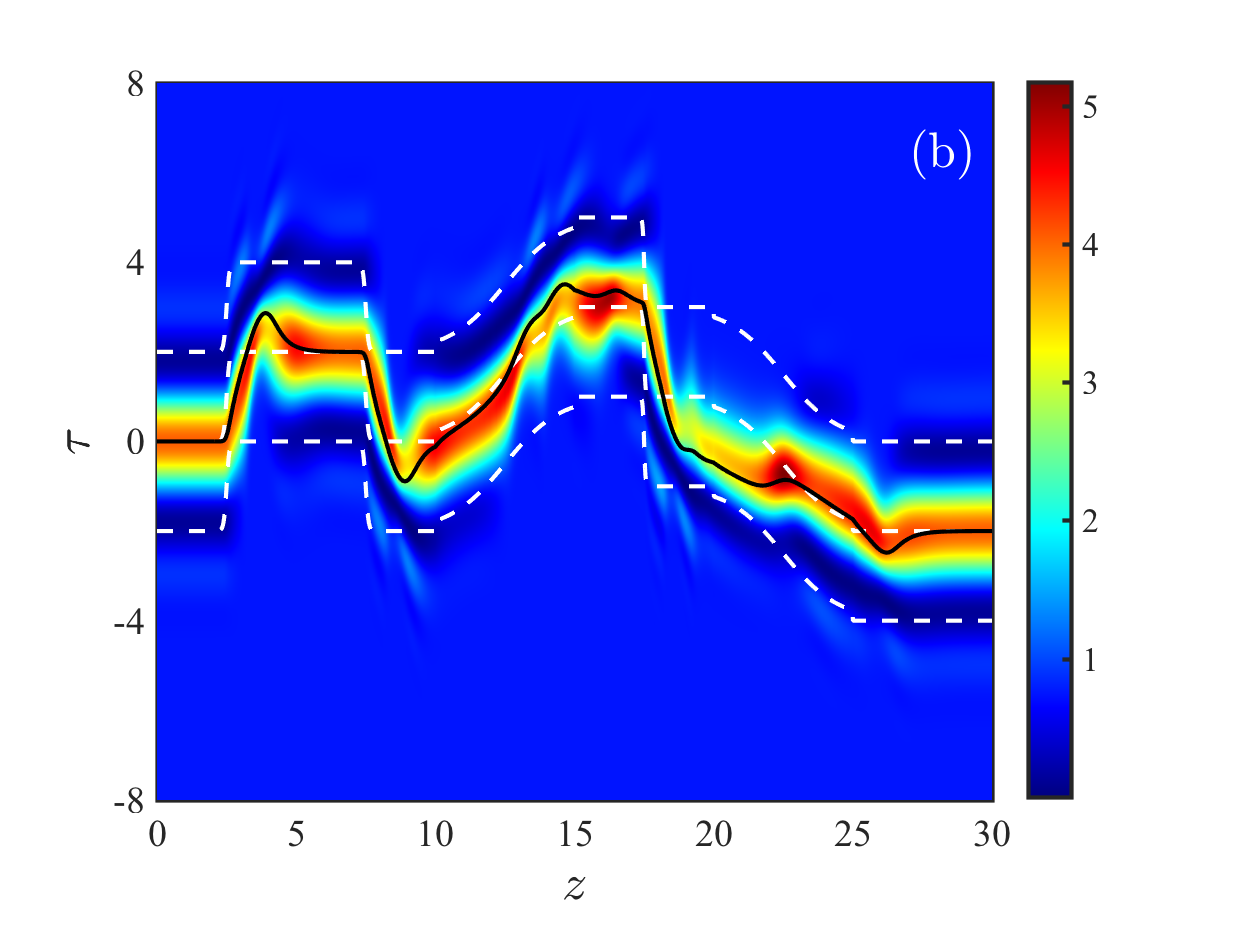
\includegraphics[width=8.8cm]{regularNCVADensityFinal.eps} 
\vspace{-0.5em}
\caption[Dynamic Evolution of Tweezed CS]{Dynamic evolution as in Fig.~\ref{fig:Regular1} but for variable $\tau_f$ and $\beta$.  Same layout as in Fig.~\ref{fig:Regular1}(a) and (b).  In this sample, we illustrate how a CS can be discretely manipulated given various parameters of $\tau_f$ and $\beta$.  The LL model (a) and NCVA (b) solution continues to be tweezed as the tweezer is moved at various speeds.  The dashed white lines are the center of $\tau_0(z)$ and $\pm \sigma_\phi$.  In panel (b) the black line is the NCVA variational parameter $\xi$.
}
\label{fig:Final}
\end{figure*}
%%%%%%%%%% Fig  %%%%%%%%%%%%%%%%%%%%%%%%%%%%%%%%%%%%%%

%%%%%%%%%%%%% Section: Conclusion
\section{Conclusions \& Future Challenges
\label{secConclusion}}
%In summary, we studied an LL equation modified to include a controllable temporal phase modulation introduced through $\phi(\tau, z)$ to describe temporal tweezing of CSs.  Our motivation was to understand when the parameters of the phase modulation were adequate to successfully tweeze the CS and when they failed.  We found thresholds for tweezing a CS dependent on the total displacement and the speed of the tweezer.  In our analysis, we also found that the shape of the tweezer impacts these regions and can have a dramatic effect on the dynamics of the CS.  In the full LL model there are three fundamental states: a tweezed CS, a non-tweezed CS and a no-CS. By contrast, the NCVA only describes two states: a tweezed CS and a no-CS.  .  The narrow tweezer is a bad candidate for tweezing, but the natural and wide width tweezers can give good control and manipulation of a CS.  .  Instead of full analysis of the LL model, we can use the NCVA to determine a lower bound on the threshold for phase modulation parameters where there exists temporal tweezing of a CS.  

We extend the NCVA approach to temporal cavity solitons which are stored in a passive loop of optical fiber pumped by a continuous-wave laser beam and observed in Ref.~\cite{tweeze} to be temporally tweezed through phase-modulation of the holding beam.  Temporal tweezing is modeled by the LL equation with additional terms due to the incorporation of a tweezer in the holding beam.  In our study, we assume a Gaussian phase-modulation and find the existence of three dynamical states (depending on the tweezer parameters) namely, a tweezed CS, a non-tweezed CS, and a dissipative CS.  We also develop a Lagrangian for the modified LL equation and its application to the NCVA.  The NCVA is capable of predicting the threshold in the tweezer parameter space for tweezed CSs and dissipative no-CS states---although it is not adequate for fully capturing more complex dynamics (especially so for tweezers with large displacements and speeds).  From our analysis of temporal tweezing, we have beneficial insight into the design of tweezers used in optical information processing, which requires the ability to trap ultrashort pulses of light and dynamically move them around in time, with respect to, and independently of other pulses of light.
%

In reference to temporal tweezing, multiple CSs can be present simultaneously and independently at arbitrary locations in a passive loop of optical fiber.  Therefore, a very interesting extension would be to add interactions of multiple CSs in the system.  Investigating the dynamics, interactions, and tweezability of the CS by allowing for long-range soliton interactions is necessary to understand an effective treatment of a CS, each of which constitute an ideal bit in optical information processing.

A very interesting extension of the temporal tweezing study is to analyze the linearization spectrum of the system and identify the stability/instability transitions between the three states we identified.  In this same vein, the identification of the spectrum can be used with the Galerkin approach capable of capturing bifurcations induced by changing the speed of the tweezer.  From our study of the LL equation and NCVA, we have developed a process to identify regions of tweezability which can aid experimental design and reliability of temporal tweezing used for information processing.
 

%

%\begin{thebibliography}{99}
%\itemsep3pt
\bibliographystyle{aip}
\bibliography{references}
%\end{thebibliography}

\clearpage
\onecolumngrid
\appendix 
% Appendix Template
\setstretch{1.3}
\chapter{NCVA System of Equations for Temporal Tweezing of Cavity Soliton} % Main appendix title
\label{AppendixA} % Change X to a consecutive letter; for referencing thI_{\sigma} appendix elsewhere, use \ref{AppendixX}
\lhead{Appendix B. \emph{NCVA System of Equations}}
\setstretch{2}

In this Appendix, we present the resulting modified Euler-Lagrange equations of motion from the LL Eq.~(\ref{eq:LLETweeze}) for temporal tweezing based on the NCVA where the over-dot denotes derivative with respect to $z$.  For explicit integrals $I_a$, $I_b$, $I_c$, $I_d$, $I_{\sigma}$, and $I_{\xi}$ please see Appendix~\ref{AppendixB}.  To simplify the expressions we use the following substitutions:
\begin{align}
A= \sqrt {{\sigma}^{2}+{{ \sigma_{\phi}}}^{2}}, \\
B= \sqrt {{\sigma}^{2}+2\,{{ \sigma_{\phi}}}^{2}},\\
C = {{\rm e}^{-{\frac { \left( { \xi}-{ \tau_0} \right) ^{2}}{{\sigma}^{2}+{{ \sigma_{\phi}}}^{2}}}}},\\
D = {{\rm e}^{-{\frac {\left( { \xi}-{ \tau_0} \right) ^{2}}{{\sigma}^{2}+2\,{{ \sigma_{\phi}}}^{2}}}}}.
\end{align}


\begin{landscape}
\begin{align}\dot{a}=&\frac{1}{4{a}{\sigma}^{3}{\sqrt{\pi}}\left({\sigma}^{2}+2\,{{\sigma_{\phi}}}^{2}\right)^{9/2}}\,\Bigg[-64\,{a}^{2}d\,{\sigma}^{9}\sqrt{\pi}B{{\sigma_{\phi}}}^{2}-192\,{a}^{2}d\,{\sigma}^{7}\sqrt{\pi}B{{\sigma_{\phi}}}^{4}-256\,{a}^{2}d\,{\sigma}^{5}\sqrt{\pi}B{{\sigma_{\phi}}}^{6}\nonumber\\&-128\,{a}^{2}d\,{\sigma}^{3}\sqrt{\pi}B{{\sigma_{\phi}}}^{8}+48\,{\sigma}^{2}{I_{b}}\,B{{\sigma_{\phi}}}^{8}-16\,{I_{d}}\,B{\sigma}^{6}{{\sigma_{\phi}}}^{2}-48\,{I_{d}}\,B{\sigma}^{4}{{\sigma_{\phi}}}^{4}\nonumber\\&-64\,{I_{d}}\,B{\sigma}^{2}{{\sigma_{\phi}}}^{6}-4\,{\sigma}^{11}\sqrt{\pi}{a}^{2}B+24\,{\sigma}^{8}{I_{b}}\,B{{\sigma_{\phi}}}^{2}+72\,{\sigma}^{6}{I_{b}}\,B{{\sigma_{\phi}}}^{4}+96\,{\sigma}^{4}{I_{b}}\,B{{\sigma_{\phi}}}^{6}\nonumber\\&+3\,{\sigma}^{10}{I_{b}}\,B-2\,{I_{d}}\,B{\sigma}^{8}-32\,{I_{d}}\,B{{\sigma_{\phi}}}^{8}-224\,D{h_{\phi}}\,{{\sigma_{\phi}}}^{3}{\sigma}^{5}{a}^{2}\sqrt{2}\sqrt{\pi}{{\xi}}^{2}-80\,D{h_{\phi}}\,{\sigma_{\phi}}\,{\sigma}^{7}{a}^{2}\sqrt{2}\sqrt{\pi}{{\tau_0}}^{2}\nonumber\\&+16\,{\sigma}^{5}\sqrt{\pi}{a}^{2}D\sqrt{2}{h_{\phi}}\,{{\tau_0}}^{4}{\sigma_{\phi}}-128\,D{h_{\phi}}\,{{\sigma_{\phi}}}^{5}{\sigma}^{3}{a}^{2}\sqrt{2}\sqrt{\pi}{{\tau_0}}^{2}-80\,D{h_{\phi}}\,{\sigma_{\phi}}\,{\sigma}^{7}{a}^{2}\sqrt{2}\sqrt{\pi}{{\xi}}^{2}-224\,D{h_{\phi}}\,{{\sigma_{\phi}}}^{3}{\sigma}^{5}{a}^{2}\sqrt{2}\sqrt{\pi}{{\tau_0}}^{2}\nonumber\\&-128\,D{h_{\phi}}\,{{\sigma_{\phi}}}^{5}{\sigma}^{3}{a}^{2}\sqrt{2}\sqrt{\pi}{{\xi}}^{2}+16\,{\sigma}^{5}\sqrt{\pi}{a}^{2}D\sqrt{2}{h_{\phi}}\,{{\xi}}^{4}{\sigma_{\phi}}+448\,D{h_{\phi}}\,{{\sigma_{\phi}}}^{3}{\sigma}^{5}{a}^{2}\sqrt{2}\sqrt{\pi}{\tau_0}\,{\xi}-8\,{a}^{2}d\,{\sigma}^{11}\sqrt{\pi}B\nonumber\\&-32\,{\sigma}^{9}\sqrt{\pi}{a}^{2}B{{\sigma_{\phi}}}^{2}-96\,{\sigma}^{7}\sqrt{\pi}{a}^{2}B{{\sigma_{\phi}}}^{4}-128\,{\sigma}^{5}\sqrt{\pi}{a}^{2}B{{\sigma_{\phi}}}^{6}-64\,{\sigma}^{3}\sqrt{\pi}{a}^{2}B{{\sigma_{\phi}}}^{8}\nonumber\\&+240\,{{\sigma_{\phi}}}^{5}{\sigma}^{5}\sqrt{\pi}D\sqrt{2}{h_{\phi}}\,{a}^{2}+128\,{{\sigma_{\phi}}}^{7}{\sigma}^{3}\sqrt{\pi}D\sqrt{2}{h_{\phi}}\,{a}^{2}+28\,{\sigma_{\phi}}\,{\sigma}^{9}\sqrt{\pi}D\sqrt{2}{h_{\phi}}\,{a}^{2}+144\,{{\sigma_{\phi}}}^{3}{\sigma}^{7}\sqrt{\pi}D\sqrt{2}{h_{\phi}}\,{a}^{2}\nonumber\\&+256\,D{h_{\phi}}\,{{\sigma_{\phi}}}^{5}{\sigma}^{3}{a}^{2}\sqrt{2}\sqrt{\pi}{\tau_0}\,{\xi}-64\,{\sigma}^{5}\sqrt{\pi}{a}^{2}D\sqrt{2}{h_{\phi}}\,{{\xi}}^{3}{\tau_0}\,{\sigma_{\phi}}-64\,{\sigma}^{5}\sqrt{\pi}{a}^{2}D\sqrt{2}{h_{\phi}}\,{{\tau_0}}^{3}{\xi}\,{\sigma_{\phi}}+96\,{\sigma}^{5}\sqrt{\pi}{a}^{2}D\sqrt{2}{h_{\phi}}\,{{\tau_0}}^{2}{\sigma_{\phi}}\,{{\xi}}^{2}\nonumber\\&+160\,D{h_{\phi}}\,{\sigma_{\phi}}\,{\sigma}^{7}{a}^{2}\sqrt{2}\sqrt{\pi}{\tau_0}\,{\xi}\Bigg]
\end{align}

{\allowdisplaybreaks
\begin{align}\dot{b}=&-\frac{1}{8{a}^{2}{\sqrt{\pi}}{\sigma}^{2}\left({\sigma}^{2}+{{\sigma_{\phi}}}^{2}\right)^{9/2}{{\sigma_{\phi}}}\left({\sigma}^{2}+2\,{{\sigma_{\phi}}}^{2}\right)^{9/2}}\,\Bigg[6\,{\sigma}^{18}C{{h_{\phi}}}^{2}{a}^{2}\sqrt{\pi}B-8\,{\sigma}^{17}A{\sigma_{\phi}}\,c\,{I_{c}}\,B-96\,{\sigma}^{15}A{{\sigma_{\phi}}}^{3}c\,{I_{c}}\,B\nonumber\\&-496\,{\sigma}^{13}A{{\sigma_{\phi}}}^{5}c\,{I_{c}}\,B-1440\,{\sigma}^{11}A{{\sigma_{\phi}}}^{7}c\,{I_{c}}\,B-2568\,{\sigma}^{9}A{{\sigma_{\phi}}}^{9}c\,{I_{c}}\,B-2880\,{\sigma}^{7}A{{\sigma_{\phi}}}^{11}c\,{I_{c}}\,B\nonumber\\&+1488\,{\sigma}^{5}{{\sigma_{\phi}}}^{13}{I_{a}}\,ABa+2568\,{{\sigma_{\phi}}}^{9}{a}^{2}\sqrt{\pi}AB{\sigma}^{8}+2880\,{{\sigma_{\phi}}}^{11}{a}^{2}\sqrt{\pi}AB{\sigma}^{6}\nonumber\\&+1984\,{{\sigma_{\phi}}}^{13}{a}^{2}\sqrt{\pi}AB{\sigma}^{4}+768\,{{\sigma_{\phi}}}^{15}{a}^{2}\sqrt{\pi}AB{\sigma}^{2}+96\,AB{a}^{2}\sqrt{\pi}{{\sigma_{\phi}}}^{3}{\sigma}^{14}\nonumber\\&+496\,AB{a}^{2}\sqrt{\pi}{{\sigma_{\phi}}}^{5}{\sigma}^{12}+1440\,AB{a}^{2}\sqrt{\pi}{{\sigma_{\phi}}}^{7}{\sigma}^{10}+8\,{a}^{2}\sqrt{\pi}A{\sigma_{\phi}}\,B{\sigma}^{16}-1984\,{\sigma}^{5}{{\sigma_{\phi}}}^{13}Ac\,{I_{c}}\,B\nonumber\\&+576\,{\sigma}^{3}{{\sigma_{\phi}}}^{15}{I_{a}}\,ABa-768\,{\sigma}^{3}{{\sigma_{\phi}}}^{15}Ac\,{I_{c}}\,B+96\,{{\sigma_{\phi}}}^{17}{I_{a}}\,\sigma\,ABa\nonumber\\&-128\,{{\sigma_{\phi}}}^{17}\sigma\,Ac\,{I_{c}}\,B+6\,{\sigma}^{17}{I_{a}}\,A{\sigma_{\phi}}\,Ba+72\,{\sigma}^{15}{I_{a}}\,A{{\sigma_{\phi}}}^{3}Ba+372\,{\sigma}^{13}{I_{a}}\,A{{\sigma_{\phi}}}^{5}Ba\nonumber\\&+1080\,{\sigma}^{11}{I_{a}}\,A{{\sigma_{\phi}}}^{7}Ba+1926\,{\sigma}^{9}{I_{a}}\,A{{\sigma_{\phi}}}^{9}Ba+2160\,{\sigma}^{7}{I_{a}}\,A{{\sigma_{\phi}}}^{11}Ba\nonumber\\&-1536\,AB\left(\left|{v}\right|\right)^{2}{a}^{2}{\sigma}^{4}\sqrt{\pi}{{\sigma_{\phi}}}^{15}-5\,{a}^{4}\sqrt{2}\sqrt{\pi}{\sigma}^{18}A{\sigma_{\phi}}\,B-80\,{a}^{4}\sqrt{2}\sqrt{\pi}{\sigma}^{2}A{{\sigma_{\phi}}}^{17}B\nonumber\\&-60\,{a}^{4}\sqrt{2}\sqrt{\pi}{\sigma}^{16}A{{\sigma_{\phi}}}^{3}B-310\,{a}^{4}\sqrt{2}\sqrt{\pi}{\sigma}^{14}A{{\sigma_{\phi}}}^{5}B-900\,{a}^{4}\sqrt{2}\sqrt{\pi}{\sigma}^{12}A{{\sigma_{\phi}}}^{7}B\nonumber\\&-1605\,{a}^{4}\sqrt{2}\sqrt{\pi}{\sigma}^{10}A{{\sigma_{\phi}}}^{9}B-1800\,{a}^{4}\sqrt{2}\sqrt{\pi}{\sigma}^{8}A{{\sigma_{\phi}}}^{11}B-1240\,{a}^{4}\sqrt{2}\sqrt{\pi}{\sigma}^{6}A{{\sigma_{\phi}}}^{13}B\nonumber\\&-480\,{a}^{4}\sqrt{2}\sqrt{\pi}{\sigma}^{4}A{{\sigma_{\phi}}}^{15}B-128\,{{\sigma_{\phi}}}^{17}{a}^{2}{c}^{2}{\sigma}^{2}\sqrt{\pi}AB-768\,{\sigma}^{4}{{\sigma_{\phi}}}^{15}{a}^{2}{c}^{2}\sqrt{\pi}AB\nonumber\\&+384\,BC{{h_{\phi}}}^{2}{a}^{2}{\sigma}^{8}\sqrt{\pi}{{\sigma_{\phi}}}^{10}+96\,BC{{h_{\phi}}}^{2}{a}^{2}{\sigma}^{6}\sqrt{\pi}{{\sigma_{\phi}}}^{12}+60\,{\sigma}^{16}C{{h_{\phi}}}^{2}{a}^{2}\sqrt{\pi}B{{\sigma_{\phi}}}^{2}\nonumber\\&+246\,{\sigma}^{14}C{{h_{\phi}}}^{2}{a}^{2}\sqrt{\pi}B{{\sigma_{\phi}}}^{4}+528\,BC{{h_{\phi}}}^{2}{a}^{2}{\sigma}^{12}\sqrt{\pi}{{\sigma_{\phi}}}^{6}-4\,{\sigma}^{16}C{{h_{\phi}}}^{2}{a}^{2}\sqrt{\pi}B{{\tau_0}}^{2}\nonumber\\&-4\,{\sigma}^{16}C{{h_{\phi}}}^{2}{a}^{2}\sqrt{\pi}B{{\xi}}^{2}+624\,BC{{h_{\phi}}}^{2}{a}^{2}{\sigma}^{10}\sqrt{\pi}{{\sigma_{\phi}}}^{8}-384\,{\sigma}^{10}C{{h_{\phi}}}^{2}{{\sigma_{\phi}}}^{4}{a}^{2}\sqrt{\pi}B{{\tau_0}}^{2}{{\xi}}^{2}\nonumber\\&-1152\,{\sigma}^{8}C{{h_{\phi}}}^{2}{{\sigma_{\phi}}}^{6}{a}^{2}\sqrt{\pi}B{{\tau_0}}^{2}{{\xi}}^{2}-1536\,{\sigma}^{6}C{{h_{\phi}}}^{2}{{\sigma_{\phi}}}^{8}{a}^{2}\sqrt{\pi}B{{\tau_0}}^{2}{{\xi}}^{2}-768\,{\sigma}^{4}C{{h_{\phi}}}^{2}{{\sigma_{\phi}}}^{10}{a}^{2}\sqrt{\pi}B{{\tau_0}}^{2}{{\xi}}^{2}\nonumber\\&+32\,{\sigma}^{12}C{{h_{\phi}}}^{2}{{\sigma_{\phi}}}^{2}{a}^{2}\sqrt{\pi}B{{\tau_0}}^{3}{\xi}+256\,{\sigma}^{10}C{{h_{\phi}}}^{2}{{\sigma_{\phi}}}^{4}{a}^{2}\sqrt{\pi}B{{\tau_0}}^{3}{\xi}+1632\,BC{{h_{\phi}}}^{2}{{\sigma_{\phi}}}^{8}{\sigma}^{8}{a}^{2}\sqrt{\pi}{{\tau_0}}^{2}\nonumber\\&+1728\,BC{{h_{\phi}}}^{2}{{\sigma_{\phi}}}^{10}{\sigma}^{6}{a}^{2}\sqrt{\pi}{{\tau_0}}^{2}+832\,BC{{h_{\phi}}}^{2}{{\sigma_{\phi}}}^{12}{\sigma}^{4}{a}^{2}\sqrt{\pi}{{\tau_0}}^{2}+128\,BC{{h_{\phi}}}^{2}{{\sigma_{\phi}}}^{14}{\sigma}^{2}{a}^{2}\sqrt{\pi}{{\tau_0}}^{2}\nonumber\\&-8\,BC{{h_{\phi}}}^{2}{{\sigma_{\phi}}}^{2}{\sigma}^{14}{a}^{2}\sqrt{\pi}{{\xi}}^{2}+132\,BC{{h_{\phi}}}^{2}{{\sigma_{\phi}}}^{4}{\sigma}^{12}{a}^{2}\sqrt{\pi}{{\xi}}^{2}+832\,C{{h_{\phi}}}^{2}{{\sigma_{\phi}}}^{12}{a}^{2}\sqrt{\pi}{\sigma}^{4}B{{\xi}}^{2}\nonumber\\&+128\,C{{h_{\phi}}}^{2}{{\sigma_{\phi}}}^{14}{a}^{2}\sqrt{\pi}{\sigma}^{2}B{{\xi}}^{2}+8\,{\sigma}^{16}C{{h_{\phi}}}^{2}{a}^{2}\sqrt{\pi}B{\tau_0}\,{\xi}+744\,C{{h_{\phi}}}^{2}{{\sigma_{\phi}}}^{6}{a}^{2}\sqrt{\pi}{\sigma}^{10}B{{\xi}}^{2}\nonumber\\&+1632\,C{{h_{\phi}}}^{2}{{\sigma_{\phi}}}^{8}{a}^{2}\sqrt{\pi}{\sigma}^{8}B{{\xi}}^{2}+1728\,C{{h_{\phi}}}^{2}{{\sigma_{\phi}}}^{10}{a}^{2}\sqrt{\pi}{\sigma}^{6}B{{\xi}}^{2}-192\,{\sigma}^{8}C{{h_{\phi}}}^{2}{{\sigma_{\phi}}}^{6}{a}^{2}\sqrt{\pi}B{{\xi}}^{4}\nonumber\\&-256\,{\sigma}^{6}C{{h_{\phi}}}^{2}{{\sigma_{\phi}}}^{8}{a}^{2}\sqrt{\pi}B{{\xi}}^{4}-128\,{\sigma}^{4}C{{h_{\phi}}}^{2}{{\sigma_{\phi}}}^{10}{a}^{2}\sqrt{\pi}B{{\xi}}^{4}-8\,{\sigma}^{12}C{{h_{\phi}}}^{2}{{\sigma_{\phi}}}^{2}{a}^{2}\sqrt{\pi}B{{\tau_0}}^{4}\nonumber\\&-64\,{\sigma}^{10}C{{h_{\phi}}}^{2}{{\sigma_{\phi}}}^{4}{a}^{2}\sqrt{\pi}B{{\tau_0}}^{4}-192\,{\sigma}^{8}C{{h_{\phi}}}^{2}{{\sigma_{\phi}}}^{6}{a}^{2}\sqrt{\pi}B{{\tau_0}}^{4}-256\,{\sigma}^{6}C{{h_{\phi}}}^{2}{{\sigma_{\phi}}}^{8}{a}^{2}\sqrt{\pi}B{{\tau_0}}^{4}\nonumber\\&-128\,{\sigma}^{4}C{{h_{\phi}}}^{2}{{\sigma_{\phi}}}^{10}{a}^{2}\sqrt{\pi}B{{\tau_0}}^{4}-8\,{\sigma}^{12}C{{h_{\phi}}}^{2}{{\sigma_{\phi}}}^{2}{a}^{2}\sqrt{\pi}B{{\xi}}^{4}-64\,{\sigma}^{10}C{{h_{\phi}}}^{2}{{\sigma_{\phi}}}^{4}{a}^{2}\sqrt{\pi}B{{\xi}}^{4}\nonumber\\&-8\,BC{{h_{\phi}}}^{2}{{\sigma_{\phi}}}^{2}{\sigma}^{14}{a}^{2}\sqrt{\pi}{{\tau_0}}^{2}+132\,BC{{h_{\phi}}}^{2}{{\sigma_{\phi}}}^{4}{\sigma}^{12}{a}^{2}\sqrt{\pi}{{\tau_0}}^{2}\nonumber\\&+744\,BC{{h_{\phi}}}^{2}{{\sigma_{\phi}}}^{6}{\sigma}^{10}{a}^{2}\sqrt{\pi}{{\tau_0}}^{2}-48\,D{h_{\phi}}\,{{\sigma_{\phi}}}^{2}{a}^{2}d\,\sqrt{2}{\sigma}^{18}\sqrt{\pi}A-384\,D{h_{\phi}}\,{{\sigma_{\phi}}}^{4}{a}^{2}d\,\sqrt{2}{\sigma}^{16}\sqrt{\pi}A\nonumber\\&-1248\,D{h_{\phi}}\,{{\sigma_{\phi}}}^{6}{a}^{2}d\,\sqrt{2}{\sigma}^{14}\sqrt{\pi}A-2112\,D{h_{\phi}}\,{{\sigma_{\phi}}}^{8}{a}^{2}d\,\sqrt{2}{\sigma}^{12}\sqrt{\pi}A-1968\,D{h_{\phi}}\,{{\sigma_{\phi}}}^{10}{a}^{2}d\,\sqrt{2}{\sigma}^{10}\sqrt{\pi}A\nonumber\\&-960\,D{h_{\phi}}\,{{\sigma_{\phi}}}^{12}{a}^{2}d\,\sqrt{2}{\sigma}^{8}\sqrt{\pi}A-192\,D{h_{\phi}}\,{{\sigma_{\phi}}}^{14}{a}^{2}d\,\sqrt{2}{\sigma}^{6}\sqrt{\pi}A+1024\,{\sigma}^{6}C{{h_{\phi}}}^{2}{{\sigma_{\phi}}}^{8}{a}^{2}\sqrt{\pi}B{{\tau_0}}^{3}{\xi}\nonumber\\&+512\,{\sigma}^{4}C{{h_{\phi}}}^{2}{{\sigma_{\phi}}}^{10}{a}^{2}\sqrt{\pi}B{{\tau_0}}^{3}{\xi}+32\,{\sigma}^{12}C{{h_{\phi}}}^{2}{{\sigma_{\phi}}}^{2}{a}^{2}\sqrt{\pi}B{{\xi}}^{3}{\tau_0}+256\,{\sigma}^{10}C{{h_{\phi}}}^{2}{{\sigma_{\phi}}}^{4}{a}^{2}\sqrt{\pi}B{{\xi}}^{3}{\tau_0}\nonumber\\&+768\,{\sigma}^{8}C{{h_{\phi}}}^{2}{{\sigma_{\phi}}}^{6}{a}^{2}\sqrt{\pi}B{{\xi}}^{3}{\tau_0}+1024\,{\sigma}^{6}C{{h_{\phi}}}^{2}{{\sigma_{\phi}}}^{8}{a}^{2}\sqrt{\pi}B{{\xi}}^{3}{\tau_0}+512\,{\sigma}^{4}C{{h_{\phi}}}^{2}{{\sigma_{\phi}}}^{10}{a}^{2}\sqrt{\pi}B{{\xi}}^{3}{\tau_0}\nonumber\\&+16\,{\sigma}^{14}C{{h_{\phi}}}^{2}{a}^{2}\sqrt{\pi}B{\tau_0}\,{\xi}\,{{\sigma_{\phi}}}^{2}-264\,{\sigma}^{12}C{{h_{\phi}}}^{2}{a}^{2}\sqrt{\pi}B{\tau_0}\,{\xi}\,{{\sigma_{\phi}}}^{4}-1488\,{\sigma}^{10}C{{h_{\phi}}}^{2}{a}^{2}\sqrt{\pi}B{\tau_0}\,{\xi}\,{{\sigma_{\phi}}}^{6}\nonumber\\&-3264\,{\sigma}^{8}C{{h_{\phi}}}^{2}{a}^{2}\sqrt{\pi}B{\tau_0}\,{\xi}\,{{\sigma_{\phi}}}^{8}-3456\,BC{{h_{\phi}}}^{2}{{\sigma_{\phi}}}^{10}{\sigma}^{6}{a}^{2}\sqrt{\pi}{\tau_0}\,{\xi}-1664\,BC{{h_{\phi}}}^{2}{{\sigma_{\phi}}}^{12}{\sigma}^{4}{a}^{2}\sqrt{\pi}{\tau_0}\,{\xi}\nonumber\\&-256\,BC{{h_{\phi}}}^{2}{{\sigma_{\phi}}}^{14}{\sigma}^{2}{a}^{2}\sqrt{\pi}{\tau_0}\,{\xi}-48\,{\sigma}^{12}C{{h_{\phi}}}^{2}{{\sigma_{\phi}}}^{2}{a}^{2}\sqrt{\pi}B{{\tau_0}}^{2}{{\xi}}^{2}-1984\,{\sigma}^{6}{{\sigma_{\phi}}}^{13}{a}^{2}{c}^{2}\sqrt{\pi}AB\nonumber\\&-8\,{\sigma}^{18}{a}^{2}{c}^{2}\sqrt{\pi}A{\sigma_{\phi}}\,B-96\,{\sigma}^{16}{a}^{2}{c}^{2}\sqrt{\pi}A{{\sigma_{\phi}}}^{3}B-496\,{\sigma}^{14}{a}^{2}{c}^{2}\sqrt{\pi}A{{\sigma_{\phi}}}^{5}B\nonumber\\&-1440\,{\sigma}^{12}{a}^{2}{c}^{2}\sqrt{\pi}A{{\sigma_{\phi}}}^{7}B-2568\,{\sigma}^{10}{a}^{2}{c}^{2}\sqrt{\pi}A{{\sigma_{\phi}}}^{9}B-2880\,{\sigma}^{8}{a}^{2}{c}^{2}\sqrt{\pi}A{{\sigma_{\phi}}}^{11}B\nonumber\\&-256\,AB\left(\left|{v}\right|\right)^{2}{a}^{2}{\sigma}^{2}\sqrt{\pi}{{\sigma_{\phi}}}^{17}+8\,AB\Delta\,{a}^{2}{\sigma}^{18}\sqrt{\pi}{\sigma_{\phi}}+96\,AB\Delta\,{a}^{2}{\sigma}^{16}\sqrt{\pi}{{\sigma_{\phi}}}^{3}\nonumber\\&+496\,AB\Delta\,{a}^{2}{\sigma}^{14}\sqrt{\pi}{{\sigma_{\phi}}}^{5}+1440\,AB\Delta\,{a}^{2}{\sigma}^{12}\sqrt{\pi}{{\sigma_{\phi}}}^{7}+2568\,AB\Delta\,{a}^{2}{\sigma}^{10}\sqrt{\pi}{{\sigma_{\phi}}}^{9}\nonumber\\&+2880\,AB\Delta\,{a}^{2}{\sigma}^{8}\sqrt{\pi}{{\sigma_{\phi}}}^{11}+1984\,AB\Delta\,{a}^{2}{\sigma}^{6}\sqrt{\pi}{{\sigma_{\phi}}}^{13}+768\,AB\Delta\,{a}^{2}{\sigma}^{4}\sqrt{\pi}{{\sigma_{\phi}}}^{15}\nonumber\\&+128\,AB\Delta\,{a}^{2}{\sigma}^{2}\sqrt{\pi}{{\sigma_{\phi}}}^{17}-16\,AB\left(\left|{v}\right|\right)^{2}{a}^{2}{\sigma}^{18}\sqrt{\pi}{\sigma_{\phi}}\nonumber\\&-192\,AB\left(\left|{v}\right|\right)^{2}{a}^{2}{\sigma}^{16}\sqrt{\pi}{{\sigma_{\phi}}}^{3}-992\,AB\left(\left|{v}\right|\right)^{2}{a}^{2}{\sigma}^{14}\sqrt{\pi}{{\sigma_{\phi}}}^{5}-2880\,AB\left(\left|{v}\right|\right)^{2}{a}^{2}{\sigma}^{12}\sqrt{\pi}{{\sigma_{\phi}}}^{7}\nonumber\\&-5136\,AB\left(\left|{v}\right|\right)^{2}{a}^{2}{\sigma}^{10}\sqrt{\pi}{{\sigma_{\phi}}}^{9}-5760\,AB\left(\left|{v}\right|\right)^{2}{a}^{2}{\sigma}^{8}\sqrt{\pi}{{\sigma_{\phi}}}^{11}-3968\,AB\left(\left|{v}\right|\right)^{2}{a}^{2}{\sigma}^{6}\sqrt{\pi}{{\sigma_{\phi}}}^{13}\nonumber\\&+768\,{\sigma}^{8}C{{h_{\phi}}}^{2}{{\sigma_{\phi}}}^{6}{a}^{2}\sqrt{\pi}B{{\tau_0}}^{3}{\xi}-64\,{{\sigma_{\phi}}}^{12}{\sigma}^{4}Ac\,{h_{\phi}}\,\sqrt{\pi}D\sqrt{2}{a}^{2}{{\xi}}^{3}+64\,{{\sigma_{\phi}}}^{12}{\sigma}^{4}Ac\,{h_{\phi}}\,\sqrt{\pi}D\sqrt{2}{a}^{2}{{\tau_0}}^{3}\nonumber\\&-64\,{\sigma}^{14}D{h_{\phi}}\,{{\sigma_{\phi}}}^{2}{a}^{2}\sqrt{2}\sqrt{\pi}A{{\xi}}^{4}d-2112\,{\sigma}^{10}{{\sigma_{\phi}}}^{8}D{h_{\phi}}\,{a}^{2}\sqrt{2}\sqrt{\pi}A{\tau_0}\,c-1968\,{\sigma}^{8}{{\sigma_{\phi}}}^{10}D{h_{\phi}}\,{a}^{2}\sqrt{2}\sqrt{\pi}A{\tau_0}\,c\nonumber\\&-192\,{\sigma}^{12}{{\sigma_{\phi}}}^{4}Ac\,{h_{\phi}}\,\sqrt{\pi}D\sqrt{2}{a}^{2}{{\xi}}^{3}-448\,{\sigma}^{10}{{\sigma_{\phi}}}^{6}Ac\,{h_{\phi}}\,\sqrt{\pi}D\sqrt{2}{a}^{2}{{\xi}}^{3}-64\,{\sigma}^{6}D{h_{\phi}}\,{{\sigma_{\phi}}}^{10}{a}^{2}\sqrt{2}\sqrt{\pi}A{{\xi}}^{4}d\nonumber\\&+192\,D{h_{\phi}}\,{{\sigma_{\phi}}}^{2}{a}^{2}\sqrt{2}\sqrt{\pi}{\sigma}^{16}Ad\,{{\tau_0}}^{2}+1152\,D{h_{\phi}}\,{{\sigma_{\phi}}}^{4}{a}^{2}\sqrt{2}\sqrt{\pi}{\sigma}^{14}Ad\,{{\tau_0}}^{2}\nonumber\\&+2688\,D{h_{\phi}}\,{{\sigma_{\phi}}}^{6}{a}^{2}\sqrt{2}\sqrt{\pi}{\sigma}^{12}Ad\,{{\tau_0}}^{2}+3072\,D{h_{\phi}}\,{{\sigma_{\phi}}}^{8}{a}^{2}\sqrt{2}\sqrt{\pi}{\sigma}^{10}Ad\,{{\tau_0}}^{2}+1728\,D{h_{\phi}}\,{{\sigma_{\phi}}}^{10}{a}^{2}\sqrt{2}\sqrt{\pi}{\sigma}^{8}Ad\,{{\tau_0}}^{2}\nonumber\\&+384\,D{h_{\phi}}\,{{\sigma_{\phi}}}^{12}{a}^{2}\sqrt{2}\sqrt{\pi}{\sigma}^{6}Ad\,{{\tau_0}}^{2}+1248\,{\sigma}^{12}{{\sigma_{\phi}}}^{6}D{h_{\phi}}\,{a}^{2}\sqrt{2}\sqrt{\pi}A{\xi}\,c+2112\,{\sigma}^{10}{{\sigma_{\phi}}}^{8}D{h_{\phi}}\,{a}^{2}\sqrt{2}\sqrt{\pi}A{\xi}\,c\nonumber\\&+1968\,{\sigma}^{8}{{\sigma_{\phi}}}^{10}D{h_{\phi}}\,{a}^{2}\sqrt{2}\sqrt{\pi}A{\xi}\,c+2688\,{\sigma}^{12}{{\sigma_{\phi}}}^{6}D{h_{\phi}}\,{a}^{2}\sqrt{2}\sqrt{\pi}Ad\,{{\xi}}^{2}+3072\,{\sigma}^{10}{{\sigma_{\phi}}}^{8}D{h_{\phi}}\,{a}^{2}\sqrt{2}\sqrt{\pi}Ad\,{{\xi}}^{2}\nonumber\\&+1728\,{\sigma}^{8}{{\sigma_{\phi}}}^{10}D{h_{\phi}}\,{a}^{2}\sqrt{2}\sqrt{\pi}Ad\,{{\xi}}^{2}-1248\,{\sigma}^{12}{{\sigma_{\phi}}}^{6}D{h_{\phi}}\,{a}^{2}\sqrt{2}\sqrt{\pi}A{\tau_0}\,c-256\,{\sigma}^{12}D{h_{\phi}}\,{{\sigma_{\phi}}}^{4}{a}^{2}\sqrt{2}\sqrt{\pi}A{{\tau_0}}^{4}d\nonumber\\&-384\,{\sigma}^{10}D{h_{\phi}}\,{{\sigma_{\phi}}}^{6}{a}^{2}\sqrt{2}\sqrt{\pi}A{{\tau_0}}^{4}d-256\,{\sigma}^{8}D{h_{\phi}}\,{{\sigma_{\phi}}}^{8}{a}^{2}\sqrt{2}\sqrt{\pi}A{{\tau_0}}^{4}d-64\,{\sigma}^{6}D{h_{\phi}}\,{{\sigma_{\phi}}}^{10}{a}^{2}\sqrt{2}\sqrt{\pi}A{{\tau_0}}^{4}d\nonumber\\&+192\,D{h_{\phi}}\,{{\sigma_{\phi}}}^{2}{a}^{2}\sqrt{2}\sqrt{\pi}{\sigma}^{16}Ad\,{{\xi}}^{2}+1152\,D{h_{\phi}}\,{{\sigma_{\phi}}}^{4}{a}^{2}\sqrt{2}\sqrt{\pi}{\sigma}^{14}Ad\,{{\xi}}^{2}-288\,{\sigma}^{6}{{\sigma_{\phi}}}^{10}Ac\,{h_{\phi}}\,\sqrt{\pi}D\sqrt{2}{a}^{2}{{\xi}}^{3}\nonumber\\&+288\,{\sigma}^{6}{{\sigma_{\phi}}}^{10}Ac\,{h_{\phi}}\,\sqrt{\pi}D\sqrt{2}{a}^{2}{{\tau_0}}^{3}+192\,{{\sigma_{\phi}}}^{14}D{h_{\phi}}\,{\sigma}^{4}{a}^{2}\sqrt{2}\sqrt{\pi}A{\xi}\,c-192\,{{\sigma_{\phi}}}^{14}D{h_{\phi}}\,{\sigma}^{4}{a}^{2}\sqrt{2}\sqrt{\pi}A{\tau_0}\,c\nonumber\\&-64\,{\sigma}^{14}D{h_{\phi}}\,{{\sigma_{\phi}}}^{2}{a}^{2}\sqrt{2}\sqrt{\pi}A{{\tau_0}}^{4}d-512\,{\sigma}^{8}{{\sigma_{\phi}}}^{8}Ac\,{h_{\phi}}\,\sqrt{\pi}D\sqrt{2}{a}^{2}{{\xi}}^{3}+192\,{\sigma}^{12}{{\sigma_{\phi}}}^{4}Ac\,{h_{\phi}}\,\sqrt{\pi}D\sqrt{2}{a}^{2}{{\tau_0}}^{3}\nonumber\\&+448\,{\sigma}^{10}{{\sigma_{\phi}}}^{6}Ac\,{h_{\phi}}\,\sqrt{\pi}D\sqrt{2}{a}^{2}{{\tau_0}}^{3}+512\,{\sigma}^{8}{{\sigma_{\phi}}}^{8}Ac\,{h_{\phi}}\,\sqrt{\pi}D\sqrt{2}{a}^{2}{{\tau_0}}^{3}+960\,{\sigma}^{6}{{\sigma_{\phi}}}^{12}D{h_{\phi}}\,{a}^{2}\sqrt{2}\sqrt{\pi}A{\xi}\,c\nonumber\\&+384\,{\sigma}^{6}{{\sigma_{\phi}}}^{12}D{h_{\phi}}\,{a}^{2}\sqrt{2}\sqrt{\pi}Ad\,{{\xi}}^{2}-960\,{\sigma}^{6}{{\sigma_{\phi}}}^{12}D{h_{\phi}}\,{a}^{2}\sqrt{2}\sqrt{\pi}A{\tau_0}\,c-32\,{\sigma}^{14}A{{\sigma_{\phi}}}^{2}c\,{h_{\phi}}\,\sqrt{\pi}D\sqrt{2}{a}^{2}{{\xi}}^{3}\nonumber\\&+32\,{\sigma}^{14}A{{\sigma_{\phi}}}^{2}c\,{h_{\phi}}\,\sqrt{\pi}D\sqrt{2}{a}^{2}{{\tau_0}}^{3}+48\,{\sigma}^{16}D{h_{\phi}}\,{{\sigma_{\phi}}}^{2}{a}^{2}\sqrt{2}\sqrt{\pi}A{\xi}\,c+384\,{\sigma}^{14}D{h_{\phi}}\,{{\sigma_{\phi}}}^{4}{a}^{2}\sqrt{2}\sqrt{\pi}A{\xi}\,c\nonumber\\&-48\,{\sigma}^{16}D{h_{\phi}}\,{{\sigma_{\phi}}}^{2}{a}^{2}\sqrt{2}\sqrt{\pi}A{\tau_0}\,c-384\,{\sigma}^{14}D{h_{\phi}}\,{{\sigma_{\phi}}}^{4}{a}^{2}\sqrt{2}\sqrt{\pi}A{\tau_0}\,c-256\,{\sigma}^{12}D{h_{\phi}}\,{{\sigma_{\phi}}}^{4}{a}^{2}\sqrt{2}\sqrt{\pi}A{{\xi}}^{4}d\nonumber\\&-384\,{\sigma}^{10}D{h_{\phi}}\,{{\sigma_{\phi}}}^{6}{a}^{2}\sqrt{2}\sqrt{\pi}A{{\xi}}^{4}d-256\,{\sigma}^{8}D{h_{\phi}}\,{{\sigma_{\phi}}}^{8}{a}^{2}\sqrt{2}\sqrt{\pi}A{{\xi}}^{4}d+1024\,{\sigma}^{12}D{h_{\phi}}\,{{\sigma_{\phi}}}^{4}{a}^{2}\sqrt{2}\sqrt{\pi}A{{\xi}}^{3}d\,{\tau_0}\nonumber\\&+1536\,{\sigma}^{10}D{h_{\phi}}\,{{\sigma_{\phi}}}^{6}{a}^{2}\sqrt{2}\sqrt{\pi}A{{\xi}}^{3}d\,{\tau_0}+1024\,{\sigma}^{8}D{h_{\phi}}\,{{\sigma_{\phi}}}^{8}{a}^{2}\sqrt{2}\sqrt{\pi}A{{\xi}}^{3}d\,{\tau_0}+256\,{\sigma}^{6}D{h_{\phi}}\,{{\sigma_{\phi}}}^{10}{a}^{2}\sqrt{2}\sqrt{\pi}A{{\xi}}^{3}d\,{\tau_0}\nonumber\\&+576\,{\sigma}^{12}A{{\sigma_{\phi}}}^{4}c\,{h_{\phi}}\,\sqrt{\pi}D\sqrt{2}{a}^{2}{\tau_0}\,{{\xi}}^{2}-96\,{\sigma}^{14}A{{\sigma_{\phi}}}^{2}c\,{h_{\phi}}\,\sqrt{\pi}D\sqrt{2}{a}^{2}{{\tau_0}}^{2}{\xi}\nonumber\\&-576\,{\sigma}^{12}A{{\sigma_{\phi}}}^{4}c\,{h_{\phi}}\,\sqrt{\pi}D\sqrt{2}{a}^{2}{{\tau_0}}^{2}{\xi}-384\,{\sigma}^{14}D{h_{\phi}}\,{{\sigma_{\phi}}}^{2}{a}^{2}\sqrt{2}\sqrt{\pi}A{{\tau_0}}^{2}{{\xi}}^{2}d-1536\,{\sigma}^{12}D{h_{\phi}}\,{{\sigma_{\phi}}}^{4}{a}^{2}\sqrt{2}\sqrt{\pi}A{{\tau_0}}^{2}{{\xi}}^{2}d\nonumber\\&-2304\,{\sigma}^{10}D{h_{\phi}}\,{{\sigma_{\phi}}}^{6}{a}^{2}\sqrt{2}\sqrt{\pi}A{{\tau_0}}^{2}{{\xi}}^{2}d-1536\,{\sigma}^{8}D{h_{\phi}}\,{{\sigma_{\phi}}}^{8}{a}^{2}\sqrt{2}\sqrt{\pi}A{{\tau_0}}^{2}{{\xi}}^{2}d-384\,{\sigma}^{6}D{h_{\phi}}\,{{\sigma_{\phi}}}^{10}{a}^{2}\sqrt{2}\sqrt{\pi}A{{\tau_0}}^{2}{{\xi}}^{2}d\nonumber\\&+1344\,{\sigma}^{10}{{\sigma_{\phi}}}^{6}Ac\,{h_{\phi}}\,\sqrt{\pi}D\sqrt{2}{a}^{2}{\tau_0}\,{{\xi}}^{2}-864\,{\sigma}^{6}{{\sigma_{\phi}}}^{10}Ac\,{h_{\phi}}\,\sqrt{\pi}D\sqrt{2}{a}^{2}{{\tau_0}}^{2}{\xi}+192\,{{\sigma_{\phi}}}^{12}{\sigma}^{4}Ac\,{h_{\phi}}\,\sqrt{\pi}D\sqrt{2}{a}^{2}{\tau_0}\,{{\xi}}^{2}\nonumber\\&-192\,{{\sigma_{\phi}}}^{12}{\sigma}^{4}Ac\,{h_{\phi}}\,\sqrt{\pi}D\sqrt{2}{a}^{2}{{\tau_0}}^{2}{\xi}-384\,{\sigma}^{16}D{h_{\phi}}\,{{\sigma_{\phi}}}^{2}{a}^{2}\sqrt{2}\sqrt{\pi}A{\xi}\,d\,{\tau_0}+96\,{\sigma}^{14}A{{\sigma_{\phi}}}^{2}c\,{h_{\phi}}\,\sqrt{\pi}D\sqrt{2}{a}^{2}{\tau_0}\,{{\xi}}^{2}\nonumber\\&-2304\,D{h_{\phi}}\,{{\sigma_{\phi}}}^{4}{a}^{2}\sqrt{2}\sqrt{\pi}{\sigma}^{14}A{\xi}\,d\,{\tau_0}+1536\,{\sigma}^{8}{{\sigma_{\phi}}}^{8}Ac\,{h_{\phi}}\,\sqrt{\pi}D\sqrt{2}{a}^{2}{\tau_0}\,{{\xi}}^{2}+864\,{\sigma}^{6}{{\sigma_{\phi}}}^{10}Ac\,{h_{\phi}}\,\sqrt{\pi}D\sqrt{2}{a}^{2}{\tau_0}\,{{\xi}}^{2}\nonumber\\&-1344\,{\sigma}^{10}{{\sigma_{\phi}}}^{6}Ac\,{h_{\phi}}\,\sqrt{\pi}D\sqrt{2}{a}^{2}{{\tau_0}}^{2}{\xi}-1536\,{\sigma}^{8}{{\sigma_{\phi}}}^{8}Ac\,{h_{\phi}}\,\sqrt{\pi}D\sqrt{2}{a}^{2}{{\tau_0}}^{2}{\xi}+256\,{\sigma}^{14}D{h_{\phi}}\,{{\sigma_{\phi}}}^{2}{a}^{2}\sqrt{2}\sqrt{\pi}A{{\tau_0}}^{3}{\xi}\,d\nonumber\\&-5376\,D{h_{\phi}}\,{{\sigma_{\phi}}}^{6}{a}^{2}\sqrt{2}\sqrt{\pi}{\sigma}^{12}A{\xi}\,d\,{\tau_0}-6144\,D{h_{\phi}}\,{{\sigma_{\phi}}}^{8}{a}^{2}\sqrt{2}\sqrt{\pi}{\sigma}^{10}A{\xi}\,d\,{\tau_0}-3456\,D{h_{\phi}}\,{{\sigma_{\phi}}}^{10}{a}^{2}\sqrt{2}\sqrt{\pi}{\sigma}^{8}A{\xi}\,d\,{\tau_0}\nonumber\\&-768\,D{h_{\phi}}\,{{\sigma_{\phi}}}^{12}{a}^{2}\sqrt{2}\sqrt{\pi}{\sigma}^{6}A{\xi}\,d\,{\tau_0}+1024\,{\sigma}^{12}D{h_{\phi}}\,{{\sigma_{\phi}}}^{4}{a}^{2}\sqrt{2}\sqrt{\pi}A{{\tau_0}}^{3}{\xi}\,d+1536\,{\sigma}^{10}D{h_{\phi}}\,{{\sigma_{\phi}}}^{6}{a}^{2}\sqrt{2}\sqrt{\pi}A{{\tau_0}}^{3}{\xi}\,d\nonumber\\&+1024\,{\sigma}^{8}D{h_{\phi}}\,{{\sigma_{\phi}}}^{8}{a}^{2}\sqrt{2}\sqrt{\pi}A{{\tau_0}}^{3}{\xi}\,d+256\,{\sigma}^{6}D{h_{\phi}}\,{{\sigma_{\phi}}}^{10}{a}^{2}\sqrt{2}\sqrt{\pi}A{{\tau_0}}^{3}{\xi}\,d+256\,{\sigma}^{14}D{h_{\phi}}\,{{\sigma_{\phi}}}^{2}{a}^{2}\sqrt{2}\sqrt{\pi}A{{\xi}}^{3}d\,{\tau_0}\nonumber\\&-384\,{I_{\sigma}}\,{\sigma}^{4}A{{\sigma_{\phi}}}^{15}B+128\,{{\sigma_{\phi}}}^{17}{a}^{2}\sqrt{\pi}AB-4\,{I_{\sigma}}\,{\sigma}^{18}A{\sigma_{\phi}}\,B-64\,{I_{\sigma}}\,{\sigma}^{2}A{{\sigma_{\phi}}}^{17}B\nonumber\\&-48\,{I_{\sigma}}\,{\sigma}^{16}A{{\sigma_{\phi}}}^{3}B-248\,{I_{\sigma}}\,{\sigma}^{14}A{{\sigma_{\phi}}}^{5}B-720\,{I_{\sigma}}\,{\sigma}^{12}A{{\sigma_{\phi}}}^{7}B-1284\,{I_{\sigma}}\,{\sigma}^{10}A{{\sigma_{\phi}}}^{9}B\nonumber\\&-1440\,{I_{\sigma}}\,{\sigma}^{8}A{{\sigma_{\phi}}}^{11}B-992\,{I_{\sigma}}\,{\sigma}^{6}A{{\sigma_{\phi}}}^{13}B\Bigg]
\end{align}}

{\allowdisplaybreaks
\begin{align}\dot{c}=&-\frac{1}{{a}^{2}{\sigma}{{\sqrt{\pi}}}\left({\sigma}^{2}+{{\sigma_{\phi}}}^{2}\right)^{7/2}{{\sigma_{\phi}}}\left({\sigma}^{2}+2\,{{\sigma_{\phi}}}^{2}\right)^{7/2}}\Bigg[8\,{I_{\xi}}\,A{{\sigma_{\phi}}}^{13}B+9\,c\,A{{\sigma_{\phi}}}^{3}{I_{b}}\,B{\sigma}^{10}+33\,c\,A{{\sigma_{\phi}}}^{5}{I_{b}}\,B{\sigma}^{8}+63\,c\,A{{\sigma_{\phi}}}^{7}{I_{b}}\,B{\sigma}^{6}\nonumber\\&+66\,c\,A{{\sigma_{\phi}}}^{9}{I_{b}}\,B{\sigma}^{4}+36\,c\,A{{\sigma_{\phi}}}^{11}{I_{b}}\,B{\sigma}^{2}+c\,A{\sigma_{\phi}}\,{I_{b}}\,B{\sigma}^{12}+C{{h_{\phi}}}^{2}{a}^{2}{\sigma}^{11}\sqrt{\pi}B{\tau_0}-C{{h_{\phi}}}^{2}{a}^{2}{\sigma}^{11}\sqrt{\pi}B{\xi}\nonumber\\&-4\,D{h_{\phi}}\,{{\sigma_{\phi}}}^{2}{\sigma}^{11}{a}^{2}\sqrt{2}\sqrt{\pi}Ac-28\,D{h_{\phi}}\,{{\sigma_{\phi}}}^{4}{\sigma}^{9}{a}^{2}\sqrt{2}\sqrt{\pi}Ac-76\,D{h_{\phi}}\,{{\sigma_{\phi}}}^{6}{\sigma}^{7}{a}^{2}\sqrt{2}\sqrt{\pi}Ac\nonumber\\&-100\,D{h_{\phi}}\,{{\sigma_{\phi}}}^{8}{\sigma}^{5}{a}^{2}\sqrt{2}\sqrt{\pi}Ac-16\,D{h_{\phi}}\,{{\sigma_{\phi}}}^{12}\sigma\,{a}^{2}\sqrt{2}\sqrt{\pi}Ac+6\,C{{h_{\phi}}}^{2}{{\sigma_{\phi}}}^{2}{\sigma}^{7}{a}^{2}\sqrt{\pi}B{\tau_0}\,{{\xi}}^{2}\nonumber\\&+36\,C{{h_{\phi}}}^{2}{{\sigma_{\phi}}}^{4}{\sigma}^{5}{a}^{2}\sqrt{\pi}B{\tau_0}\,{{\xi}}^{2}+72\,C{{h_{\phi}}}^{2}{{\sigma_{\phi}}}^{6}{\sigma}^{3}{a}^{2}\sqrt{\pi}B{\tau_0}\,{{\xi}}^{2}+48\,C{{h_{\phi}}}^{2}{{\sigma_{\phi}}}^{8}\sigma\,{a}^{2}\sqrt{\pi}B{\tau_0}\,{{\xi}}^{2}\nonumber\\&-6\,C{{h_{\phi}}}^{2}{{\sigma_{\phi}}}^{2}{\sigma}^{7}{a}^{2}\sqrt{\pi}B{{\tau_0}}^{2}{\xi}-36\,C{{h_{\phi}}}^{2}{{\sigma_{\phi}}}^{4}{\sigma}^{5}{a}^{2}\sqrt{\pi}B{{\tau_0}}^{2}{\xi}-72\,C{{h_{\phi}}}^{2}{{\sigma_{\phi}}}^{6}{\sigma}^{3}{a}^{2}\sqrt{\pi}B{{\tau_0}}^{2}{\xi}\nonumber\\&-48\,C{{h_{\phi}}}^{2}{{\sigma_{\phi}}}^{8}\sigma\,{a}^{2}\sqrt{\pi}B{{\tau_0}}^{2}{\xi}-64\,D{h_{\phi}}\,{{\sigma_{\phi}}}^{10}{\sigma}^{3}{a}^{2}\sqrt{2}\sqrt{\pi}Ac-4\,C{{h_{\phi}}}^{2}{{\sigma_{\phi}}}^{4}{\sigma}^{7}{a}^{2}\sqrt{\pi}B{\xi}\nonumber\\&+16\,C{{h_{\phi}}}^{2}{{\sigma_{\phi}}}^{8}\sigma\,{a}^{2}\sqrt{\pi}B{{\tau_0}}^{3}+12\,C{{h_{\phi}}}^{2}{{\sigma_{\phi}}}^{4}{\sigma}^{5}{a}^{2}\sqrt{\pi}B{{\tau_0}}^{3}-16\,C{{h_{\phi}}}^{2}{{\sigma_{\phi}}}^{10}\sigma\,{a}^{2}\sqrt{\pi}B{\tau_0}\nonumber\\&+16\,C{{h_{\phi}}}^{2}{{\sigma_{\phi}}}^{10}\sigma\,{a}^{2}\sqrt{\pi}B{\xi}+16\,C{{h_{\phi}}}^{2}{{\sigma_{\phi}}}^{6}{\sigma}^{5}{a}^{2}\sqrt{\pi}B{\xi}-32\,C{{h_{\phi}}}^{2}{{\sigma_{\phi}}}^{8}{\sigma}^{3}{a}^{2}\sqrt{\pi}B{\tau_0}\nonumber\\&+32\,C{{h_{\phi}}}^{2}{{\sigma_{\phi}}}^{8}{\sigma}^{3}{a}^{2}\sqrt{\pi}B{\xi}+4\,C{{h_{\phi}}}^{2}{{\sigma_{\phi}}}^{4}{\sigma}^{7}{a}^{2}\sqrt{\pi}B{\tau_0}-5\,C{{h_{\phi}}}^{2}{{\sigma_{\phi}}}^{2}{\sigma}^{9}{a}^{2}\sqrt{\pi}B{\xi}+2\,C{{h_{\phi}}}^{2}{{\sigma_{\phi}}}^{2}{\sigma}^{7}{a}^{2}\sqrt{\pi}B{{\tau_0}}^{3}\nonumber\\&-12\,C{{h_{\phi}}}^{2}{{\sigma_{\phi}}}^{4}{\sigma}^{5}{a}^{2}\sqrt{\pi}B{{\xi}}^{3}+24\,C{{h_{\phi}}}^{2}{{\sigma_{\phi}}}^{6}{\sigma}^{3}{a}^{2}\sqrt{\pi}B{{\tau_0}}^{3}-16\,C{{h_{\phi}}}^{2}{{\sigma_{\phi}}}^{6}{\sigma}^{5}{a}^{2}\sqrt{\pi}B{\tau_0}\nonumber\\&+5\,C{{h_{\phi}}}^{2}{{\sigma_{\phi}}}^{2}{\sigma}^{9}{a}^{2}\sqrt{\pi}B{\tau_0}-16\,C{{h_{\phi}}}^{2}{{\sigma_{\phi}}}^{8}\sigma\,{a}^{2}\sqrt{\pi}B{{\xi}}^{3}-24\,C{{h_{\phi}}}^{2}{{\sigma_{\phi}}}^{6}{\sigma}^{3}{a}^{2}\sqrt{\pi}B{{\xi}}^{3}-2\,C{{h_{\phi}}}^{2}{{\sigma_{\phi}}}^{2}{\sigma}^{7}{a}^{2}\sqrt{\pi}B{{\xi}}^{3}\nonumber\\&+40\,D{h_{\phi}}\,{{\sigma_{\phi}}}^{4}{\sigma}^{7}{a}^{2}\sqrt{2}\sqrt{\pi}A{{\xi}}^{2}c+72\,D{h_{\phi}}\,{{\sigma_{\phi}}}^{6}{\sigma}^{5}{a}^{2}\sqrt{2}\sqrt{\pi}A{{\xi}}^{2}c+56\,D{h_{\phi}}\,{{\sigma_{\phi}}}^{8}{\sigma}^{3}{a}^{2}\sqrt{2}\sqrt{\pi}A{{\xi}}^{2}c\nonumber\\&-96\,D{h_{\phi}}\,{{\sigma_{\phi}}}^{10}{\sigma}^{3}{a}^{2}\sqrt{2}\sqrt{\pi}Ad\,{\tau_0}+8\,D{h_{\phi}}\,{{\sigma_{\phi}}}^{2}{\sigma}^{9}{a}^{2}\sqrt{2}\sqrt{\pi}A{{\tau_0}}^{2}c+40\,D{h_{\phi}}\,{{\sigma_{\phi}}}^{4}{\sigma}^{7}{a}^{2}\sqrt{2}\sqrt{\pi}A{{\tau_0}}^{2}c\nonumber\\&+72\,D{h_{\phi}}\,{{\sigma_{\phi}}}^{6}{\sigma}^{5}{a}^{2}\sqrt{2}\sqrt{\pi}A{{\tau_0}}^{2}c+56\,D{h_{\phi}}\,{{\sigma_{\phi}}}^{8}{\sigma}^{3}{a}^{2}\sqrt{2}\sqrt{\pi}A{{\tau_0}}^{2}c+16\,D{h_{\phi}}\,{{\sigma_{\phi}}}^{10}\sigma\,{a}^{2}\sqrt{2}\sqrt{\pi}A{{\tau_0}}^{2}c\nonumber\\&+32\,D{h_{\phi}}\,{{\sigma_{\phi}}}^{2}{\sigma}^{9}{a}^{2}\sqrt{2}\sqrt{\pi}A{{\tau_0}}^{3}d-336\,D{h_{\phi}}\,{{\sigma_{\phi}}}^{8}{\sigma}^{5}{a}^{2}\sqrt{2}\sqrt{\pi}Ad\,{\tau_0}+96\,D{h_{\phi}}\,{{\sigma_{\phi}}}^{10}{\sigma}^{3}{a}^{2}\sqrt{2}\sqrt{\pi}Ad\,{\xi}\nonumber\\&-48\,D{h_{\phi}}\,{{\sigma_{\phi}}}^{2}{\sigma}^{11}{a}^{2}\sqrt{2}\sqrt{\pi}Ad\,{\tau_0}-240\,D{h_{\phi}}\,{{\sigma_{\phi}}}^{4}{\sigma}^{9}{a}^{2}\sqrt{2}\sqrt{\pi}Ad\,{\tau_0}-432\,D{h_{\phi}}\,{{\sigma_{\phi}}}^{6}{\sigma}^{7}{a}^{2}\sqrt{2}\sqrt{\pi}Ad\,{\tau_0}\nonumber\\&+16\,D{h_{\phi}}\,{{\sigma_{\phi}}}^{10}\sigma\,{a}^{2}\sqrt{2}\sqrt{\pi}A{{\xi}}^{2}c-32\,D{h_{\phi}}\,{{\sigma_{\phi}}}^{2}{\sigma}^{9}{a}^{2}\sqrt{2}\sqrt{\pi}A{{\xi}}^{3}d-96\,D{h_{\phi}}\,{{\sigma_{\phi}}}^{4}{\sigma}^{7}{a}^{2}\sqrt{2}\sqrt{\pi}A{{\xi}}^{3}d\nonumber\\&-96\,D{h_{\phi}}\,{{\sigma_{\phi}}}^{6}{\sigma}^{5}{a}^{2}\sqrt{2}\sqrt{\pi}A{{\xi}}^{3}d-32\,D{h_{\phi}}\,{{\sigma_{\phi}}}^{8}{\sigma}^{3}{a}^{2}\sqrt{2}\sqrt{\pi}A{{\xi}}^{3}d+48\,D{h_{\phi}}\,{{\sigma_{\phi}}}^{2}{\sigma}^{11}{a}^{2}\sqrt{2}\sqrt{\pi}Ad\,{\xi}\nonumber\\&+240\,D{h_{\phi}}\,{{\sigma_{\phi}}}^{4}{\sigma}^{9}{a}^{2}\sqrt{2}\sqrt{\pi}Ad\,{\xi}+432\,D{h_{\phi}}\,{{\sigma_{\phi}}}^{6}{\sigma}^{7}{a}^{2}\sqrt{2}\sqrt{\pi}Ad\,{\xi}+336\,D{h_{\phi}}\,{{\sigma_{\phi}}}^{8}{\sigma}^{5}{a}^{2}\sqrt{2}\sqrt{\pi}Ad\,{\xi}\nonumber\\&+96\,D{h_{\phi}}\,{{\sigma_{\phi}}}^{4}{\sigma}^{7}{a}^{2}\sqrt{2}\sqrt{\pi}A{{\tau_0}}^{3}d+96\,D{h_{\phi}}\,{{\sigma_{\phi}}}^{6}{\sigma}^{5}{a}^{2}\sqrt{2}\sqrt{\pi}A{{\tau_0}}^{3}d+32\,D{h_{\phi}}\,{{\sigma_{\phi}}}^{8}{\sigma}^{3}{a}^{2}\sqrt{2}\sqrt{\pi}A{{\tau_0}}^{3}d\nonumber\\&+8\,D{h_{\phi}}\,{{\sigma_{\phi}}}^{2}{\sigma}^{9}{a}^{2}\sqrt{2}\sqrt{\pi}A{{\xi}}^{2}c-32\,D{h_{\phi}}\,{{\sigma_{\phi}}}^{10}\sigma\,{a}^{2}\sqrt{2}\sqrt{\pi}A{\tau_0}\,{\xi}\,c-288\,D{h_{\phi}}\,{{\sigma_{\phi}}}^{4}{\sigma}^{7}{a}^{2}\sqrt{2}\sqrt{\pi}A{{\tau_0}}^{2}d\,{\xi}\nonumber\\&-288\,D{h_{\phi}}\,{{\sigma_{\phi}}}^{6}{\sigma}^{5}{a}^{2}\sqrt{2}\sqrt{\pi}A{{\tau_0}}^{2}d\,{\xi}-96\,D{h_{\phi}}\,{{\sigma_{\phi}}}^{8}{\sigma}^{3}{a}^{2}\sqrt{2}\sqrt{\pi}A{{\tau_0}}^{2}d\,{\xi}+96\,D{h_{\phi}}\,{{\sigma_{\phi}}}^{2}{\sigma}^{9}{a}^{2}\sqrt{2}\sqrt{\pi}A{{\xi}}^{2}d\,{\tau_0}\nonumber\\&+288\,D{h_{\phi}}\,{{\sigma_{\phi}}}^{4}{\sigma}^{7}{a}^{2}\sqrt{2}\sqrt{\pi}A{{\xi}}^{2}d\,{\tau_0}+288\,D{h_{\phi}}\,{{\sigma_{\phi}}}^{6}{\sigma}^{5}{a}^{2}\sqrt{2}\sqrt{\pi}A{{\xi}}^{2}d\,{\tau_0}+96\,D{h_{\phi}}\,{{\sigma_{\phi}}}^{8}{\sigma}^{3}{a}^{2}\sqrt{2}\sqrt{\pi}A{{\xi}}^{2}d\,{\tau_0}\nonumber\\&-16\,D{h_{\phi}}\,{{\sigma_{\phi}}}^{2}{\sigma}^{9}{a}^{2}\sqrt{2}\sqrt{\pi}A{\tau_0}\,{\xi}\,c-96\,D{h_{\phi}}\,{{\sigma_{\phi}}}^{2}{\sigma}^{9}{a}^{2}\sqrt{2}\sqrt{\pi}A{{\tau_0}}^{2}d\,{\xi}-80\,D{h_{\phi}}\,{{\sigma_{\phi}}}^{4}{\sigma}^{7}{a}^{2}\sqrt{2}\sqrt{\pi}A{\tau_0}\,{\xi}\,c\nonumber\\&-144\,D{h_{\phi}}\,{{\sigma_{\phi}}}^{6}{\sigma}^{5}{a}^{2}\sqrt{2}\sqrt{\pi}A{\tau_0}\,{\xi}\,c-112\,D{h_{\phi}}\,{{\sigma_{\phi}}}^{8}{\sigma}^{3}{a}^{2}\sqrt{2}\sqrt{\pi}A{\tau_0}\,{\xi}\,c+33\,{I_{\xi}}\,A{{\sigma_{\phi}}}^{5}B{\sigma}^{8}\nonumber\\&+63\,{I_{\xi}}\,A{{\sigma_{\phi}}}^{7}B{\sigma}^{6}+66\,{I_{\xi}}\,A{{\sigma_{\phi}}}^{9}B{\sigma}^{4}+36\,{I_{\xi}}\,A{{\sigma_{\phi}}}^{11}B{\sigma}^{2}+8\,c\,A{{\sigma_{\phi}}}^{13}{I_{b}}\,B+{I_{\xi}}\,A{\sigma_{\phi}}\,B{\sigma}^{12}\nonumber\\&+9\,{I_{\xi}}\,A{{\sigma_{\phi}}}^{3}B{\sigma}^{10}\Bigg]
\end{align}}

{\allowdisplaybreaks
\begin{align}\dot{d}=&\frac{1}{4{a}^{2}{\sigma}^{4}{{\sqrt{\pi}}}\left({\sigma}^{2}+{{\sigma_{\phi}}}^{2}\right)^{9/2}{{\sigma_{\phi}}}\left({\sigma}^{2}+2\,{{\sigma_{\phi}}}^{2}\right)^{9/2}}\,\Bigg[2\,{\sigma}^{18}C{{h_{\phi}}}^{2}{a}^{2}\sqrt{\pi}B+496\,{\sigma}^{5}{{\sigma_{\phi}}}^{13}{I_{a}}\,ABa\nonumber\\&+1284\,{{\sigma_{\phi}}}^{9}{a}^{2}\sqrt{\pi}AB{\sigma}^{8}+1440\,{{\sigma_{\phi}}}^{11}{a}^{2}\sqrt{\pi}AB{\sigma}^{6}+992\,{{\sigma_{\phi}}}^{13}{a}^{2}\sqrt{\pi}AB{\sigma}^{4}+384\,{{\sigma_{\phi}}}^{15}{a}^{2}\sqrt{\pi}AB{\sigma}^{2}\nonumber\\&+48\,AB{a}^{2}\sqrt{\pi}{{\sigma_{\phi}}}^{3}{\sigma}^{14}+248\,AB{a}^{2}\sqrt{\pi}{{\sigma_{\phi}}}^{5}{\sigma}^{12}+720\,AB{a}^{2}\sqrt{\pi}{{\sigma_{\phi}}}^{7}{\sigma}^{10}+4\,{a}^{2}\sqrt{\pi}A{\sigma_{\phi}}\,B{\sigma}^{16}\nonumber\\&+192\,{\sigma}^{3}{{\sigma_{\phi}}}^{15}{I_{a}}\,ABa+32\,{{\sigma_{\phi}}}^{17}{I_{a}}\,\sigma\,ABa+2\,{\sigma}^{17}{I_{a}}\,A{\sigma_{\phi}}\,Ba+24\,{\sigma}^{15}{I_{a}}\,A{{\sigma_{\phi}}}^{3}Ba+124\,{\sigma}^{13}{I_{a}}\,A{{\sigma_{\phi}}}^{5}Ba\nonumber\\&+360\,{\sigma}^{11}{I_{a}}\,A{{\sigma_{\phi}}}^{7}Ba+642\,{\sigma}^{9}{I_{a}}\,A{{\sigma_{\phi}}}^{9}Ba+720\,{\sigma}^{7}{I_{a}}\,A{{\sigma_{\phi}}}^{11}Ba-64\,{{\sigma_{\phi}}}^{14}C{{h_{\phi}}}^{2}{a}^{2}{\sigma}^{4}\sqrt{\pi}B\nonumber\\&-3968\,{\sigma}^{8}{{\sigma_{\phi}}}^{13}{a}^{2}{d}^{2}\sqrt{\pi}AB-1536\,{\sigma}^{6}{{\sigma_{\phi}}}^{15}{a}^{2}{d}^{2}\sqrt{\pi}AB-256\,{{\sigma_{\phi}}}^{17}{a}^{2}{d}^{2}{\sigma}^{4}\sqrt{\pi}AB-16\,{\sigma}^{20}{a}^{2}{d}^{2}\sqrt{\pi}A{\sigma_{\phi}}\,B\nonumber\\&-192\,{\sigma}^{18}{a}^{2}{d}^{2}\sqrt{\pi}A{{\sigma_{\phi}}}^{3}B-992\,{\sigma}^{16}{a}^{2}{d}^{2}\sqrt{\pi}A{{\sigma_{\phi}}}^{5}B-2880\,{\sigma}^{14}{a}^{2}{d}^{2}\sqrt{\pi}A{{\sigma_{\phi}}}^{7}B-5136\,{\sigma}^{12}{a}^{2}{d}^{2}\sqrt{\pi}A{{\sigma_{\phi}}}^{9}B\nonumber\\&-5760\,{\sigma}^{10}{a}^{2}{d}^{2}\sqrt{\pi}A{{\sigma_{\phi}}}^{11}B-{a}^{4}\sqrt{2}\sqrt{\pi}{\sigma}^{18}A{\sigma_{\phi}}\,B-16\,{a}^{4}\sqrt{2}\sqrt{\pi}{\sigma}^{2}A{{\sigma_{\phi}}}^{17}B-12\,{a}^{4}\sqrt{2}\sqrt{\pi}{\sigma}^{16}A{{\sigma_{\phi}}}^{3}B\nonumber\\&-62\,{a}^{4}\sqrt{2}\sqrt{\pi}{\sigma}^{14}A{{\sigma_{\phi}}}^{5}B-180\,{a}^{4}\sqrt{2}\sqrt{\pi}{\sigma}^{12}A{{\sigma_{\phi}}}^{7}B-321\,{a}^{4}\sqrt{2}\sqrt{\pi}{\sigma}^{10}A{{\sigma_{\phi}}}^{9}B-360\,{a}^{4}\sqrt{2}\sqrt{\pi}{\sigma}^{8}A{{\sigma_{\phi}}}^{11}B\nonumber\\&-248\,{a}^{4}\sqrt{2}\sqrt{\pi}{\sigma}^{6}A{{\sigma_{\phi}}}^{13}B-96\,{a}^{4}\sqrt{2}\sqrt{\pi}{\sigma}^{4}A{{\sigma_{\phi}}}^{15}B-288\,BC{{h_{\phi}}}^{2}{a}^{2}{\sigma}^{8}\sqrt{\pi}{{\sigma_{\phi}}}^{10}\nonumber\\&-224\,BC{{h_{\phi}}}^{2}{a}^{2}{\sigma}^{6}\sqrt{\pi}{{\sigma_{\phi}}}^{12}+16\,{\sigma}^{16}C{{h_{\phi}}}^{2}{a}^{2}\sqrt{\pi}B{{\sigma_{\phi}}}^{2}+42\,{\sigma}^{14}C{{h_{\phi}}}^{2}{a}^{2}\sqrt{\pi}B{{\sigma_{\phi}}}^{4}\nonumber\\&+12\,BC{{h_{\phi}}}^{2}{a}^{2}{\sigma}^{12}\sqrt{\pi}{{\sigma_{\phi}}}^{6}-4\,{\sigma}^{16}C{{h_{\phi}}}^{2}{a}^{2}\sqrt{\pi}B{{\tau_0}}^{2}-4\,{\sigma}^{16}C{{h_{\phi}}}^{2}{a}^{2}\sqrt{\pi}B{{\xi}}^{2}\nonumber\\&-144\,BC{{h_{\phi}}}^{2}{a}^{2}{\sigma}^{10}\sqrt{\pi}{{\sigma_{\phi}}}^{8}-384\,{\sigma}^{10}C{{h_{\phi}}}^{2}{{\sigma_{\phi}}}^{4}{a}^{2}\sqrt{\pi}B{{\tau_0}}^{2}{{\xi}}^{2}-1152\,{\sigma}^{8}C{{h_{\phi}}}^{2}{{\sigma_{\phi}}}^{6}{a}^{2}\sqrt{\pi}B{{\tau_0}}^{2}{{\xi}}^{2}\nonumber\\&-1536\,{\sigma}^{6}C{{h_{\phi}}}^{2}{{\sigma_{\phi}}}^{8}{a}^{2}\sqrt{\pi}B{{\tau_0}}^{2}{{\xi}}^{2}-768\,{\sigma}^{4}C{{h_{\phi}}}^{2}{{\sigma_{\phi}}}^{10}{a}^{2}\sqrt{\pi}B{{\tau_0}}^{2}{{\xi}}^{2}+32\,{\sigma}^{12}C{{h_{\phi}}}^{2}{{\sigma_{\phi}}}^{2}{a}^{2}\sqrt{\pi}B{{\tau_0}}^{3}{\xi}\nonumber\\&+256\,{\sigma}^{10}C{{h_{\phi}}}^{2}{{\sigma_{\phi}}}^{4}{a}^{2}\sqrt{\pi}B{{\tau_0}}^{3}{\xi}+256\,D{h_{\phi}}\,{{\sigma_{\phi}}}^{16}{a}^{2}d\,\sqrt{2}{\sigma}^{4}\sqrt{\pi}A+928\,BC{{h_{\phi}}}^{2}{{\sigma_{\phi}}}^{8}{\sigma}^{8}{a}^{2}\sqrt{\pi}{{\tau_0}}^{2}\nonumber\\&+896\,BC{{h_{\phi}}}^{2}{{\sigma_{\phi}}}^{10}{\sigma}^{6}{a}^{2}\sqrt{\pi}{{\tau_0}}^{2}+320\,BC{{h_{\phi}}}^{2}{{\sigma_{\phi}}}^{12}{\sigma}^{4}{a}^{2}\sqrt{\pi}{{\tau_0}}^{2}-16\,BC{{h_{\phi}}}^{2}{{\sigma_{\phi}}}^{2}{\sigma}^{14}{a}^{2}\sqrt{\pi}{{\xi}}^{2}\nonumber\\&+52\,BC{{h_{\phi}}}^{2}{{\sigma_{\phi}}}^{4}{\sigma}^{12}{a}^{2}\sqrt{\pi}{{\xi}}^{2}+320\,C{{h_{\phi}}}^{2}{{\sigma_{\phi}}}^{12}{a}^{2}\sqrt{\pi}{\sigma}^{4}B{{\xi}}^{2}+8\,{\sigma}^{16}C{{h_{\phi}}}^{2}{a}^{2}\sqrt{\pi}B{\tau_0}\,{\xi}\nonumber\\&+416\,C{{h_{\phi}}}^{2}{{\sigma_{\phi}}}^{6}{a}^{2}\sqrt{\pi}{\sigma}^{10}B{{\xi}}^{2}+928\,C{{h_{\phi}}}^{2}{{\sigma_{\phi}}}^{8}{a}^{2}\sqrt{\pi}{\sigma}^{8}B{{\xi}}^{2}+896\,C{{h_{\phi}}}^{2}{{\sigma_{\phi}}}^{10}{a}^{2}\sqrt{\pi}{\sigma}^{6}B{{\xi}}^{2}\nonumber\\&-192\,{\sigma}^{8}C{{h_{\phi}}}^{2}{{\sigma_{\phi}}}^{6}{a}^{2}\sqrt{\pi}B{{\xi}}^{4}-256\,{\sigma}^{6}C{{h_{\phi}}}^{2}{{\sigma_{\phi}}}^{8}{a}^{2}\sqrt{\pi}B{{\xi}}^{4}-128\,{\sigma}^{4}C{{h_{\phi}}}^{2}{{\sigma_{\phi}}}^{10}{a}^{2}\sqrt{\pi}B{{\xi}}^{4}\nonumber\\&-8\,{\sigma}^{12}C{{h_{\phi}}}^{2}{{\sigma_{\phi}}}^{2}{a}^{2}\sqrt{\pi}B{{\tau_0}}^{4}-64\,{\sigma}^{10}C{{h_{\phi}}}^{2}{{\sigma_{\phi}}}^{4}{a}^{2}\sqrt{\pi}B{{\tau_0}}^{4}-192\,{\sigma}^{8}C{{h_{\phi}}}^{2}{{\sigma_{\phi}}}^{6}{a}^{2}\sqrt{\pi}B{{\tau_0}}^{4}\nonumber\\&-256\,{\sigma}^{6}C{{h_{\phi}}}^{2}{{\sigma_{\phi}}}^{8}{a}^{2}\sqrt{\pi}B{{\tau_0}}^{4}-128\,{\sigma}^{4}C{{h_{\phi}}}^{2}{{\sigma_{\phi}}}^{10}{a}^{2}\sqrt{\pi}B{{\tau_0}}^{4}-8\,{\sigma}^{12}C{{h_{\phi}}}^{2}{{\sigma_{\phi}}}^{2}{a}^{2}\sqrt{\pi}B{{\xi}}^{4}\nonumber\\&-64\,{\sigma}^{10}C{{h_{\phi}}}^{2}{{\sigma_{\phi}}}^{4}{a}^{2}\sqrt{\pi}B{{\xi}}^{4}-16\,BC{{h_{\phi}}}^{2}{{\sigma_{\phi}}}^{2}{\sigma}^{14}{a}^{2}\sqrt{\pi}{{\tau_0}}^{2}+52\,BC{{h_{\phi}}}^{2}{{\sigma_{\phi}}}^{4}{\sigma}^{12}{a}^{2}\sqrt{\pi}{{\tau_0}}^{2}\nonumber\\&+416\,BC{{h_{\phi}}}^{2}{{\sigma_{\phi}}}^{6}{\sigma}^{10}{a}^{2}\sqrt{\pi}{{\tau_0}}^{2}-16\,D{h_{\phi}}\,{{\sigma_{\phi}}}^{2}{a}^{2}d\,\sqrt{2}{\sigma}^{18}\sqrt{\pi}A-64\,D{h_{\phi}}\,{{\sigma_{\phi}}}^{4}{a}^{2}d\,\sqrt{2}{\sigma}^{16}\sqrt{\pi}A\nonumber\\&+96\,D{h_{\phi}}\,{{\sigma_{\phi}}}^{6}{a}^{2}d\,\sqrt{2}{\sigma}^{14}\sqrt{\pi}A+960\,D{h_{\phi}}\,{{\sigma_{\phi}}}^{8}{a}^{2}d\,\sqrt{2}{\sigma}^{12}\sqrt{\pi}A+2160\,D{h_{\phi}}\,{{\sigma_{\phi}}}^{10}{a}^{2}d\,\sqrt{2}{\sigma}^{10}\sqrt{\pi}A\nonumber\\&+2304\,D{h_{\phi}}\,{{\sigma_{\phi}}}^{12}{a}^{2}d\,\sqrt{2}{\sigma}^{8}\sqrt{\pi}A+1216\,D{h_{\phi}}\,{{\sigma_{\phi}}}^{14}{a}^{2}d\,\sqrt{2}{\sigma}^{6}\sqrt{\pi}A+1024\,{\sigma}^{6}C{{h_{\phi}}}^{2}{{\sigma_{\phi}}}^{8}{a}^{2}\sqrt{\pi}B{{\tau_0}}^{3}{\xi}\nonumber\\&+512\,{\sigma}^{4}C{{h_{\phi}}}^{2}{{\sigma_{\phi}}}^{10}{a}^{2}\sqrt{\pi}B{{\tau_0}}^{3}{\xi}+32\,{\sigma}^{12}C{{h_{\phi}}}^{2}{{\sigma_{\phi}}}^{2}{a}^{2}\sqrt{\pi}B{{\xi}}^{3}{\tau_0}+256\,{\sigma}^{10}C{{h_{\phi}}}^{2}{{\sigma_{\phi}}}^{4}{a}^{2}\sqrt{\pi}B{{\xi}}^{3}{\tau_0}\nonumber\\&+768\,{\sigma}^{8}C{{h_{\phi}}}^{2}{{\sigma_{\phi}}}^{6}{a}^{2}\sqrt{\pi}B{{\xi}}^{3}{\tau_0}+1024\,{\sigma}^{6}C{{h_{\phi}}}^{2}{{\sigma_{\phi}}}^{8}{a}^{2}\sqrt{\pi}B{{\xi}}^{3}{\tau_0}+512\,{\sigma}^{4}C{{h_{\phi}}}^{2}{{\sigma_{\phi}}}^{10}{a}^{2}\sqrt{\pi}B{{\xi}}^{3}{\tau_0}\nonumber\\&+32\,{\sigma}^{14}C{{h_{\phi}}}^{2}{a}^{2}\sqrt{\pi}B{\tau_0}\,{\xi}\,{{\sigma_{\phi}}}^{2}-104\,{\sigma}^{12}C{{h_{\phi}}}^{2}{a}^{2}\sqrt{\pi}B{\tau_0}\,{\xi}\,{{\sigma_{\phi}}}^{4}-832\,{\sigma}^{10}C{{h_{\phi}}}^{2}{a}^{2}\sqrt{\pi}B{\tau_0}\,{\xi}\,{{\sigma_{\phi}}}^{6}\nonumber\\&-1856\,{\sigma}^{8}C{{h_{\phi}}}^{2}{a}^{2}\sqrt{\pi}B{\tau_0}\,{\xi}\,{{\sigma_{\phi}}}^{8}-1792\,BC{{h_{\phi}}}^{2}{{\sigma_{\phi}}}^{10}{\sigma}^{6}{a}^{2}\sqrt{\pi}{\tau_0}\,{\xi}-640\,BC{{h_{\phi}}}^{2}{{\sigma_{\phi}}}^{12}{\sigma}^{4}{a}^{2}\sqrt{\pi}{\tau_0}\,{\xi}\nonumber\\&-48\,{\sigma}^{12}C{{h_{\phi}}}^{2}{{\sigma_{\phi}}}^{2}{a}^{2}\sqrt{\pi}B{{\tau_0}}^{2}{{\xi}}^{2}+768\,{\sigma}^{8}C{{h_{\phi}}}^{2}{{\sigma_{\phi}}}^{6}{a}^{2}\sqrt{\pi}B{{\tau_0}}^{3}{\xi}-256\,{{\sigma_{\phi}}}^{14}D{h_{\phi}}\,{\sigma}^{4}{a}^{2}\sqrt{2}\sqrt{\pi}Ad\,{{\tau_0}}^{2}\nonumber\\&-256\,{{\sigma_{\phi}}}^{14}D{h_{\phi}}\,{\sigma}^{4}{a}^{2}\sqrt{2}\sqrt{\pi}Ad\,{{\xi}}^{2}+64\,{{\sigma_{\phi}}}^{12}{\sigma}^{4}Ac\,{h_{\phi}}\,\sqrt{\pi}D\sqrt{2}{a}^{2}{{\xi}}^{3}-64\,{{\sigma_{\phi}}}^{12}{\sigma}^{4}Ac\,{h_{\phi}}\,\sqrt{\pi}D\sqrt{2}{a}^{2}{{\tau_0}}^{3}\nonumber\\&-64\,{\sigma}^{14}D{h_{\phi}}\,{{\sigma_{\phi}}}^{2}{a}^{2}\sqrt{2}\sqrt{\pi}A{{\xi}}^{4}d+2112\,{\sigma}^{10}{{\sigma_{\phi}}}^{8}D{h_{\phi}}\,{a}^{2}\sqrt{2}\sqrt{\pi}A{\tau_0}\,c+1968\,{\sigma}^{8}{{\sigma_{\phi}}}^{10}D{h_{\phi}}\,{a}^{2}\sqrt{2}\sqrt{\pi}A{\tau_0}\,c\nonumber\\&+192\,{\sigma}^{12}{{\sigma_{\phi}}}^{4}Ac\,{h_{\phi}}\,\sqrt{\pi}D\sqrt{2}{a}^{2}{{\xi}}^{3}+448\,{\sigma}^{10}{{\sigma_{\phi}}}^{6}Ac\,{h_{\phi}}\,\sqrt{\pi}D\sqrt{2}{a}^{2}{{\xi}}^{3}-64\,{\sigma}^{6}D{h_{\phi}}\,{{\sigma_{\phi}}}^{10}{a}^{2}\sqrt{2}\sqrt{\pi}A{{\xi}}^{4}d\nonumber\\&+128\,D{h_{\phi}}\,{{\sigma_{\phi}}}^{2}{a}^{2}\sqrt{2}\sqrt{\pi}{\sigma}^{16}Ad\,{{\tau_0}}^{2}+640\,D{h_{\phi}}\,{{\sigma_{\phi}}}^{4}{a}^{2}\sqrt{2}\sqrt{\pi}{\sigma}^{14}Ad\,{{\tau_0}}^{2}+1024\,D{h_{\phi}}\,{{\sigma_{\phi}}}^{6}{a}^{2}\sqrt{2}\sqrt{\pi}{\sigma}^{12}Ad\,{{\tau_0}}^{2}\nonumber\\&+256\,D{h_{\phi}}\,{{\sigma_{\phi}}}^{8}{a}^{2}\sqrt{2}\sqrt{\pi}{\sigma}^{10}Ad\,{{\tau_0}}^{2}-896\,D{h_{\phi}}\,{{\sigma_{\phi}}}^{10}{a}^{2}\sqrt{2}\sqrt{\pi}{\sigma}^{8}Ad\,{{\tau_0}}^{2}-896\,D{h_{\phi}}\,{{\sigma_{\phi}}}^{12}{a}^{2}\sqrt{2}\sqrt{\pi}{\sigma}^{6}Ad\,{{\tau_0}}^{2}\nonumber\\&-1248\,{\sigma}^{12}{{\sigma_{\phi}}}^{6}D{h_{\phi}}\,{a}^{2}\sqrt{2}\sqrt{\pi}A{\xi}\,c-2112\,{\sigma}^{10}{{\sigma_{\phi}}}^{8}D{h_{\phi}}\,{a}^{2}\sqrt{2}\sqrt{\pi}A{\xi}\,c-1968\,{\sigma}^{8}{{\sigma_{\phi}}}^{10}D{h_{\phi}}\,{a}^{2}\sqrt{2}\sqrt{\pi}A{\xi}\,c\nonumber\\&+1024\,{\sigma}^{12}{{\sigma_{\phi}}}^{6}D{h_{\phi}}\,{a}^{2}\sqrt{2}\sqrt{\pi}Ad\,{{\xi}}^{2}+256\,{\sigma}^{10}{{\sigma_{\phi}}}^{8}D{h_{\phi}}\,{a}^{2}\sqrt{2}\sqrt{\pi}Ad\,{{\xi}}^{2}-896\,{\sigma}^{8}{{\sigma_{\phi}}}^{10}D{h_{\phi}}\,{a}^{2}\sqrt{2}\sqrt{\pi}Ad\,{{\xi}}^{2}\nonumber\\&+1248\,{\sigma}^{12}{{\sigma_{\phi}}}^{6}D{h_{\phi}}\,{a}^{2}\sqrt{2}\sqrt{\pi}A{\tau_0}\,c-256\,{\sigma}^{12}D{h_{\phi}}\,{{\sigma_{\phi}}}^{4}{a}^{2}\sqrt{2}\sqrt{\pi}A{{\tau_0}}^{4}d-384\,{\sigma}^{10}D{h_{\phi}}\,{{\sigma_{\phi}}}^{6}{a}^{2}\sqrt{2}\sqrt{\pi}A{{\tau_0}}^{4}d\nonumber\\&-256\,{\sigma}^{8}D{h_{\phi}}\,{{\sigma_{\phi}}}^{8}{a}^{2}\sqrt{2}\sqrt{\pi}A{{\tau_0}}^{4}d-64\,{\sigma}^{6}D{h_{\phi}}\,{{\sigma_{\phi}}}^{10}{a}^{2}\sqrt{2}\sqrt{\pi}A{{\tau_0}}^{4}d+128\,D{h_{\phi}}\,{{\sigma_{\phi}}}^{2}{a}^{2}\sqrt{2}\sqrt{\pi}{\sigma}^{16}Ad\,{{\xi}}^{2}\nonumber\\&+640\,D{h_{\phi}}\,{{\sigma_{\phi}}}^{4}{a}^{2}\sqrt{2}\sqrt{\pi}{\sigma}^{14}Ad\,{{\xi}}^{2}+288\,{\sigma}^{6}{{\sigma_{\phi}}}^{10}Ac\,{h_{\phi}}\,\sqrt{\pi}D\sqrt{2}{a}^{2}{{\xi}}^{3}-288\,{\sigma}^{6}{{\sigma_{\phi}}}^{10}Ac\,{h_{\phi}}\,\sqrt{\pi}D\sqrt{2}{a}^{2}{{\tau_0}}^{3}\nonumber\\&-192\,{{\sigma_{\phi}}}^{14}D{h_{\phi}}\,{\sigma}^{4}{a}^{2}\sqrt{2}\sqrt{\pi}A{\xi}\,c+192\,{{\sigma_{\phi}}}^{14}D{h_{\phi}}\,{\sigma}^{4}{a}^{2}\sqrt{2}\sqrt{\pi}A{\tau_0}\,c-64\,{\sigma}^{14}D{h_{\phi}}\,{{\sigma_{\phi}}}^{2}{a}^{2}\sqrt{2}\sqrt{\pi}A{{\tau_0}}^{4}d\nonumber\\&+512\,{\sigma}^{8}{{\sigma_{\phi}}}^{8}Ac\,{h_{\phi}}\,\sqrt{\pi}D\sqrt{2}{a}^{2}{{\xi}}^{3}-192\,{\sigma}^{12}{{\sigma_{\phi}}}^{4}Ac\,{h_{\phi}}\,\sqrt{\pi}D\sqrt{2}{a}^{2}{{\tau_0}}^{3}-448\,{\sigma}^{10}{{\sigma_{\phi}}}^{6}Ac\,{h_{\phi}}\,\sqrt{\pi}D\sqrt{2}{a}^{2}{{\tau_0}}^{3}\nonumber\\&-512\,{\sigma}^{8}{{\sigma_{\phi}}}^{8}Ac\,{h_{\phi}}\,\sqrt{\pi}D\sqrt{2}{a}^{2}{{\tau_0}}^{3}-960\,{\sigma}^{6}{{\sigma_{\phi}}}^{12}D{h_{\phi}}\,{a}^{2}\sqrt{2}\sqrt{\pi}A{\xi}\,c-896\,{\sigma}^{6}{{\sigma_{\phi}}}^{12}D{h_{\phi}}\,{a}^{2}\sqrt{2}\sqrt{\pi}Ad\,{{\xi}}^{2}\nonumber\\&+960\,{\sigma}^{6}{{\sigma_{\phi}}}^{12}D{h_{\phi}}\,{a}^{2}\sqrt{2}\sqrt{\pi}A{\tau_0}\,c+32\,{\sigma}^{14}A{{\sigma_{\phi}}}^{2}c\,{h_{\phi}}\,\sqrt{\pi}D\sqrt{2}{a}^{2}{{\xi}}^{3}-32\,{\sigma}^{14}A{{\sigma_{\phi}}}^{2}c\,{h_{\phi}}\,\sqrt{\pi}D\sqrt{2}{a}^{2}{{\tau_0}}^{3}\nonumber\\&-48\,{\sigma}^{16}D{h_{\phi}}\,{{\sigma_{\phi}}}^{2}{a}^{2}\sqrt{2}\sqrt{\pi}A{\xi}\,c-384\,{\sigma}^{14}D{h_{\phi}}\,{{\sigma_{\phi}}}^{4}{a}^{2}\sqrt{2}\sqrt{\pi}A{\xi}\,c+48\,{\sigma}^{16}D{h_{\phi}}\,{{\sigma_{\phi}}}^{2}{a}^{2}\sqrt{2}\sqrt{\pi}A{\tau_0}\,c\nonumber\\&+384\,{\sigma}^{14}D{h_{\phi}}\,{{\sigma_{\phi}}}^{4}{a}^{2}\sqrt{2}\sqrt{\pi}A{\tau_0}\,c-256\,{\sigma}^{12}D{h_{\phi}}\,{{\sigma_{\phi}}}^{4}{a}^{2}\sqrt{2}\sqrt{\pi}A{{\xi}}^{4}d-384\,{\sigma}^{10}D{h_{\phi}}\,{{\sigma_{\phi}}}^{6}{a}^{2}\sqrt{2}\sqrt{\pi}A{{\xi}}^{4}d\nonumber\\&-256\,{\sigma}^{8}D{h_{\phi}}\,{{\sigma_{\phi}}}^{8}{a}^{2}\sqrt{2}\sqrt{\pi}A{{\xi}}^{4}d+512\,D{h_{\phi}}\,{{\sigma_{\phi}}}^{14}{a}^{2}\sqrt{2}\sqrt{\pi}{\sigma}^{4}A{\xi}\,d\,{\tau_0}+1024\,{\sigma}^{12}D{h_{\phi}}\,{{\sigma_{\phi}}}^{4}{a}^{2}\sqrt{2}\sqrt{\pi}A{{\xi}}^{3}d\,{\tau_0}\nonumber\\&+1536\,{\sigma}^{10}D{h_{\phi}}\,{{\sigma_{\phi}}}^{6}{a}^{2}\sqrt{2}\sqrt{\pi}A{{\xi}}^{3}d\,{\tau_0}+1024\,{\sigma}^{8}D{h_{\phi}}\,{{\sigma_{\phi}}}^{8}{a}^{2}\sqrt{2}\sqrt{\pi}A{{\xi}}^{3}d\,{\tau_0}+256\,{\sigma}^{6}D{h_{\phi}}\,{{\sigma_{\phi}}}^{10}{a}^{2}\sqrt{2}\sqrt{\pi}A{{\xi}}^{3}d\,{\tau_0}\nonumber\\&-576\,{\sigma}^{12}A{{\sigma_{\phi}}}^{4}c\,{h_{\phi}}\,\sqrt{\pi}D\sqrt{2}{a}^{2}{\tau_0}\,{{\xi}}^{2}+96\,{\sigma}^{14}A{{\sigma_{\phi}}}^{2}c\,{h_{\phi}}\,\sqrt{\pi}D\sqrt{2}{a}^{2}{{\tau_0}}^{2}{\xi}+576\,{\sigma}^{12}A{{\sigma_{\phi}}}^{4}c\,{h_{\phi}}\,\sqrt{\pi}D\sqrt{2}{a}^{2}{{\tau_0}}^{2}{\xi}\nonumber\\&-384\,{\sigma}^{14}D{h_{\phi}}\,{{\sigma_{\phi}}}^{2}{a}^{2}\sqrt{2}\sqrt{\pi}A{{\tau_0}}^{2}{{\xi}}^{2}d-1536\,{\sigma}^{12}D{h_{\phi}}\,{{\sigma_{\phi}}}^{4}{a}^{2}\sqrt{2}\sqrt{\pi}A{{\tau_0}}^{2}{{\xi}}^{2}d-2304\,{\sigma}^{10}D{h_{\phi}}\,{{\sigma_{\phi}}}^{6}{a}^{2}\sqrt{2}\sqrt{\pi}A{{\tau_0}}^{2}{{\xi}}^{2}d\nonumber\\&-1536\,{\sigma}^{8}D{h_{\phi}}\,{{\sigma_{\phi}}}^{8}{a}^{2}\sqrt{2}\sqrt{\pi}A{{\tau_0}}^{2}{{\xi}}^{2}d-384\,{\sigma}^{6}D{h_{\phi}}\,{{\sigma_{\phi}}}^{10}{a}^{2}\sqrt{2}\sqrt{\pi}A{{\tau_0}}^{2}{{\xi}}^{2}d-1344\,{\sigma}^{10}{{\sigma_{\phi}}}^{6}Ac\,{h_{\phi}}\,\sqrt{\pi}D\sqrt{2}{a}^{2}{\tau_0}\,{{\xi}}^{2}\nonumber\\&+864\,{\sigma}^{6}{{\sigma_{\phi}}}^{10}Ac\,{h_{\phi}}\,\sqrt{\pi}D\sqrt{2}{a}^{2}{{\tau_0}}^{2}{\xi}-192\,{{\sigma_{\phi}}}^{12}{\sigma}^{4}Ac\,{h_{\phi}}\,\sqrt{\pi}D\sqrt{2}{a}^{2}{\tau_0}\,{{\xi}}^{2}\nonumber\\&+192\,{{\sigma_{\phi}}}^{12}{\sigma}^{4}Ac\,{h_{\phi}}\,\sqrt{\pi}D\sqrt{2}{a}^{2}{{\tau_0}}^{2}{\xi}-256\,{\sigma}^{16}D{h_{\phi}}\,{{\sigma_{\phi}}}^{2}{a}^{2}\sqrt{2}\sqrt{\pi}A{\xi}\,d\,{\tau_0}-96\,{\sigma}^{14}A{{\sigma_{\phi}}}^{2}c\,{h_{\phi}}\,\sqrt{\pi}D\sqrt{2}{a}^{2}{\tau_0}\,{{\xi}}^{2}\nonumber\\&-1280\,D{h_{\phi}}\,{{\sigma_{\phi}}}^{4}{a}^{2}\sqrt{2}\sqrt{\pi}{\sigma}^{14}A{\xi}\,d\,{\tau_0}-1536\,{\sigma}^{8}{{\sigma_{\phi}}}^{8}Ac\,{h_{\phi}}\,\sqrt{\pi}D\sqrt{2}{a}^{2}{\tau_0}\,{{\xi}}^{2}-864\,{\sigma}^{6}{{\sigma_{\phi}}}^{10}Ac\,{h_{\phi}}\,\sqrt{\pi}D\sqrt{2}{a}^{2}{\tau_0}\,{{\xi}}^{2}\nonumber\\&+1344\,{\sigma}^{10}{{\sigma_{\phi}}}^{6}Ac\,{h_{\phi}}\,\sqrt{\pi}D\sqrt{2}{a}^{2}{{\tau_0}}^{2}{\xi}+1536\,{\sigma}^{8}{{\sigma_{\phi}}}^{8}Ac\,{h_{\phi}}\,\sqrt{\pi}D\sqrt{2}{a}^{2}{{\tau_0}}^{2}{\xi}+256\,{\sigma}^{14}D{h_{\phi}}\,{{\sigma_{\phi}}}^{2}{a}^{2}\sqrt{2}\sqrt{\pi}A{{\tau_0}}^{3}{\xi}\,d\nonumber\\&-2048\,D{h_{\phi}}\,{{\sigma_{\phi}}}^{6}{a}^{2}\sqrt{2}\sqrt{\pi}{\sigma}^{12}A{\xi}\,d\,{\tau_0}-512\,D{h_{\phi}}\,{{\sigma_{\phi}}}^{8}{a}^{2}\sqrt{2}\sqrt{\pi}{\sigma}^{10}A{\xi}\,d\,{\tau_0}+1792\,D{h_{\phi}}\,{{\sigma_{\phi}}}^{10}{a}^{2}\sqrt{2}\sqrt{\pi}{\sigma}^{8}A{\xi}\,d\,{\tau_0}\nonumber\\&+1792\,D{h_{\phi}}\,{{\sigma_{\phi}}}^{12}{a}^{2}\sqrt{2}\sqrt{\pi}{\sigma}^{6}A{\xi}\,d\,{\tau_0}+1024\,{\sigma}^{12}D{h_{\phi}}\,{{\sigma_{\phi}}}^{4}{a}^{2}\sqrt{2}\sqrt{\pi}A{{\tau_0}}^{3}{\xi}\,d+1536\,{\sigma}^{10}D{h_{\phi}}\,{{\sigma_{\phi}}}^{6}{a}^{2}\sqrt{2}\sqrt{\pi}A{{\tau_0}}^{3}{\xi}\,d\nonumber\\&+1024\,{\sigma}^{8}D{h_{\phi}}\,{{\sigma_{\phi}}}^{8}{a}^{2}\sqrt{2}\sqrt{\pi}A{{\tau_0}}^{3}{\xi}\,d+256\,{\sigma}^{6}D{h_{\phi}}\,{{\sigma_{\phi}}}^{10}{a}^{2}\sqrt{2}\sqrt{\pi}A{{\tau_0}}^{3}{\xi}\,d+256\,{\sigma}^{14}D{h_{\phi}}\,{{\sigma_{\phi}}}^{2}{a}^{2}\sqrt{2}\sqrt{\pi}A{{\xi}}^{3}d\,{\tau_0}\nonumber\\&-384\,{I_{\sigma}}\,{\sigma}^{4}A{{\sigma_{\phi}}}^{15}B+64\,{{\sigma_{\phi}}}^{17}{a}^{2}\sqrt{\pi}AB-4\,{I_{\sigma}}\,{\sigma}^{18}A{\sigma_{\phi}}\,B-64\,{I_{\sigma}}\,{\sigma}^{2}A{{\sigma_{\phi}}}^{17}B-48\,{I_{\sigma}}\,{\sigma}^{16}A{{\sigma_{\phi}}}^{3}B\nonumber\\&-248\,{I_{\sigma}}\,{\sigma}^{14}A{{\sigma_{\phi}}}^{5}B-720\,{I_{\sigma}}\,{\sigma}^{12}A{{\sigma_{\phi}}}^{7}B-1284\,{I_{\sigma}}\,{\sigma}^{10}A{{\sigma_{\phi}}}^{9}B-1440\,{I_{\sigma}}\,{\sigma}^{8}A{{\sigma_{\phi}}}^{11}B\nonumber\\&-992\,{I_{\sigma}}\,{\sigma}^{6}A{{\sigma_{\phi}}}^{13}B\Bigg]
\end{align}}

\clearpage
\begin{align}\dot{\sigma}=&-\frac{1}{2{a}^{2}{\sigma}^{2}{\sqrt{\pi}}\left({\sigma}^{2}+2\,{{\sigma_{\phi}}}^{2}\right)^{9/2}}\,\Bigg[-64\,{a}^{2}d\,{\sigma}^{9}\sqrt{\pi}B{{\sigma_{\phi}}}^{2}-192\,{a}^{2}d\,{\sigma}^{7}\sqrt{\pi}B{{\sigma_{\phi}}}^{4}-256\,{a}^{2}d\,{\sigma}^{5}\sqrt{\pi}B{{\sigma_{\phi}}}^{6}\nonumber\\&-128\,{a}^{2}d\,{\sigma}^{3}\sqrt{\pi}B{{\sigma_{\phi}}}^{8}+16\,{\sigma}^{2}{I_{b}}\,B{{\sigma_{\phi}}}^{8}-16\,{I_{d}}\,B{\sigma}^{6}{{\sigma_{\phi}}}^{2}-48\,{I_{d}}\,B{\sigma}^{4}{{\sigma_{\phi}}}^{4}\nonumber\\&-64\,{I_{d}}\,B{\sigma}^{2}{{\sigma_{\phi}}}^{6}+8\,{\sigma}^{8}{I_{b}}\,B{{\sigma_{\phi}}}^{2}+24\,{\sigma}^{6}{I_{b}}\,B{{\sigma_{\phi}}}^{4}+32\,{\sigma}^{4}{I_{b}}\,B{{\sigma_{\phi}}}^{6}+{\sigma}^{10}{I_{b}}\,B-2\,{I_{d}}\,B{\sigma}^{8}\nonumber\\&-32\,{I_{d}}\,B{{\sigma_{\phi}}}^{8}-160\,D{h_{\phi}}\,{{\sigma_{\phi}}}^{3}{\sigma}^{5}{a}^{2}\sqrt{2}\sqrt{\pi}{{\xi}}^{2}-64\,D{h_{\phi}}\,{\sigma_{\phi}}\,{\sigma}^{7}{a}^{2}\sqrt{2}\sqrt{\pi}{{\tau_0}}^{2}+16\,{\sigma}^{5}\sqrt{\pi}{a}^{2}D\sqrt{2}{h_{\phi}}\,{{\tau_0}}^{4}{\sigma_{\phi}}\nonumber\\&-64\,D{h_{\phi}}\,{{\sigma_{\phi}}}^{5}{\sigma}^{3}{a}^{2}\sqrt{2}\sqrt{\pi}{{\tau_0}}^{2}-64\,D{h_{\phi}}\,{\sigma_{\phi}}\,{\sigma}^{7}{a}^{2}\sqrt{2}\sqrt{\pi}{{\xi}}^{2}-160\,D{h_{\phi}}\,{{\sigma_{\phi}}}^{3}{\sigma}^{5}{a}^{2}\sqrt{2}\sqrt{\pi}{{\tau_0}}^{2}-64\,D{h_{\phi}}\,{{\sigma_{\phi}}}^{5}{\sigma}^{3}{a}^{2}\sqrt{2}\sqrt{\pi}{{\xi}}^{2}\nonumber\\&+16\,{\sigma}^{5}\sqrt{\pi}{a}^{2}D\sqrt{2}{h_{\phi}}\,{{\xi}}^{4}{\sigma_{\phi}}+320\,D{h_{\phi}}\,{{\sigma_{\phi}}}^{3}{\sigma}^{5}{a}^{2}\sqrt{2}\sqrt{\pi}{\tau_0}\,{\xi}-8\,{a}^{2}d\,{\sigma}^{11}\sqrt{\pi}B+144\,{{\sigma_{\phi}}}^{5}{\sigma}^{5}\sqrt{\pi}D\sqrt{2}{h_{\phi}}\,{a}^{2}\nonumber\\&+64\,{{\sigma_{\phi}}}^{7}{\sigma}^{3}\sqrt{\pi}D\sqrt{2}{h_{\phi}}\,{a}^{2}+20\,{\sigma_{\phi}}\,{\sigma}^{9}\sqrt{\pi}D\sqrt{2}{h_{\phi}}\,{a}^{2}+96\,{{\sigma_{\phi}}}^{3}{\sigma}^{7}\sqrt{\pi}D\sqrt{2}{h_{\phi}}\,{a}^{2}+128\,D{h_{\phi}}\,{{\sigma_{\phi}}}^{5}{\sigma}^{3}{a}^{2}\sqrt{2}\sqrt{\pi}{\tau_0}\,{\xi}\nonumber\\&-64\,{\sigma}^{5}\sqrt{\pi}{a}^{2}D\sqrt{2}{h_{\phi}}\,{{\xi}}^{3}{\tau_0}\,{\sigma_{\phi}}-64\,{\sigma}^{5}\sqrt{\pi}{a}^{2}D\sqrt{2}{h_{\phi}}\,{{\tau_0}}^{3}{\xi}\,{\sigma_{\phi}}+96\,{\sigma}^{5}\sqrt{\pi}{a}^{2}D\sqrt{2}{h_{\phi}}\,{{\tau_0}}^{2}{\sigma_{\phi}}\,{{\xi}}^{2}+128\,D{h_{\phi}}\,{\sigma_{\phi}}\,{\sigma}^{7}{a}^{2}\sqrt{2}\sqrt{\pi}{\tau_0}\,{\xi}\Bigg]
\end{align}

\clearpage
\begin{align}\dot{\xi}=&\frac{1}{{a}^{2}{\sigma}{\sqrt{\pi}}\left({\sigma}^{2}+2\,{{\sigma_{\phi}}}^{2}\right)^{7/2}}\Bigg[16\,{h_{\phi}}\,\sqrt{\pi}D\sqrt{2}{\sigma_{\phi}}\,{\sigma}^{5}{a}^{2}{\tau_0}+2\,{a}^{2}c\,{\sigma}^{7}\sqrt{\pi}B+12\,{a}^{2}c\,{\sigma}^{5}\sqrt{\pi}B{{\sigma_{\phi}}}^{2}\nonumber\\&+24\,{a}^{2}c\,{\sigma}^{3}\sqrt{\pi}B{{\sigma_{\phi}}}^{4}+16\,{a}^{2}c\,\sigma\,\sqrt{\pi}B{{\sigma_{\phi}}}^{6}-16\,{h_{\phi}}\,\sqrt{\pi}D\sqrt{2}{\sigma_{\phi}}\,{\sigma}^{5}{a}^{2}{\xi}-40\,{h_{\phi}}\,\sqrt{\pi}D\sqrt{2}{{\sigma_{\phi}}}^{3}{\sigma}^{3}{a}^{2}{\xi}\nonumber\\&-16\,D{h_{\phi}}\,{{\sigma_{\phi}}}^{5}\sigma\,{a}^{2}\sqrt{2}\sqrt{\pi}{\xi}+40\,{h_{\phi}}\,\sqrt{\pi}D\sqrt{2}{{\sigma_{\phi}}}^{3}{\sigma}^{3}{a}^{2}{\tau_0}+16\,D{h_{\phi}}\,{{\sigma_{\phi}}}^{5}\sigma\,{a}^{2}\sqrt{2}\sqrt{\pi}{\tau_0}\nonumber\\&+8\,{h_{\phi}}\,\sqrt{\pi}D\sqrt{2}{\sigma_{\phi}}\,{\sigma}^{3}{a}^{2}{{\xi}}^{3}-8\,{h_{\phi}}\,\sqrt{\pi}D\sqrt{2}{\sigma_{\phi}}\,{\sigma}^{3}{a}^{2}{{\tau_0}}^{3}+{I_{c}}\,B{\sigma}^{6}+6\,{I_{c}}\,B{\sigma}^{4}{{\sigma_{\phi}}}^{2}+12\,{I_{c}}\,B{\sigma}^{2}{{\sigma_{\phi}}}^{4}\nonumber\\&+8\,{I_{c}}\,B{{\sigma_{\phi}}}^{6}-24\,{h_{\phi}}\,\sqrt{\pi}D\sqrt{2}{\sigma_{\phi}}\,{\sigma}^{3}{a}^{2}{\tau_0}\,{{\xi}}^{2}+24\,{h_{\phi}}\,\sqrt{\pi}D\sqrt{2}{\sigma_{\phi}}\,{\sigma}^{3}{a}^{2}{{\tau_0}}^{2}{\xi}\Bigg]
\end{align}
\end{landscape}
% Appendix Template
\setstretch{1.3}
\chapter{NCVA Non-Conservative Integrals} % Main appendix title
\label{AppendixB} % Change X to a consecutive letter; for referencing thI_{\sigma} appendix elsewhere, use \ref{AppendixX}
\lhead{Appendix C. \emph{NCVA Integral $I_p$}}
\setstretch{2}

In this Appendix, we present the resulting integrals $I_a$, $I_b$, $I_c$, $I_d$, $I_{\sigma}$, and $I_{\xi}$ included in the NCVA ODEs (Appendix~\ref{AppendixA}) which cannot be explicitly evaluated.

\begin{landscape}
\small
\begin{align}
I_a & =  \bigintss_{-\infty}^{\infty} \; d\tau\; \left[ \frac{{{ h_{\phi}}}^{2} \left( \tau-{ \tau_0} \right) ^{2} \left( {
{\rm e}^{-\frac{1}{2}{\frac { \left( \tau-{ \tau_0} \right) ^{2}}{{{ 
\sigma_{\phi}}}^{2}}}}} \right) ^{2}}{{{ \sigma_{\phi}}}^{4}}+ \frac{{ h_{\phi}}
\,{{\rm e}^{-\frac{1}{2}{\frac { \left( \tau-{ \tau_0} \right) ^{2}}{{{ 
\sigma_{\phi}}}^{2}}}}}}{{{ \sigma_{\phi}}}^{2}} -\frac{{ h_{\phi}}\, \left( \tau-{
 \tau_0} \right) ^{2}{{\rm e}^{-\frac{1}{2}{\frac { \left( \tau-{ \tau_0}
 \right) ^{2}}{{{ \sigma_{\phi}}}^{2}}}}}}{{{ \sigma_{\phi}}}^{4}}-3\,{a
}^{2} \left( {{\rm e}^{-\frac{1}{2}{\frac { \left( \tau-\xi \right) ^{2}}{
{\sigma}^{2}}}}} \right) ^{2} \right] \nonumber \\
& \times {{\rm e}^{-\frac{1}{2}{\frac { \left( 
\tau-\xi \right) ^{2}}{{\sigma}^{2}}}}}  \Big( 2\, v_r \cos \left( b+c\, \left( \tau-\xi \right) +d\,
 \left( \tau-\xi \right) ^{2} \right) +2\,v_i \sin \left( b+c\, \left( \tau-\xi \right) +d\, \left( \tau-{
 \xi} \right) ^{2} \right)  \Big)  \nonumber \\
 &- a \left( {{\rm e}^{-\frac{1}{2}{
\frac { \left( \tau-\xi \right) ^{2}}{{\sigma}^{2}}}}} \right) ^{2}
 \Bigg[ 2\, \left( v_r \right) ^{2}
\cos \left( 2\,b+2\,c\, \left( \tau-\xi \right) +2\,d\, \left( \tau-{
 \xi} \right) ^{2} \right) \nonumber \\
 &-2\, \left( v_i  \right) ^{2}\cos \left( 2\,b+2\,c\, \left( \tau-\xi
 \right) +2\,d\, \left( \tau-\xi \right) ^{2} \right) +4\,v_i v_r \sin
 \left( 2\,b+2\,c\, \left( \tau-\xi \right) +2\,d\, \left( \tau-{ \xi
} \right) ^{2} \right)  \Bigg] 
\end{align}

\begin{align}
I_b & = \bigintss_{-\infty}^{\infty} \; d\tau\; \left[ \frac{{{ h_{\phi}}}^{2} \left( \tau-{ \tau_0} \right) ^{2} \left( {
{\rm e}^{-\frac{1}{2}{\frac { \left( \tau-{ \tau_0} \right) ^{2}}{{{ 
\sigma_{\phi}}}^{2}}}}} \right) ^{2}}{{{ \sigma_{\phi}}}^{4}}+\frac{{ h_{\phi}}
\,{{\rm e}^{-\frac{1}{2}{\frac { \left( \tau-{ \tau_0} \right) ^{2}}{{{ 
\sigma_{\phi}}}^{2}}}}}}{{{ \sigma_{\phi}}}^{2}}-\frac{{ h_{\phi}}\, \left( \tau-{
 \tau_0} \right) ^{2}{{\rm e}^{-\frac{1}{2}{\frac { \left( \tau-{ \tau_0}
 \right) ^{2}}{{{ \sigma_{\phi}}}^{2}}}}}}{{{ \sigma_{\phi}}}^{4}}-{a}^{
2} \left( {{\rm e}^{-\frac{1}{2}{\frac { \left( \tau-\xi \right) ^{2}}{{
\sigma}^{2}}}}} \right) ^{2} \right] \nonumber \\
& \times a{{\rm e}^{-\frac{1}{2}{\frac { \left( 
\tau-\xi \right) ^{2}}{{\sigma}^{2}}}}} \left( 2\, v_r \cos \left( b+c\, \left( \tau-\xi \right) +d\,
 \left( \tau-\xi \right) ^{2} \right) -2\,v_i \sin \left( b+c\, \left( \tau-\xi \right) +d\, \left( \tau-{
 \xi} \right) ^{2} \right)  \right) \nonumber \\
 & -{a}^{2} \left( {{\rm e}^{-\frac{1}{2}
{\frac { \left( \tau-\xi \right) ^{2}}{{\sigma}^{2}}}}} \right) ^{2}
 \Bigg[ 2\, \left( v_i  \right) ^{2}
\sin \left( 2\,b+2\,c\, \left( \tau-\xi \right) +2\,d\, \left( \tau-{
 \xi} \right) ^{2} \right) \nonumber \\
 &-2\, \left( v_r  \right) ^{2}\sin \left( 2\,b+2\,c\, \left( \tau-\xi
 \right) +2\,d\, \left( \tau-\xi \right) ^{2} \right) +4\,v_i v_r\cos
 \left( 2\,b+2\,c\, \left( \tau-\xi \right) +2\,d\, \left( \tau-{ \xi
} \right) ^{2} \right)  \Bigg]
\end{align}

\begin{align}
I_c  =& \bigintss_{-\infty}^{\infty} \; d\tau\; \left[ \frac{{{ h_{\phi}}}^{2} \left( \tau-{ \tau_0} \right) ^{2} \left( {
{\rm e}^{-\frac{1}{2}{\frac { \left( \tau-{ \tau_0} \right) ^{2}}{{{ 
\sigma_{\phi}}}^{2}}}}} \right) ^{2}}{{{ \sigma_{\phi}}}^{4}}+\frac{{ h_{\phi}}
\,{{\rm e}^{-\frac{1}{2}{\frac { \left( \tau-{ \tau_0} \right) ^{2}}{{{ 
\sigma_{\phi}}}^{2}}}}}}{{{ \sigma_{\phi}}}^{2}}-\frac{{ h_{\phi}}\, \left( \tau-{
 \tau_0} \right) ^{2}{{\rm e}^{-\frac{1}{2}{\frac { \left( \tau-{ \tau_0}
 \right) ^{2}}{{{ \sigma_{\phi}}}^{2}}}}}}{{{ \sigma_{\phi}}}^{4}}-{a}^{
2} \left( {{\rm e}^{-\frac{1}{2}{\frac { \left( \tau-\xi \right) ^{2}}{{
\sigma}^{2}}}}} \right) ^{2} \right] \nonumber \\
&\times a{{\rm e}^{-\frac{1}{2}{\frac { \left( 
\tau-\xi \right) ^{2}}{{\sigma}^{2}}}}} \left( \tau-\xi \right) 
 \left( 2\,v_r\cos \left( b+c\,
 \left( \tau-\xi \right) +d\, \left( \tau-\xi \right) ^{2}
 \right) -2\,v_i \sin \left( b+c\,
 \left( \tau-\xi \right) +d\, \left( \tau-\xi \right) ^{2}
 \right)  \right) \nonumber \\
 &-{a}^{2} \left( {{\rm e}^{-\frac{1}{2}{\frac { \left( \tau-{
 \xi} \right) ^{2}}{{\sigma}^{2}}}}} \right) ^{2} \left( \tau-\xi
 \right)  \Bigg[ 2\, \left( v_i 
 \right) ^{2}\sin \left( 2\,b+2\,c\, \left( \tau-\xi \right) +2\,d\,
 \left( \tau-\xi \right) ^{2} \right) \nonumber \\
 &-2\, \left( v_r  \right) ^{2}\sin \left( 2\,b+2\,c\, \left( \tau-{ \xi
} \right) +2\,d\, \left( \tau-\xi \right) ^{2} \right) +4\,v_i v_r \cos
 \left( 2\,b+2\,c\, \left( \tau-\xi \right) +2\,d\, \left( \tau-{ \xi
} \right) ^{2} \right)  \Bigg] 
\end{align}

\begin{align}
I_d  =& \bigintss_{-\infty}^{\infty} \; d\tau\; \left[ \frac{{{ h_{\phi}}}^{2} \left( \tau-{ \tau_0} \right) ^{2} \left( {
{\rm e}^{-\frac{1}{2}{\frac { \left( \tau-{ \tau_0} \right) ^{2}}{{{ 
\sigma_{\phi}}}^{2}}}}} \right) ^{2}}{{{ \sigma_{\phi}}}^{4}}+\frac{{ h_{\phi}}
\,{{\rm e}^{-\frac{1}{2}{\frac { \left( \tau-{ \tau_0} \right) ^{2}}{{{ 
\sigma_{\phi}}}^{2}}}}}}{{{ \sigma_{\phi}}}^{2}}-\frac{{ h_{\phi}}\, \left( \tau-{
 \tau_0} \right) ^{2}{{\rm e}^{-\frac{1}{2}{\frac { \left( \tau-{ \tau_0}
 \right) ^{2}}{{{ \sigma_{\phi}}}^{2}}}}}}{{{ \sigma_{\phi}}}^{4}}-{a}^{
2} \left( {{\rm e}^{-\frac{1}{2}{\frac { \left( \tau-\xi \right) ^{2}}{{
\sigma}^{2}}}}} \right) ^{2} \right] \nonumber \\
& \times  a{{\rm e}^{-\frac{1}{2}{\frac { \left( 
\tau-\xi \right) ^{2}}{{\sigma}^{2}}}}} \left( \tau-\xi \right) ^{
2} \left( 2\,v_r \cos \left( b+c\,
 \left( \tau-\xi \right) +d\, \left( \tau-\xi \right) ^{2}
 \right) -2\,v_i \sin \left( b+c\,
 \left( \tau-\xi \right) +d\, \left( \tau-\xi \right) ^{2}
 \right)  \right) \nonumber \\
 &-{a}^{2} \left( {{\rm e}^{-\frac{1}{2}{\frac { \left( \tau-{
 \xi} \right) ^{2}}{{\sigma}^{2}}}}} \right) ^{2} \left( \tau-\xi
 \right) ^{2} \Bigg[ 2\, \left( v_i 
 \right) ^{2}\sin \left( 2\,b+2\,c\, \left( \tau-\xi \right) +2\,d\,
 \left( \tau-\xi \right) ^{2} \right) \nonumber \\
 &-2\, \left( v_r \right) ^{2}\sin \left( 2\,b+2\,c\, \left( \tau-{ \xi
} \right) +2\,d\, \left( \tau-\xi \right) ^{2} \right) +4\,v_i v_r \cos
 \left( 2\,b+2\,c\, \left( \tau-\xi \right) +2\,d\, \left( \tau-{ \xi
} \right) ^{2} \right)  \Bigg] 
\end{align}

\begin{align}
I_{\sigma} = & \bigintss_{-\infty}^{\infty} \; d\tau\; \left[ \frac{{{ h_{\phi}}}^{2} \left( \tau-{ \tau_0} \right) ^{2} \left( {
{\rm e}^{-\frac{1}{2}{\frac { \left( \tau-{ \tau_0} \right) ^{2}}{{{ 
\sigma_{\phi}}}^{2}}}}} \right) ^{2}}{{{ \sigma_{\phi}}}^{4}}+\frac{{ h_{\phi}}
\,{{\rm e}^{-\frac{1}{2}{\frac { \left( \tau-{ \tau_0} \right) ^{2}}{{{ 
\sigma_{\phi}}}^{2}}}}}}{{{ \sigma_{\phi}}}^{2}}-\frac{{ h_{\phi}}\, \left( \tau-{
 \tau_0} \right) ^{2}{{\rm e}^{-\frac{1}{2}{\frac { \left( \tau-{ \tau_0}
 \right) ^{2}}{{{ \sigma_{\phi}}}^{2}}}}}}{{{ \sigma_{\phi}}}^{4}}-3\,{a
}^{2} \left( {{\rm e}^{-\frac{1}{2}{\frac { \left( \tau-\xi \right) ^{2}}{
{\sigma}^{2}}}}} \right) ^{2} \right] \nonumber \\
& \times a{{\rm e}^{-\frac{1}{2}{\frac {
 \left( \tau-\xi \right) ^{2}}{{\sigma}^{2}}}}} \left( \tau-\xi
 \right) ^{2} \left( 2\,v_r \cos
 \left( b+c\, \left( \tau-\xi \right) +d\, \left( \tau-\xi
 \right) ^{2} \right) +2\,v_i \sin
 \left( b+c\, \left( \tau-\xi \right) +d\, \left( \tau-\xi
 \right) ^{2} \right)  \right) {\sigma}^{-3} \nonumber \\
 &-{a}^{2} \left( {{\rm e}^{
-\frac{1}{2}{\frac { \left( \tau-\xi \right) ^{2}}{{\sigma}^{2}}}}}
 \right) ^{2} \left( \tau-\xi \right) ^{2} \Bigg[ 2\, \left(v_r \right) ^{2}\cos \left( 2\,b+2\,c\,
 \left( \tau-\xi \right) +2\,d\, \left( \tau-\xi \right) ^{2}
 \right) \nonumber \\
 &-2\, \left( v_i  \right) ^{2}
\cos \left( 2\,b+2\,c\, \left( \tau-\xi \right) +2\,d\, \left( \tau-{
 \xi} \right) ^{2} \right) +4\,v_i v_r \sin \left( 2\,b+2\,c\, \left( \tau-{
 \xi} \right) +2\,d\, \left( \tau-\xi \right) ^{2} \Bigg] 
 \right) {\sigma}^{-3}
\end{align}

\begin{align}
I_{\xi}  = & \bigintss_{-\infty}^{\infty}  \; d\tau\; \left[ \frac{{{ h_{\phi}}}^{2} \left( \tau-{ \tau_0} \right) ^{2} \left( {
{\rm e}^{-\frac{1}{2}{\frac { \left( \tau-{ \tau_0} \right) ^{2}}{{{ 
\sigma_{\phi}}}^{2}}}}} \right) ^{2}}{{{ \sigma_{\phi}}}^{4}}+\frac{{ h_{\phi}}
\,{{\rm e}^{-\frac{1}{2}{\frac { \left( \tau-{ \tau_0} \right) ^{2}}{{{ 
\sigma_{\phi}}}^{2}}}}}}{{{ \sigma_{\phi}}}^{2}}-\frac{{ h_{\phi}}\, \left( \tau-{
 \tau_0} \right) ^{2}{{\rm e}^{-\frac{1}{2}{\frac { \left( \tau-{ \tau_0}
 \right) ^{2}}{{{ \sigma_{\phi}}}^{2}}}}}}{{{ \sigma_{\phi}}}^{4}}-{a}^{
2} \left( {{\rm e}^{-\frac{1}{2}{\frac { \left( \tau-\xi \right) ^{2}}{{
\sigma}^{2}}}}} \right) ^{2} \right] \nonumber \\
& \times a{{\rm e}^{-\frac{1}{2}{\frac { \left( 
\tau-\xi \right) ^{2}}{{\sigma}^{2}}}}} \left( -c-2\,d\, \left( \tau-{
 \xi} \right)  \right)  \left( 2\,v_r \cos \left( b+c\, \left( \tau-\xi \right) +d\, \left( \tau-{
 \xi} \right) ^{2} \right) -2\,v_i 
\sin \left( b+c\, \left( \tau-\xi \right) +d\, \left( \tau-\xi
 \right) ^{2} \right)  \right) \nonumber \\
 &-{a}^{2} \left( {{\rm e}^{-\frac{1}{2}{\frac 
{ \left( \tau-\xi \right) ^{2}}{{\sigma}^{2}}}}} \right) ^{2}
 \left( -c-2\,d\, \left( \tau-\xi \right)  \right)  \Bigg( 2\,
 \left( v_i  \right) ^{2}\sin \left( 2
\,b+2\,c\, \left( \tau-\xi \right) +2\,d\, \left( \tau-\xi
 \right) ^{2} \right) \nonumber \\
 &-2\, \left( v_r
 \right) ^{2}\sin \left( 2\,b+2\,c\, \left( \tau-\xi \right) +2\,d\,
 \left( \tau-\xi \right) ^{2} \right) +4\, v_i v_r \cos \left( 2\,b+2\,c\,
 \left( \tau-\xi \right) +2\,d\, \left( \tau-\xi \right) ^{2}
 \right)  \Bigg) \nonumber \\
 &+ \frac{1}{{\sigma}^{2}}\left[\frac{ {{ h_{\phi}}}^{2} \left( \tau-{ \tau_0}
 \right) ^{2} \left( {{\rm e}^{-\frac{1}{2}{\frac { \left( \tau-{ \tau_0}
 \right) ^{2}}{{{ \sigma_{\phi}}}^{2}}}}} \right) ^{2}}{{{ \sigma_{\phi}
}}^{4}}+\frac{{ h_{\phi}}\,{{\rm e}^{-\frac{1}{2}{\frac { \left( \tau-{ \tau_0}
 \right) ^{2}}{{{ \sigma_{\phi}}}^{2}}}}}}{{{ \sigma_{\phi}}}^{2}}-\frac{{ 
h_{\phi}}\, \left( \tau-{ \tau_0} \right) ^{2}{{\rm e}^{-\frac{1}{2}{\frac {
 \left( \tau-{ \tau_0} \right) ^{2}}{{{ \sigma_{\phi}}}^{2}}}}}}{{{ 
\sigma_{\phi}}}^{4}}-3\,{a}^{2} \left( {{\rm e}^{-\frac{1}{2}{\frac { \left( \tau-
{ \xi} \right) ^{2}}{{\sigma}^{2}}}}} \right) ^{2} \right] \nonumber \\
&\times  a{{\rm e}
^{-\frac{1}{2}{\frac { \left( \tau-\xi \right) ^{2}}{{\sigma}^{2}}}}}
 \left( \tau-\xi \right)  \left( 2\,v_r \cos \left( b+c\, \left( \tau-\xi \right) +d\, \left( \tau-{
 \xi} \right) ^{2} \right) +2\,v_i 
\sin \left( b+c\, \left( \tau-\xi \right) +d\, \left( \tau-\xi
 \right) ^{2} \right)  \right)\nonumber \\
&- \frac{1}{ {
\sigma}^{2}} \Bigg( {a}^{2} \left( {{\rm e}^{
-\frac{1}{2}{\frac { \left( \tau-\xi \right) ^{2}}{{\sigma}^{2}}}}}
 \right) ^{2} \left( \tau-\xi \right)  \Bigg[ 2\, \left( v_r \right) ^{2}\cos \left( 2\,b+2\,c\, \left( \tau
-{ \xi} \right) +2\,d\, \left( \tau-\xi \right) ^{2} \right) \nonumber \\
& -2\,
 \left( v_i  \right) ^{2}\cos \left( 2
\,b+2\,c\, \left( \tau-\xi \right) +2\,d\, \left( \tau-\xi
 \right) ^{2} \right) +4\,v_i v_r \sin \left( 2\,b+2\,c\, \left( \tau-\xi
 \right) +2\,d\, \left( \tau-\xi \right) ^{2} \right)  \Bigg] \Bigg)
\end{align}


\end{landscape}
\clearpage
\twocolumngrid
% Appendix Template
\setstretch{1.3}
\chapter{Additional Temporal Tweezers} % Main appendix title
\label{AppendixC} % Change X to a consecutive letter; for referencing thI_{\sigma} appendix elsewhere, use \ref{AppendixX}
\lhead{Appendix D. \emph{Additional Temporal Tweezers}}
\setstretch{2}

In this Appendix, we present additional tweezing results for the full LL Eq.~(\ref{eq:LLETweeze}) with the same analysis presented in Sec.~\ref{section:TweezeResults}.  Figure~\ref{fig:ACSkinnyQ} depicts the density of the power ratios (a) inside $Q_{\rm I}$ and (b) outside $Q_{\rm O}$ of a tweezer with width $\sigma_\phi = 0.5$ and $h_\phi = 2$.  For the full LL Eq.~(\ref{eq:LLETweeze}) with $u_{\rm in} = 2$, the steady state CS is found centered at $\tau_0 = 0$ using a Newton-Krylov solver and the power-balance constraint Eq.~(\ref{LLConstraint}) which selects a particular detuning parameter $\Delta =  2.8074$ for the system.  The difference in power ratios defines large regions of existence for tweezed CSs.

\begin{figure}[htb!]
\centering
\hspace{0cm}
\begin{subfigure}{0.5\textwidth}
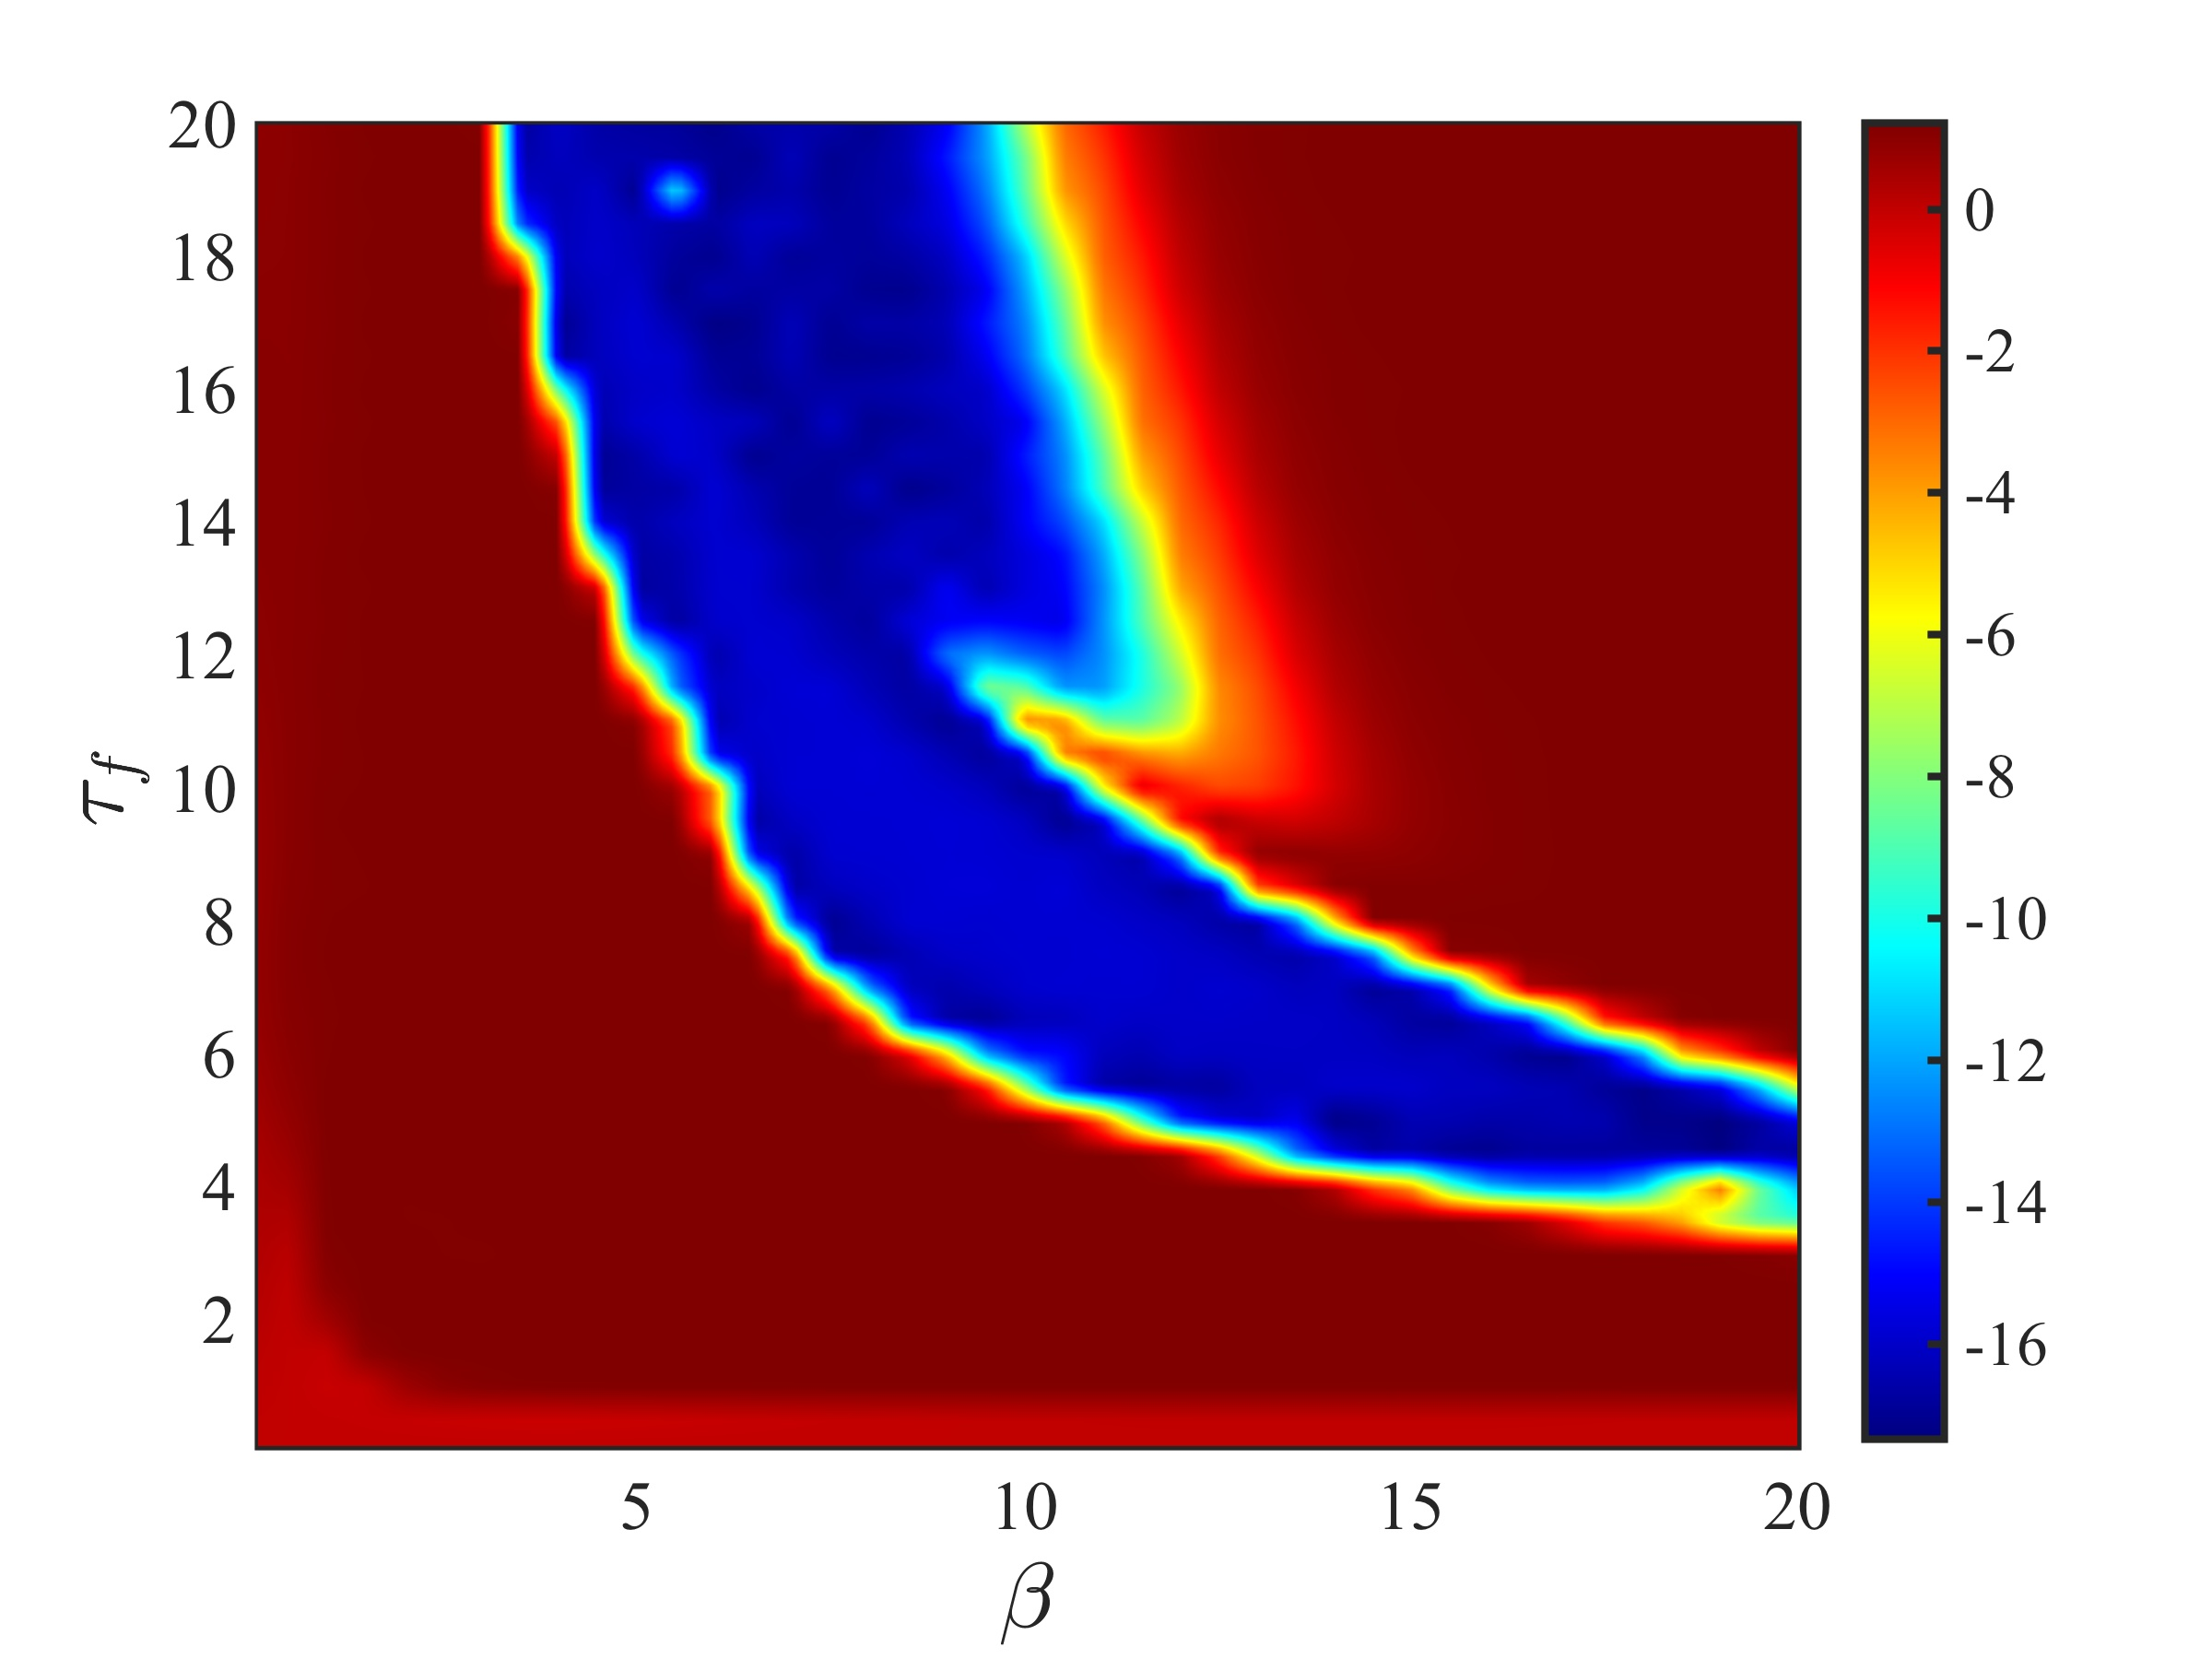
\includegraphics[width=\linewidth]{ACSkinnyQIn.jpg}
\caption{} 
\end{subfigure}
%\hspace*{\fill}
\hspace*{-0.5cm}
\begin{subfigure}{0.5\textwidth}
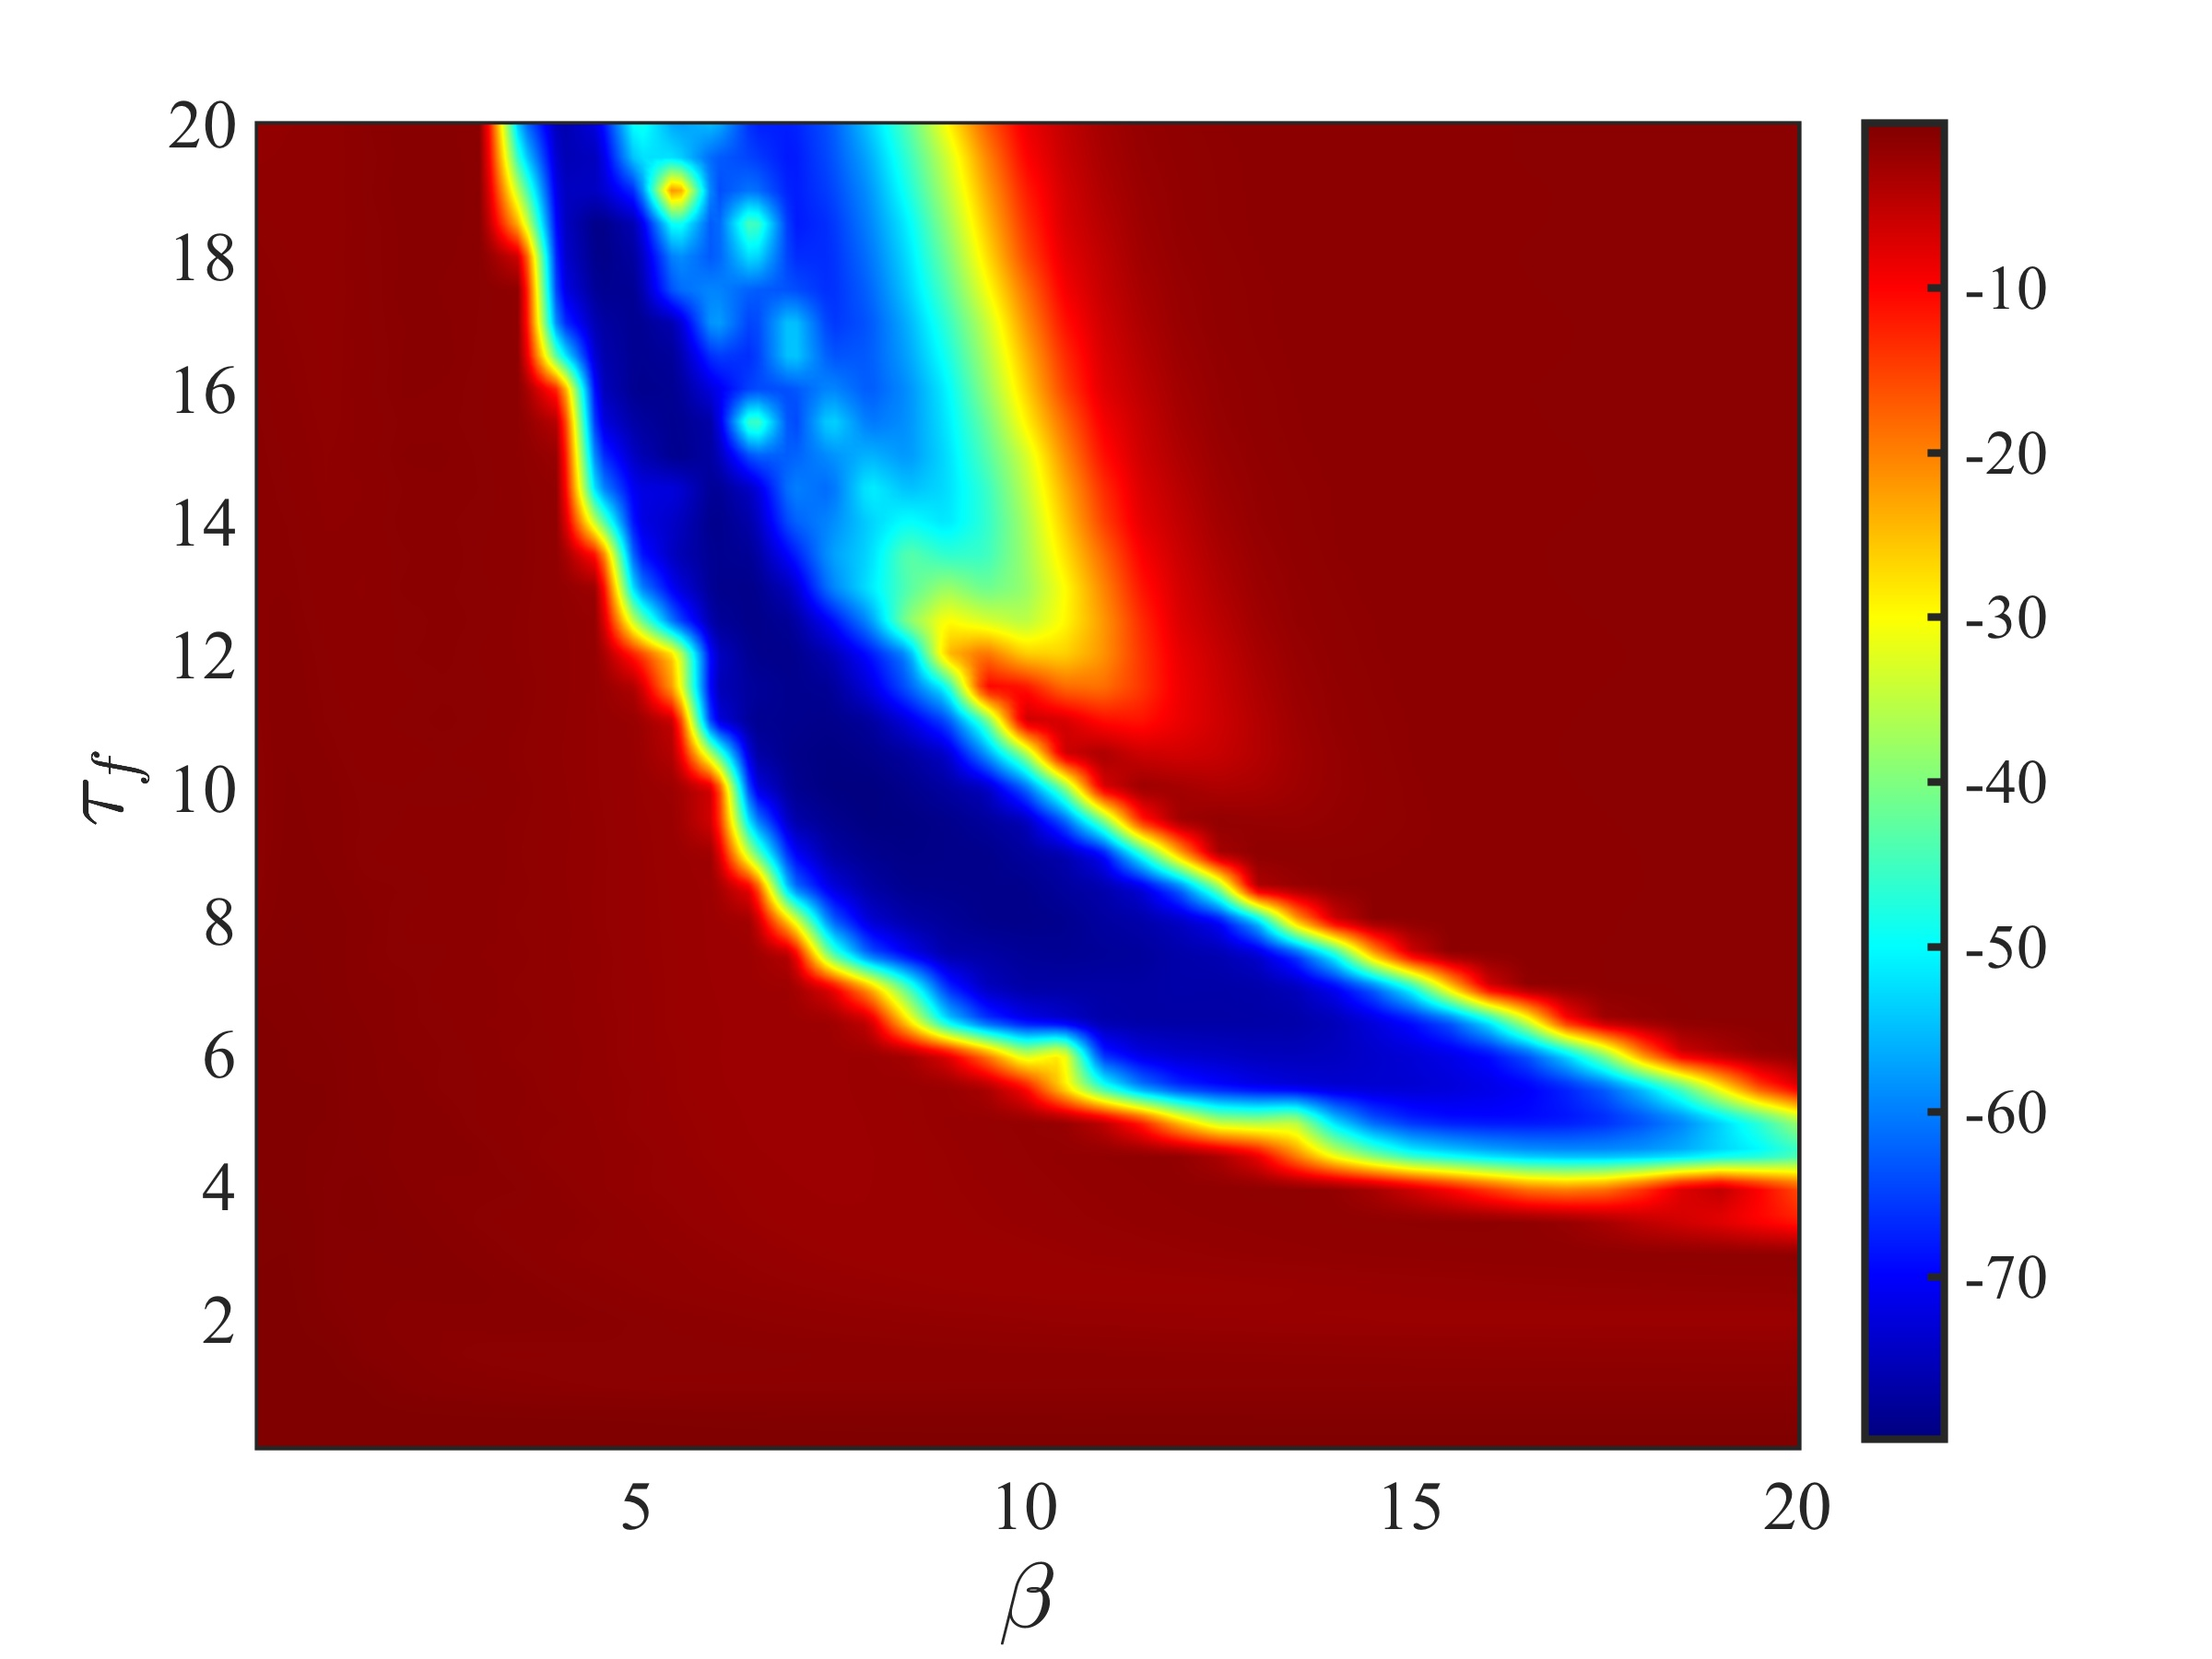
\includegraphics[width=\linewidth]{ACSkinnyQOut.jpg} 
\caption{} 
\end{subfigure} 
\centerline{
%\hspace{1cm}
\begin{subfigure}{\textwidth}
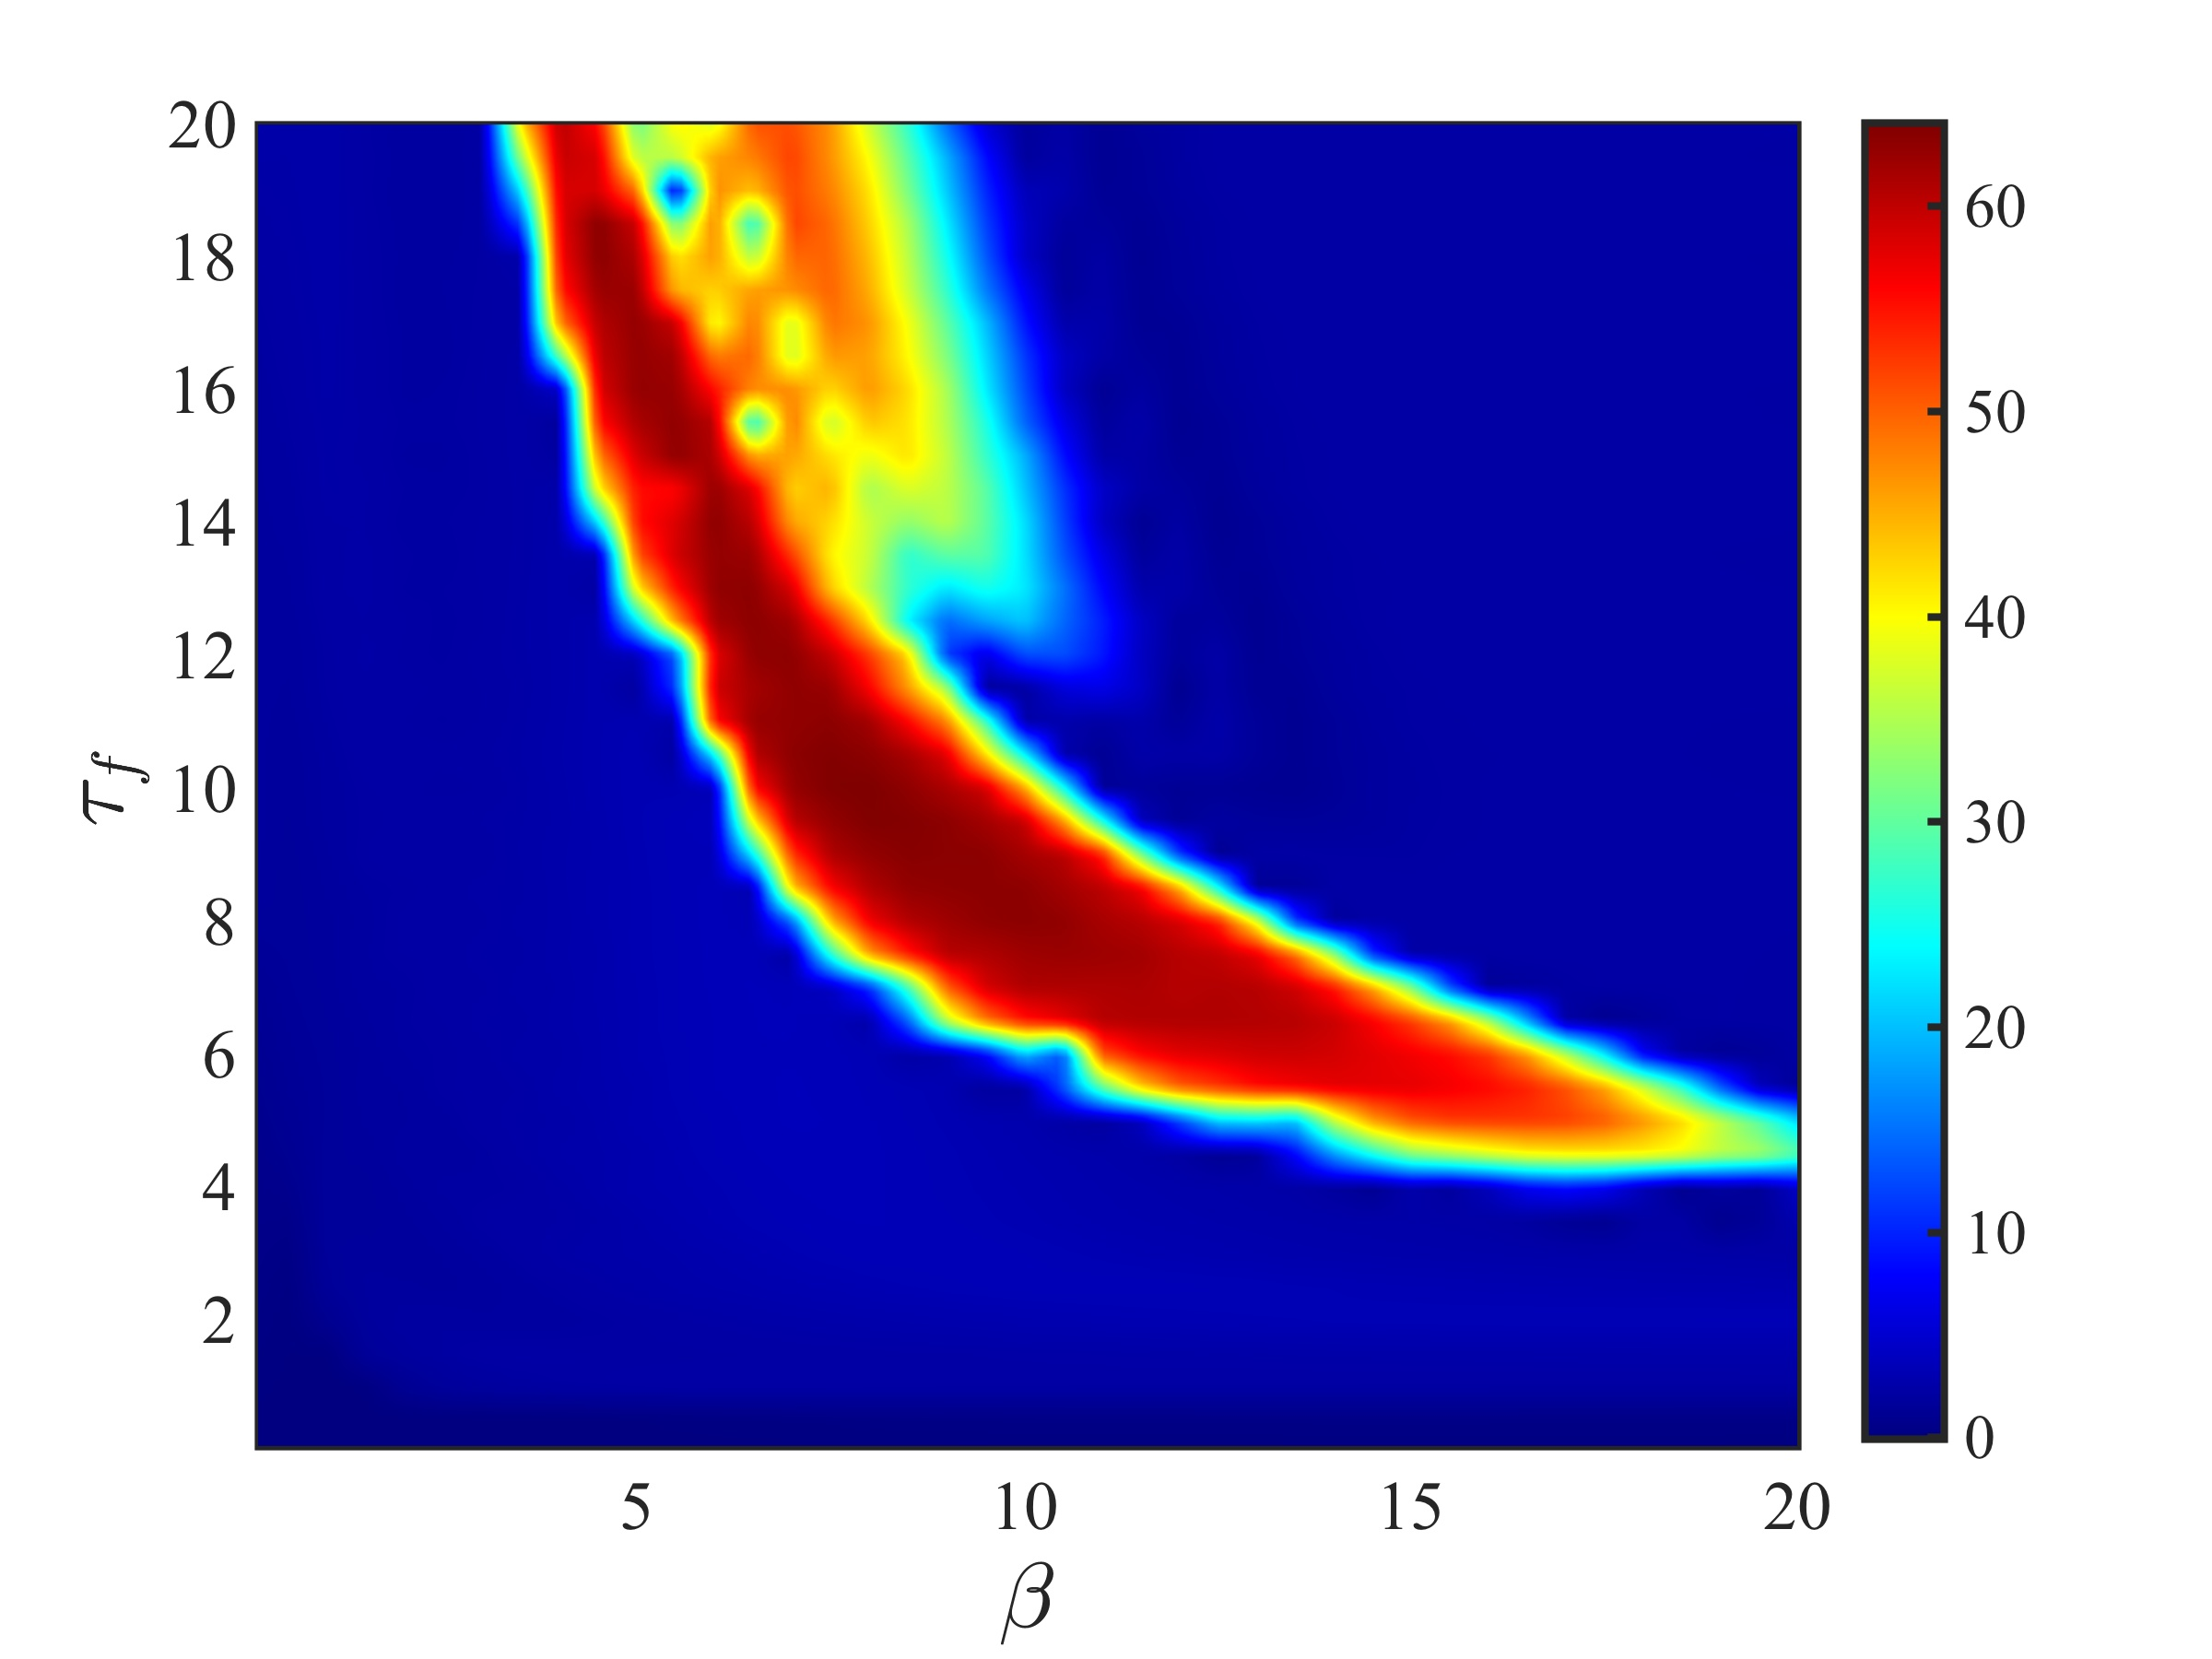
\includegraphics[width=\linewidth]{ACSkinnyQDiff.jpg} 
\caption{} 
\end{subfigure} }
  \rule{35em}{0.5pt}
\caption[Power Ratios Inside and Outside Tweezer with $\sigma_\phi = 0.5$ and $h_\phi = 2$]{
The density of the power ratios (a) inside and (b) outside of a narrow tweezer width $\sigma_\phi = 0.5$ and height $h_\phi = 2$.  The detuning for the system is $\Delta =  2.8074$ and each combination of parameter is evolved for $z_f = 10 = 4z^*$, with $z^* = 2.5$.  (a) The power ratio density inside the tweezer $Q_{\rm I}$, where blue ($Q_{\rm I}=0$) is complete power inside the tweezer at $z_f$ and red ($Q_{\rm I}=1$) is no power inside the tweezer at $z_f$.  (b) The power ratio density outside the tweezer $Q_{\rm O}$, where $Q_{\rm O}$ = 0 depicts no change in power.  (c) The difference in power ratios inside and outside the tweezer, $Q_{\rm I} - Q_{\rm O}$.  The difference between the power ratios (c) defines the thresholds for tweezed CSs for all blue regions, no-CSs for all green regions, and non-tweezed CSs for all red regions.  
}
\label{fig:ACSkinnyQ}
\end{figure}

Figure~\ref{fig:ACRegularQ} depicts the density of the power ratios inside $Q_{\rm I}$ (top) and outside $Q_{\rm O}$ (bottom) of a tweezer with width $\sigma_\phi = 1$ and $h_\phi = 2$.  For the full LL Eq.~(\ref{eq:LLETweeze}) with $u_{\rm in} = 2$, the steady state CS is found centered at $\tau_0 = 0$ using a Newton-Krylov solver and the power-balance constraint Eq.~(\ref{LLConstraint}) which selects a particular detuning parameter $\Delta =  3.1488$ for the system.  
\begin{figure}[htb!]
\centering
\hspace{0cm}
\begin{subfigure}{0.5\textwidth}
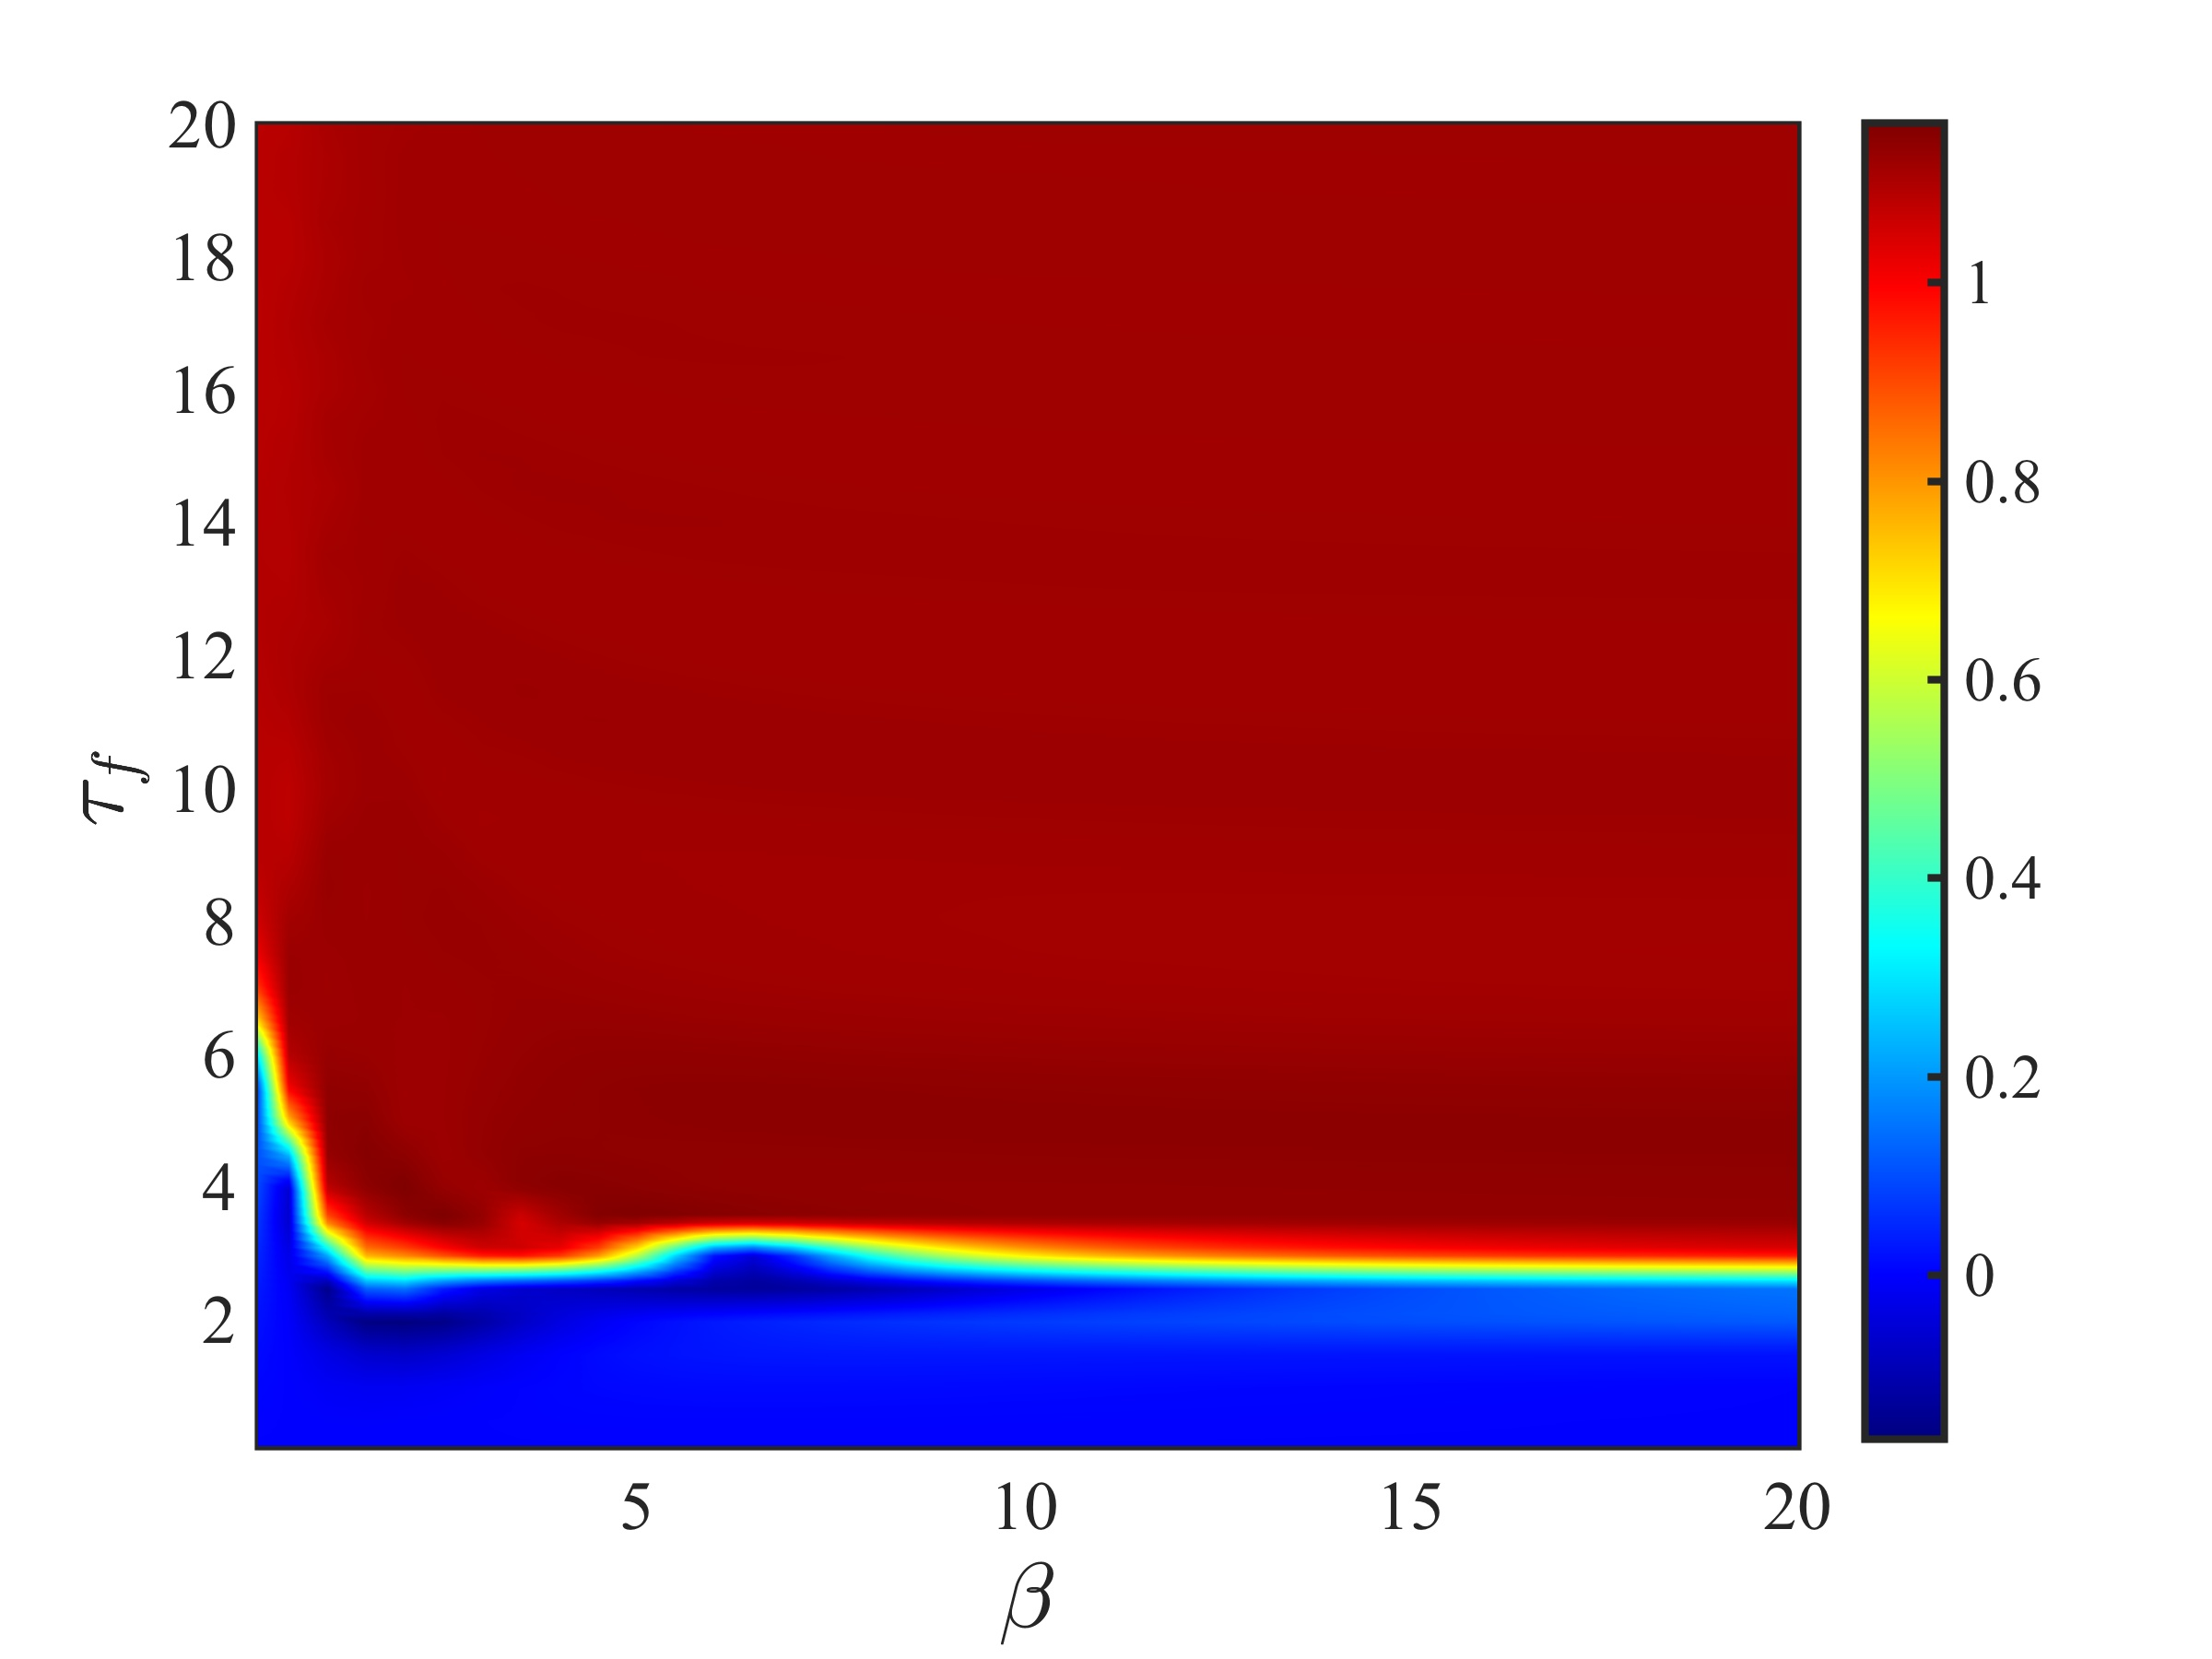
\includegraphics[width=\linewidth]{ACRegularQIn.jpg}
\caption{} 
\end{subfigure}
%\hspace*{\fill}
\hspace*{-0.5cm}
\begin{subfigure}{0.5\textwidth}
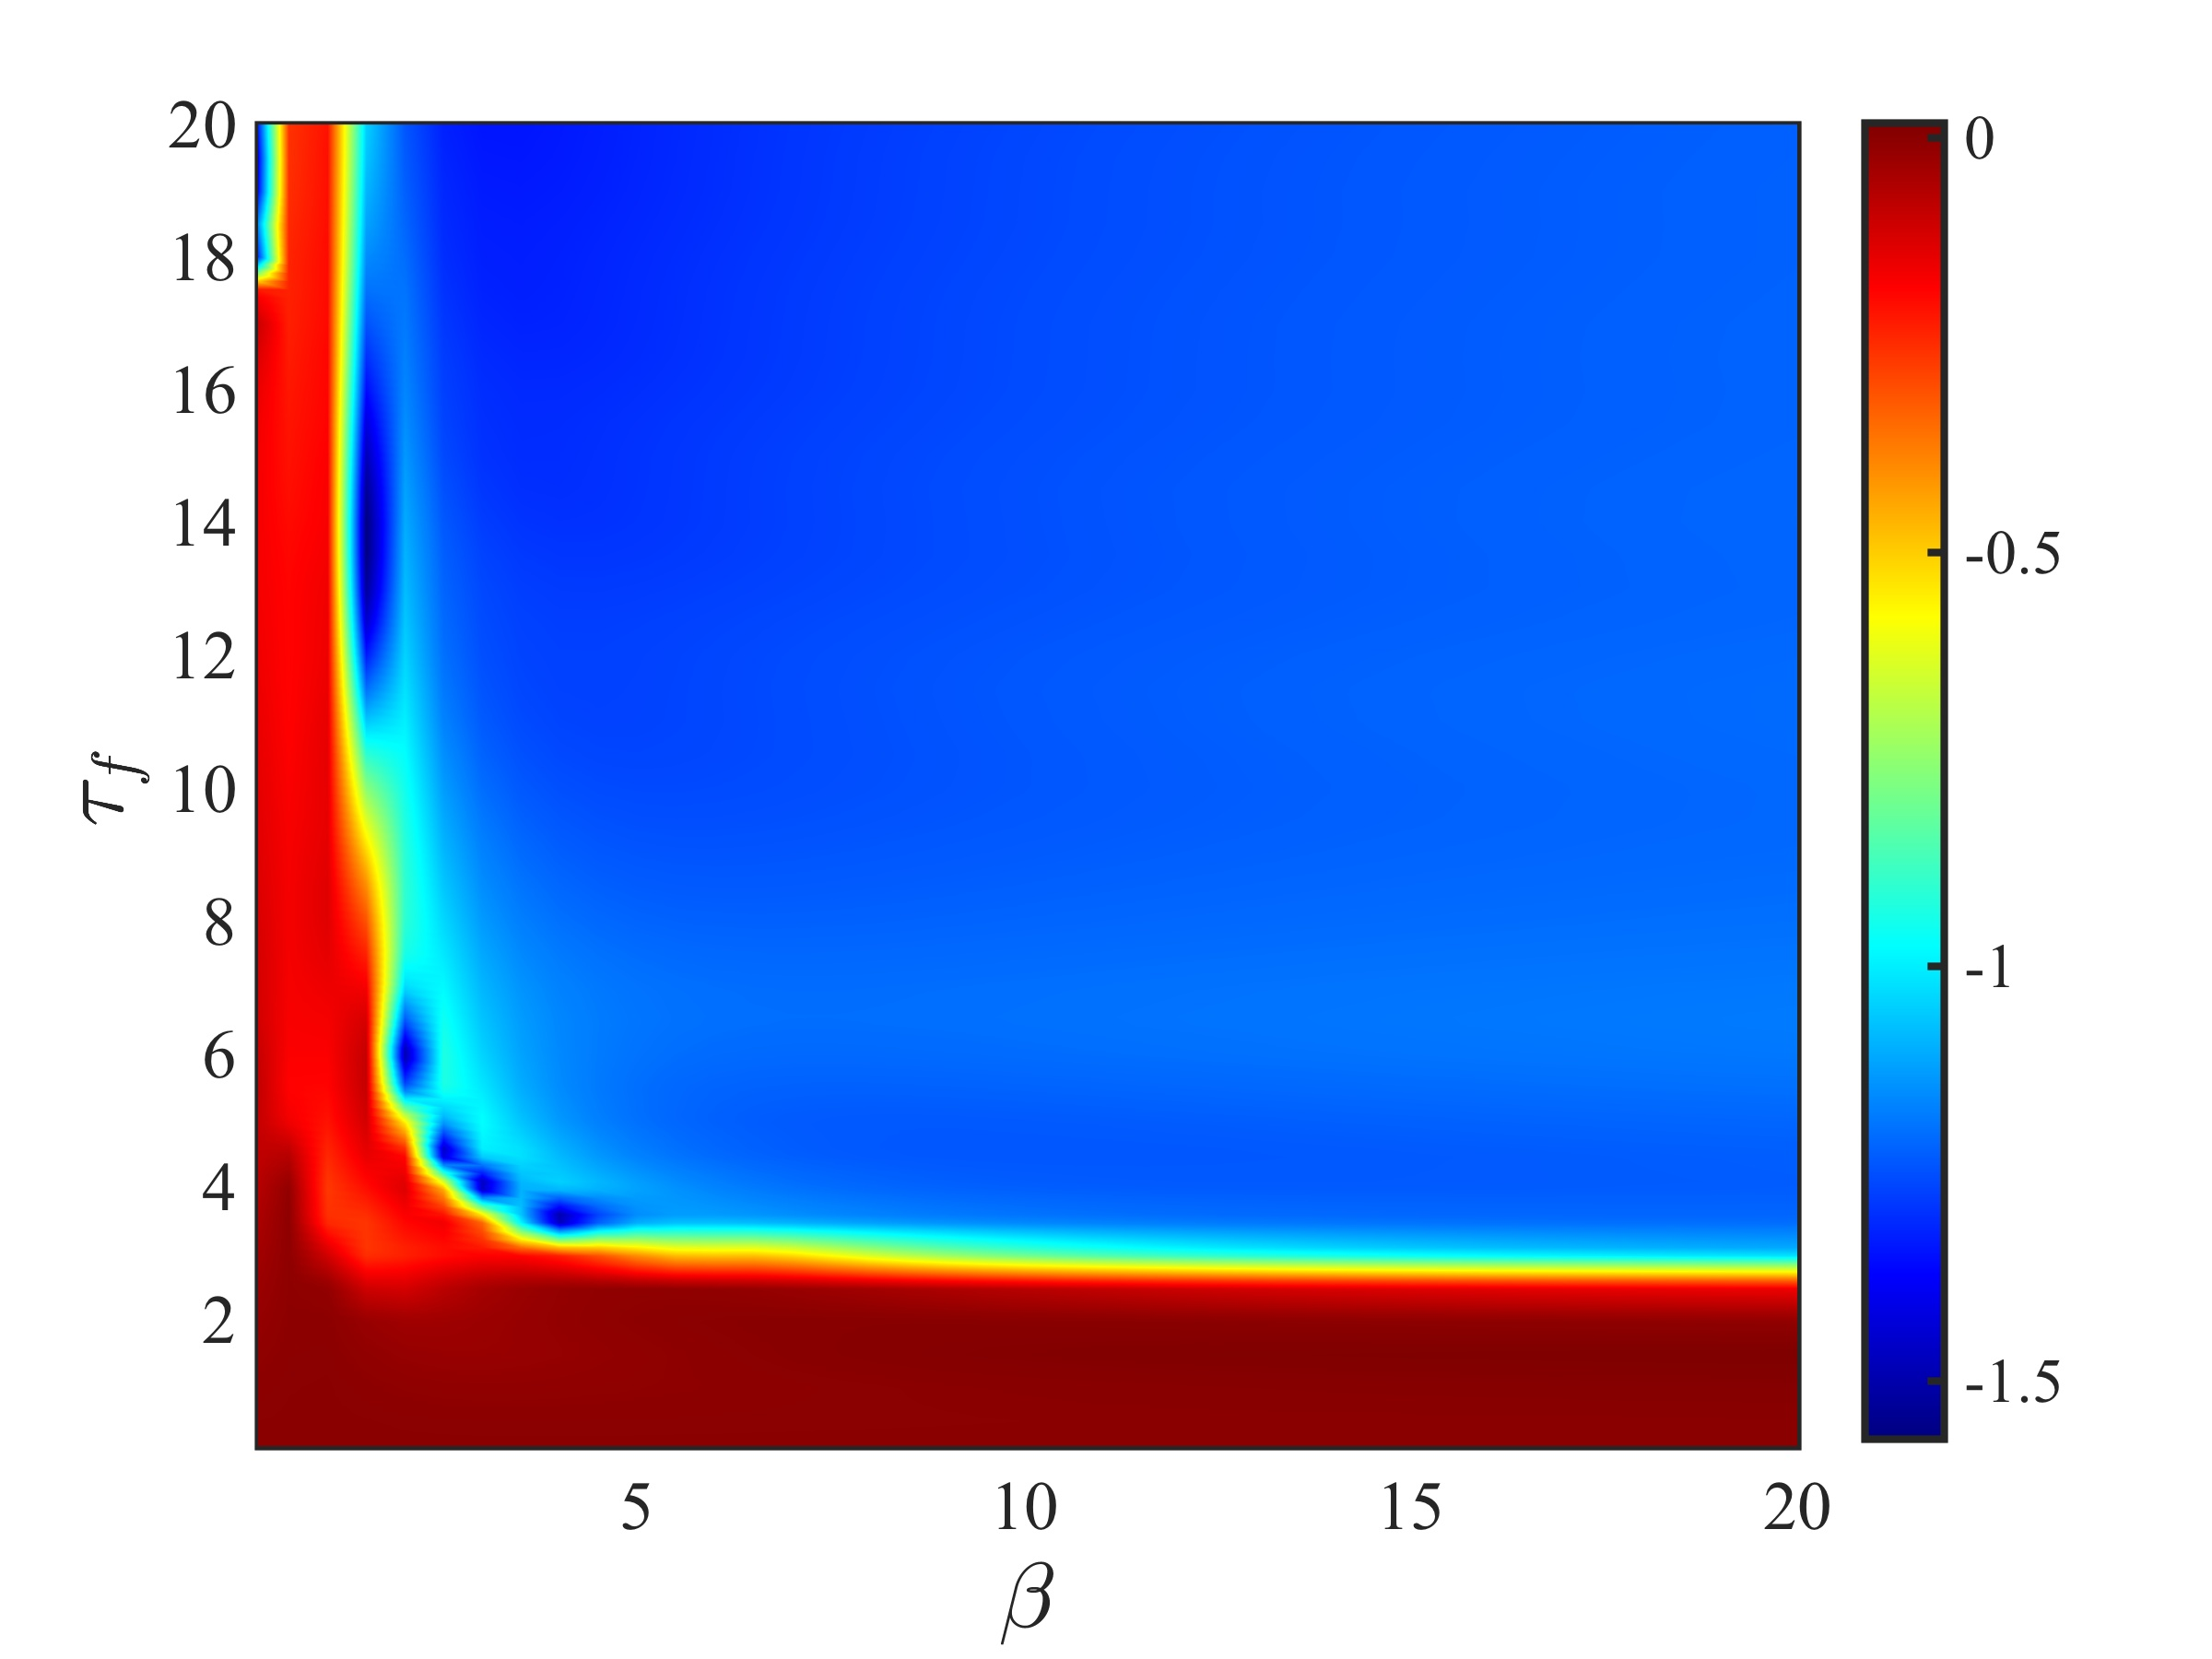
\includegraphics[width=\linewidth]{ACRegularQOut.jpg} 
\caption{} 
\end{subfigure} 
\centerline{
%\hspace{1cm}
\begin{subfigure}{\textwidth}
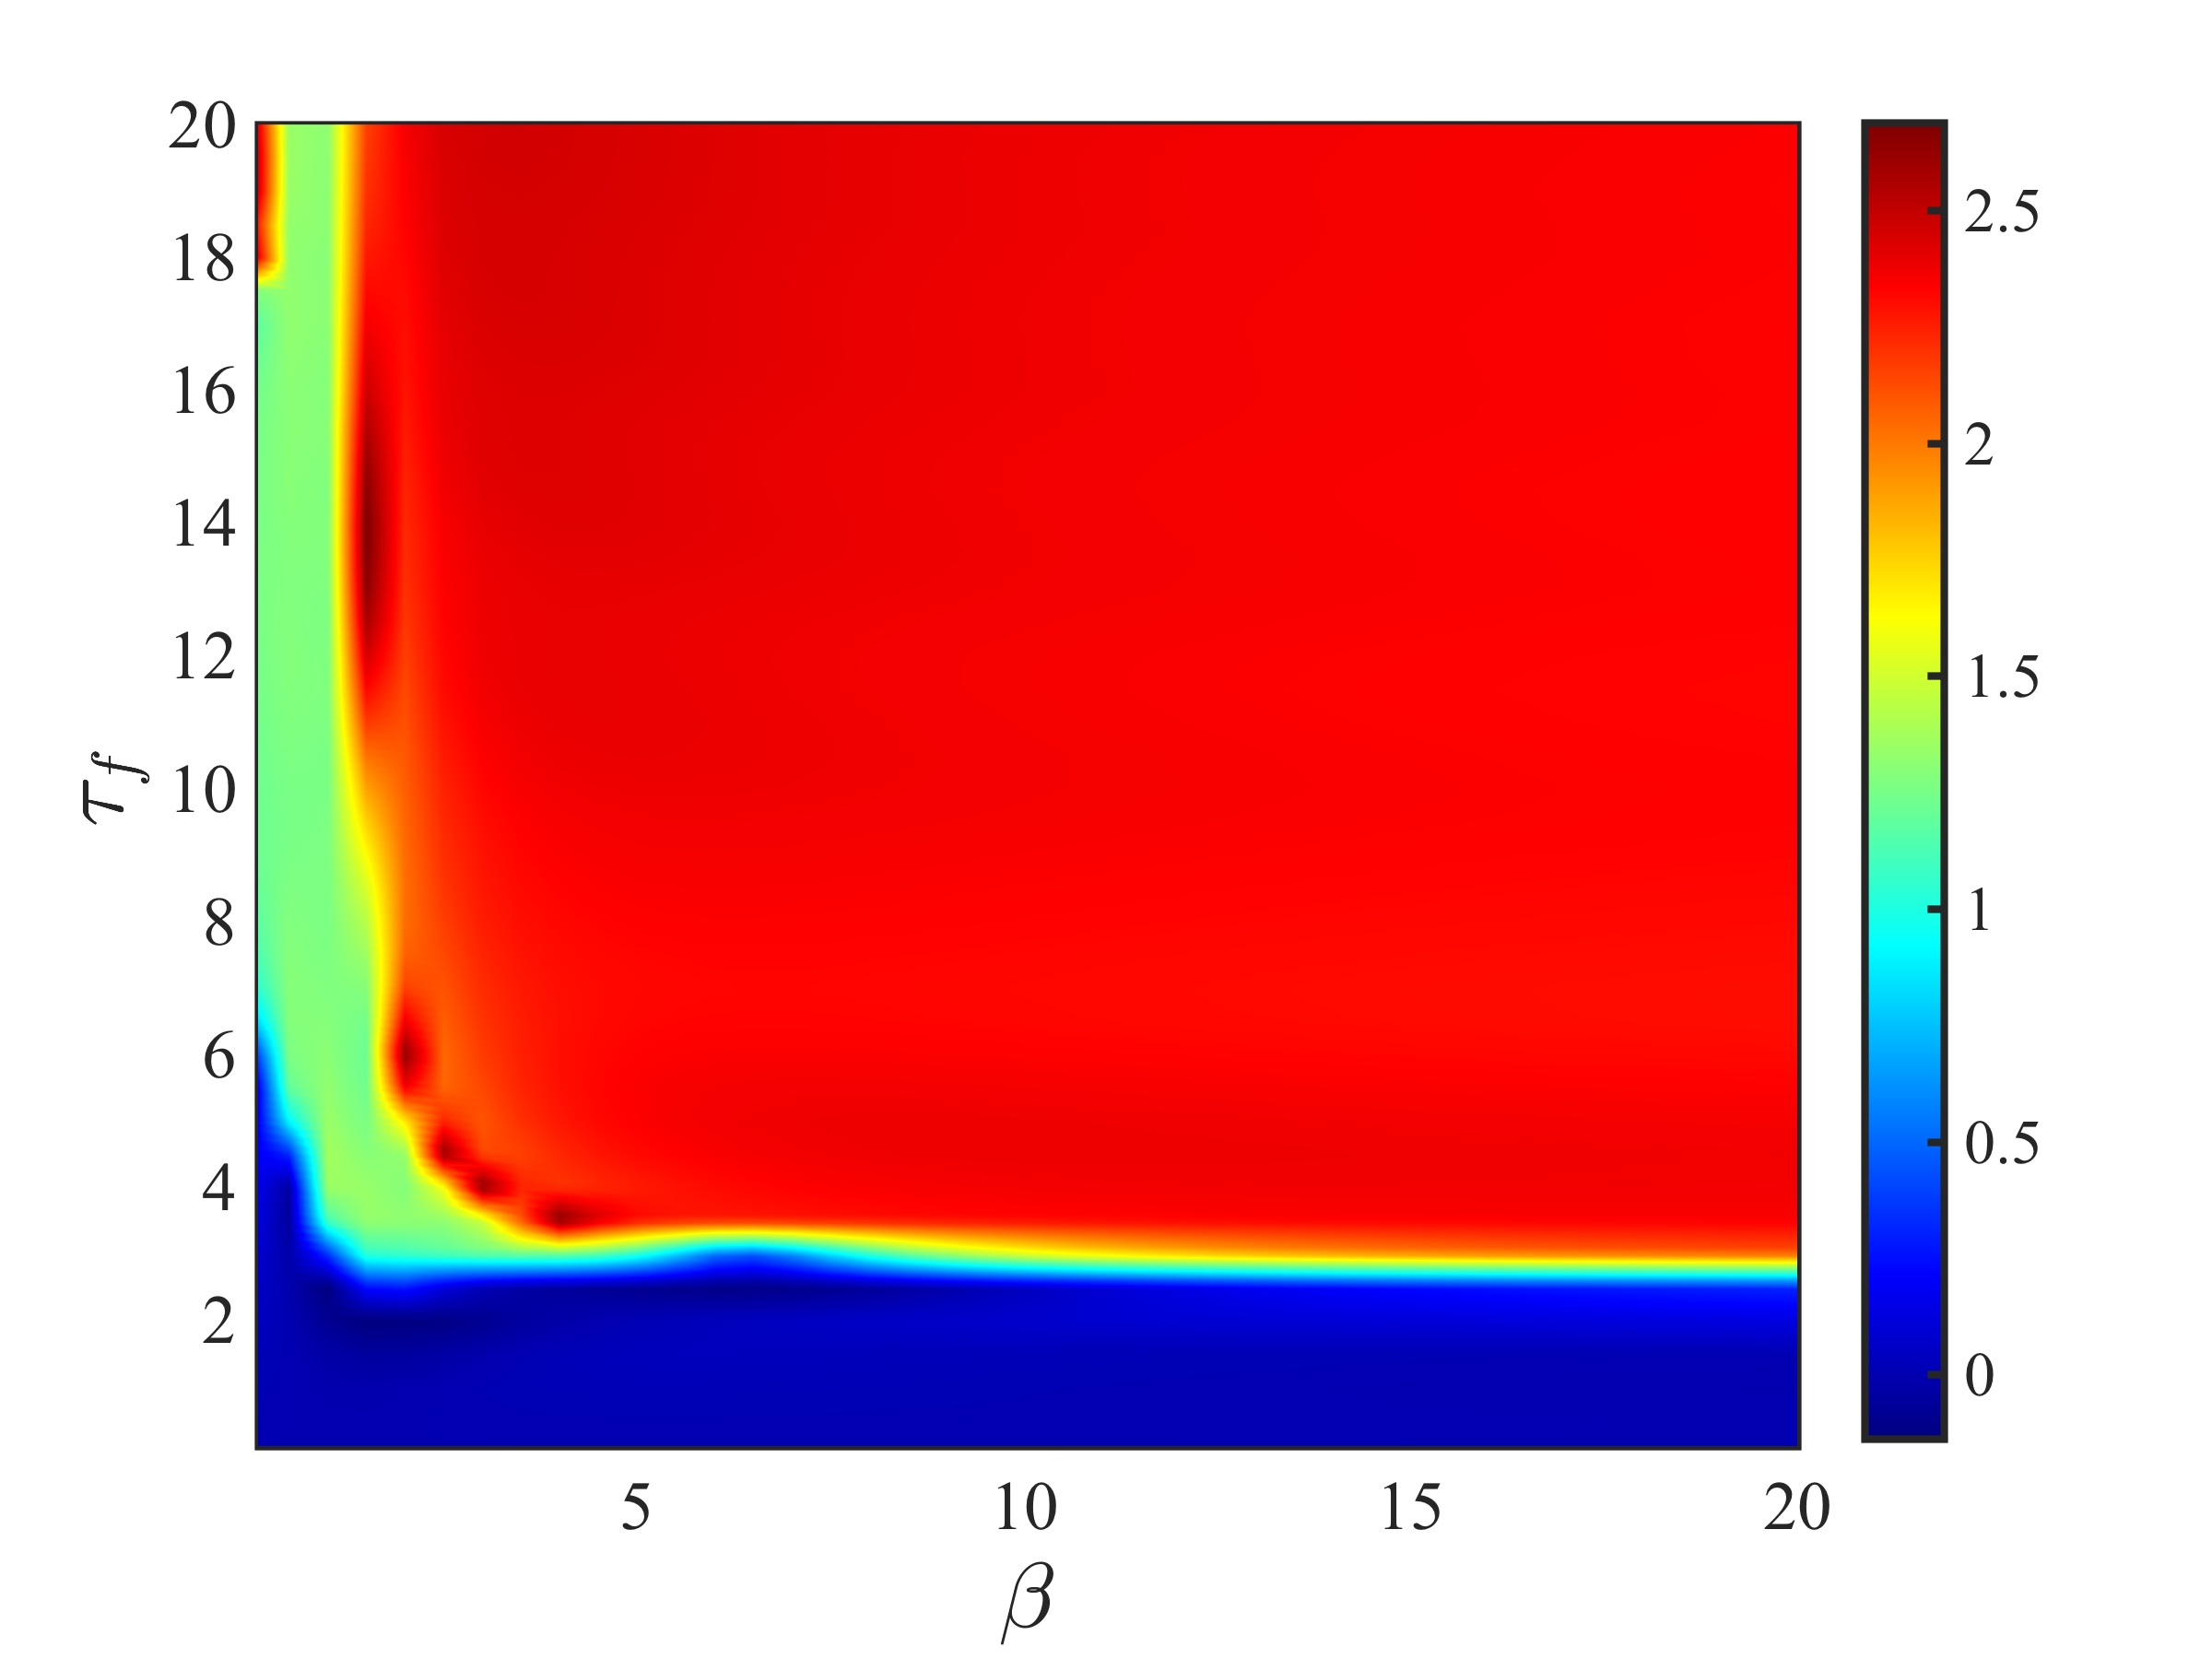
\includegraphics[width=\linewidth]{ACRegularQDiff.jpg} 
\caption{} 
\end{subfigure} }
  \rule{35em}{0.5pt}
\caption[Power Ratios Inside and Outside Tweezer with $\sigma_\phi = 1$ and $h_\phi = 2$]{
Power ratios as in Fig.~\ref{fig:ACSkinnyQ} but for a  tweezer with width $\sigma_\phi = 1$ and height $h_\phi = 2$.  The detuning for the system is $\Delta =  3.1488$.   Same layout as in Fig.~\ref{fig:ACSkinnyQ}.  The difference power ratio (c) defines the thresholds for tweezed CSs for all blue regions, no-CSs for all green regions, and non-tweezed CSs for all red regions.  
}
\label{fig:ACRegularQ}
\end{figure}

Figure~\ref{fig:ACFatQ} depicts the density of the power ratios inside $Q_{\rm I}$ (top) and outside $Q_{\rm O}$ (bottom) of a tweezer with width $\sigma_\phi = 2$ and $h_\phi = 2$.  For the full LL Eq.~(\ref{eq:LLETweeze}) with $u_{\rm in} = 2$, the steady state CS is found centered at $\tau_0 = 0$ using a Newton-Krylov solver and the power-balance constraint Eq.~(\ref{LLConstraint}) which selects a detuning parameter $\Delta =  3.3830$ for the system.  The power ratio difference $Q_{\rm diff}$ defines the threshold between the existence of tweezed CSs and no-CSs for most $\beta$ at approximately $\tau_f = 4$.

\begin{figure}[htb!]
\centering
\hspace{0cm}
\begin{subfigure}{0.5\textwidth}
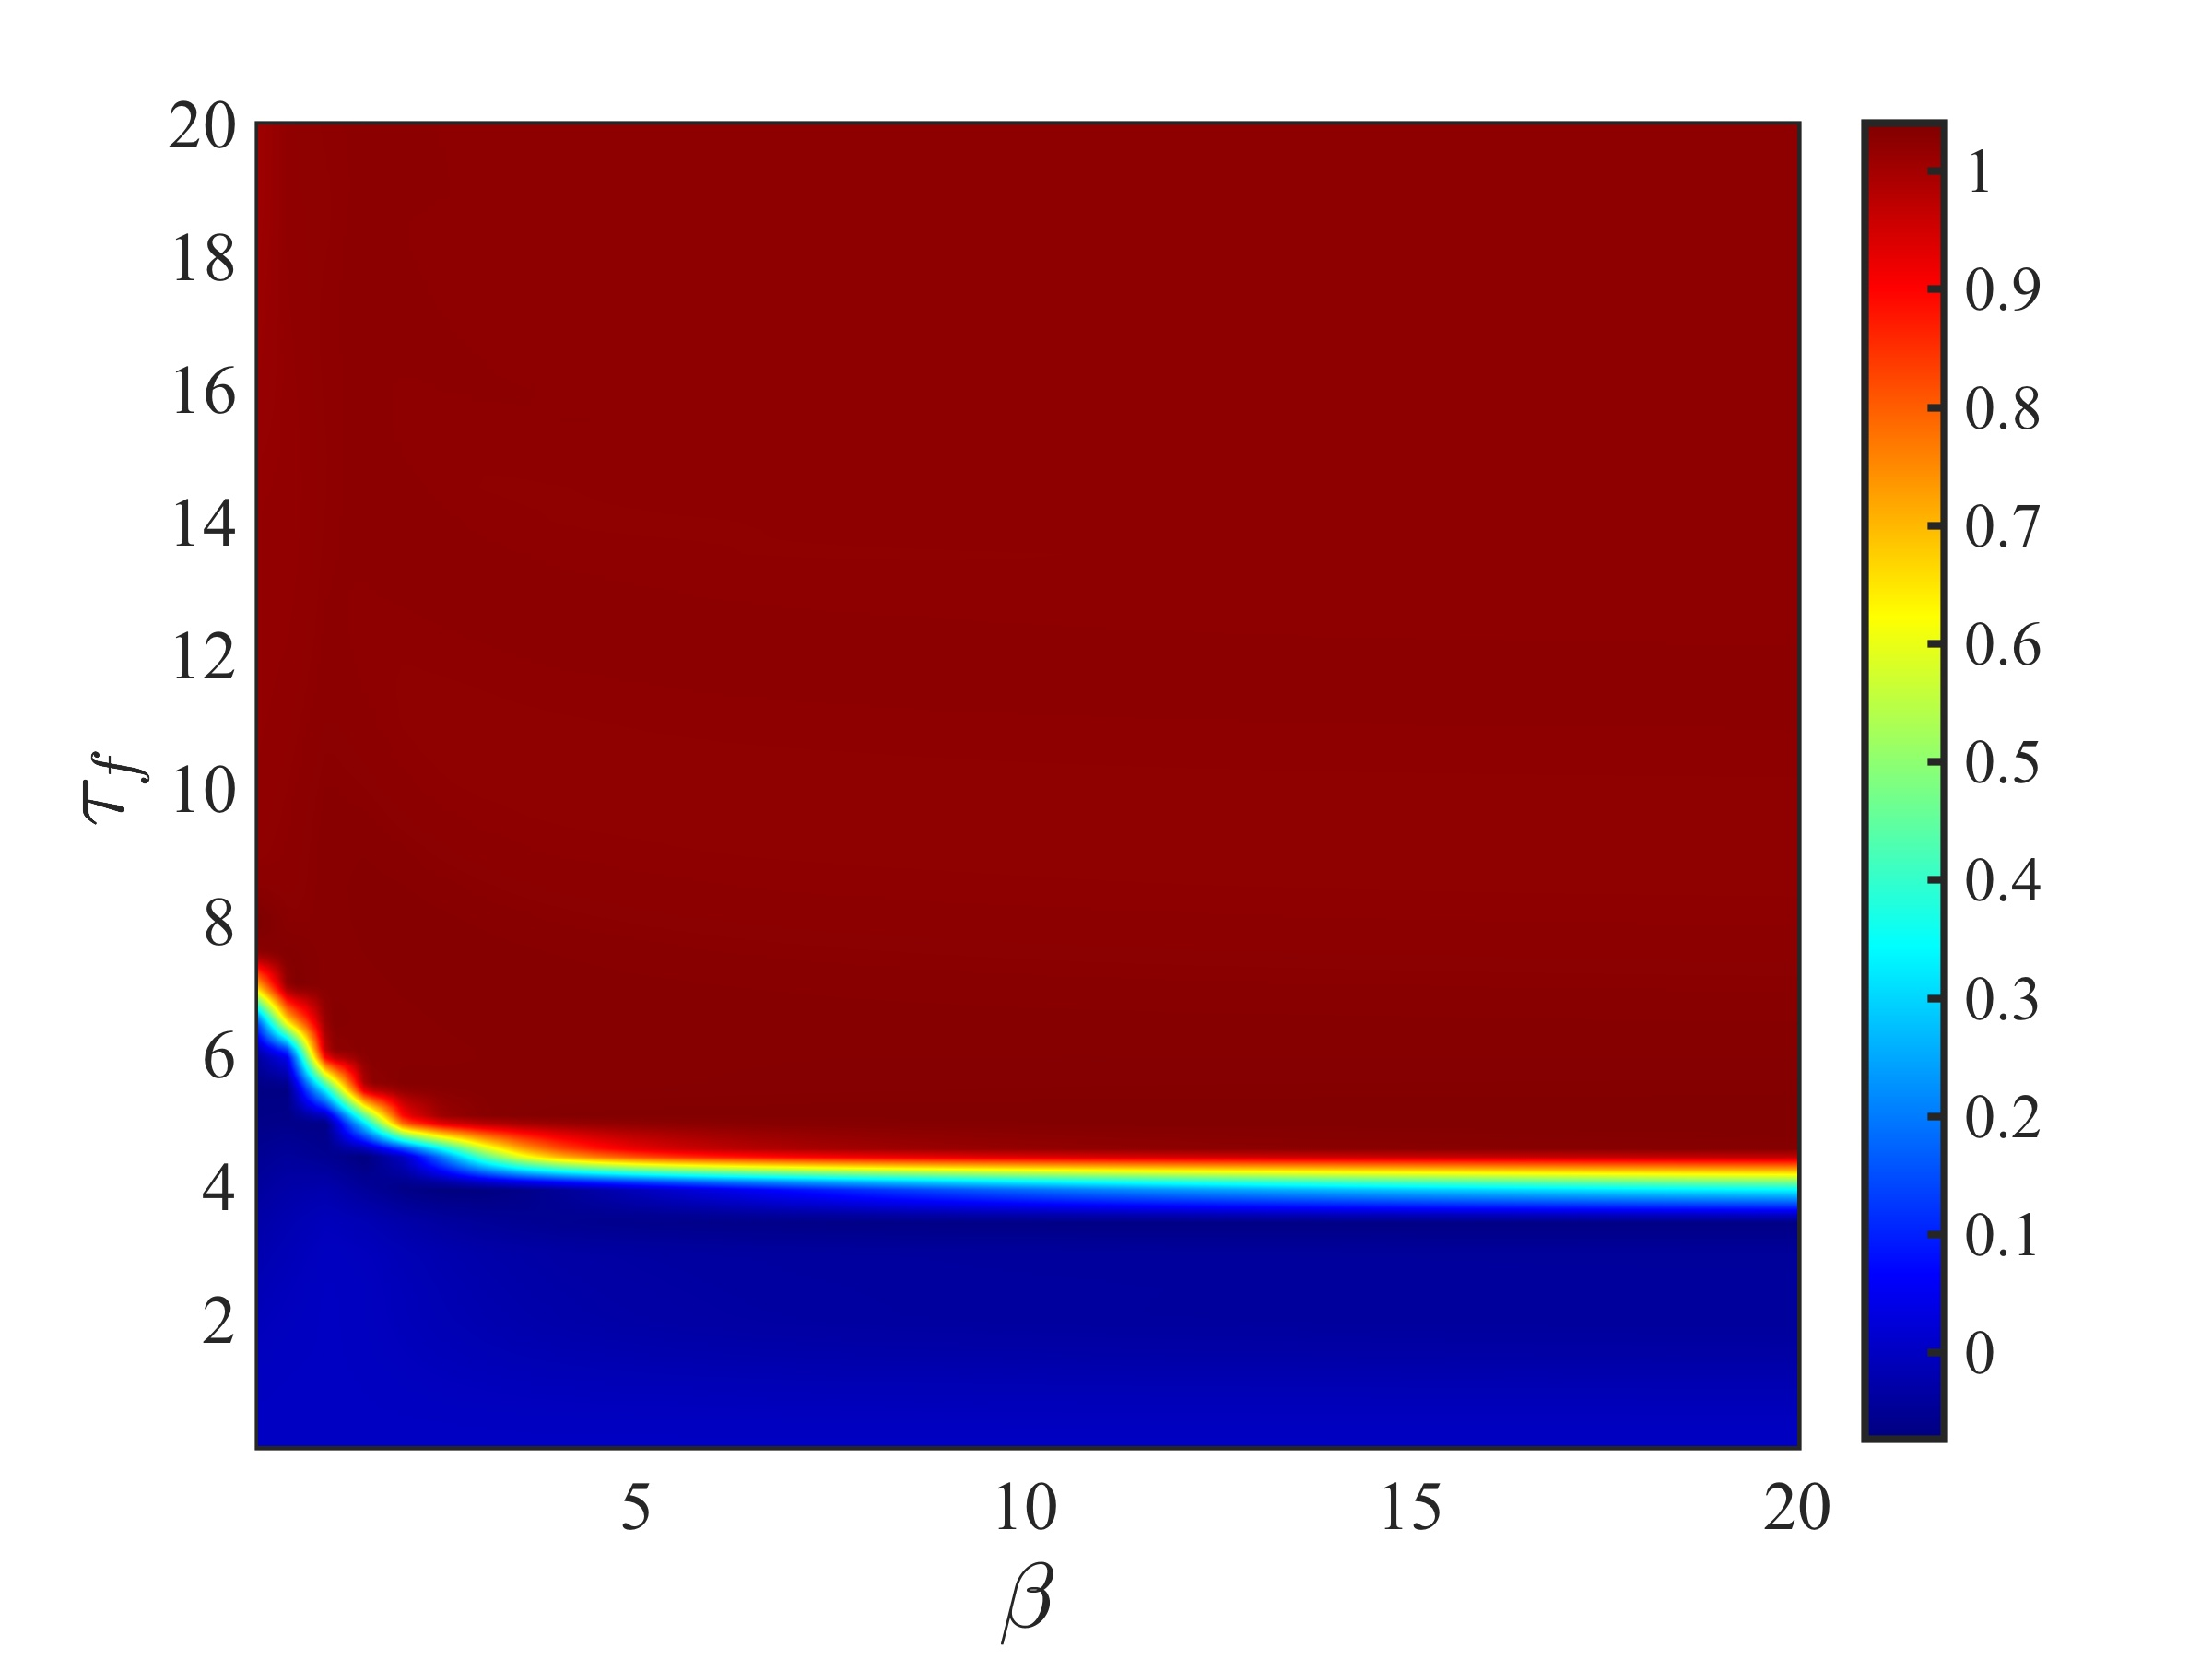
\includegraphics[width=\linewidth]{ACFatQIn.jpg}
\caption{} 
\end{subfigure}
%\hspace*{\fill}
\hspace*{-0.5cm}
\begin{subfigure}{0.5\textwidth}
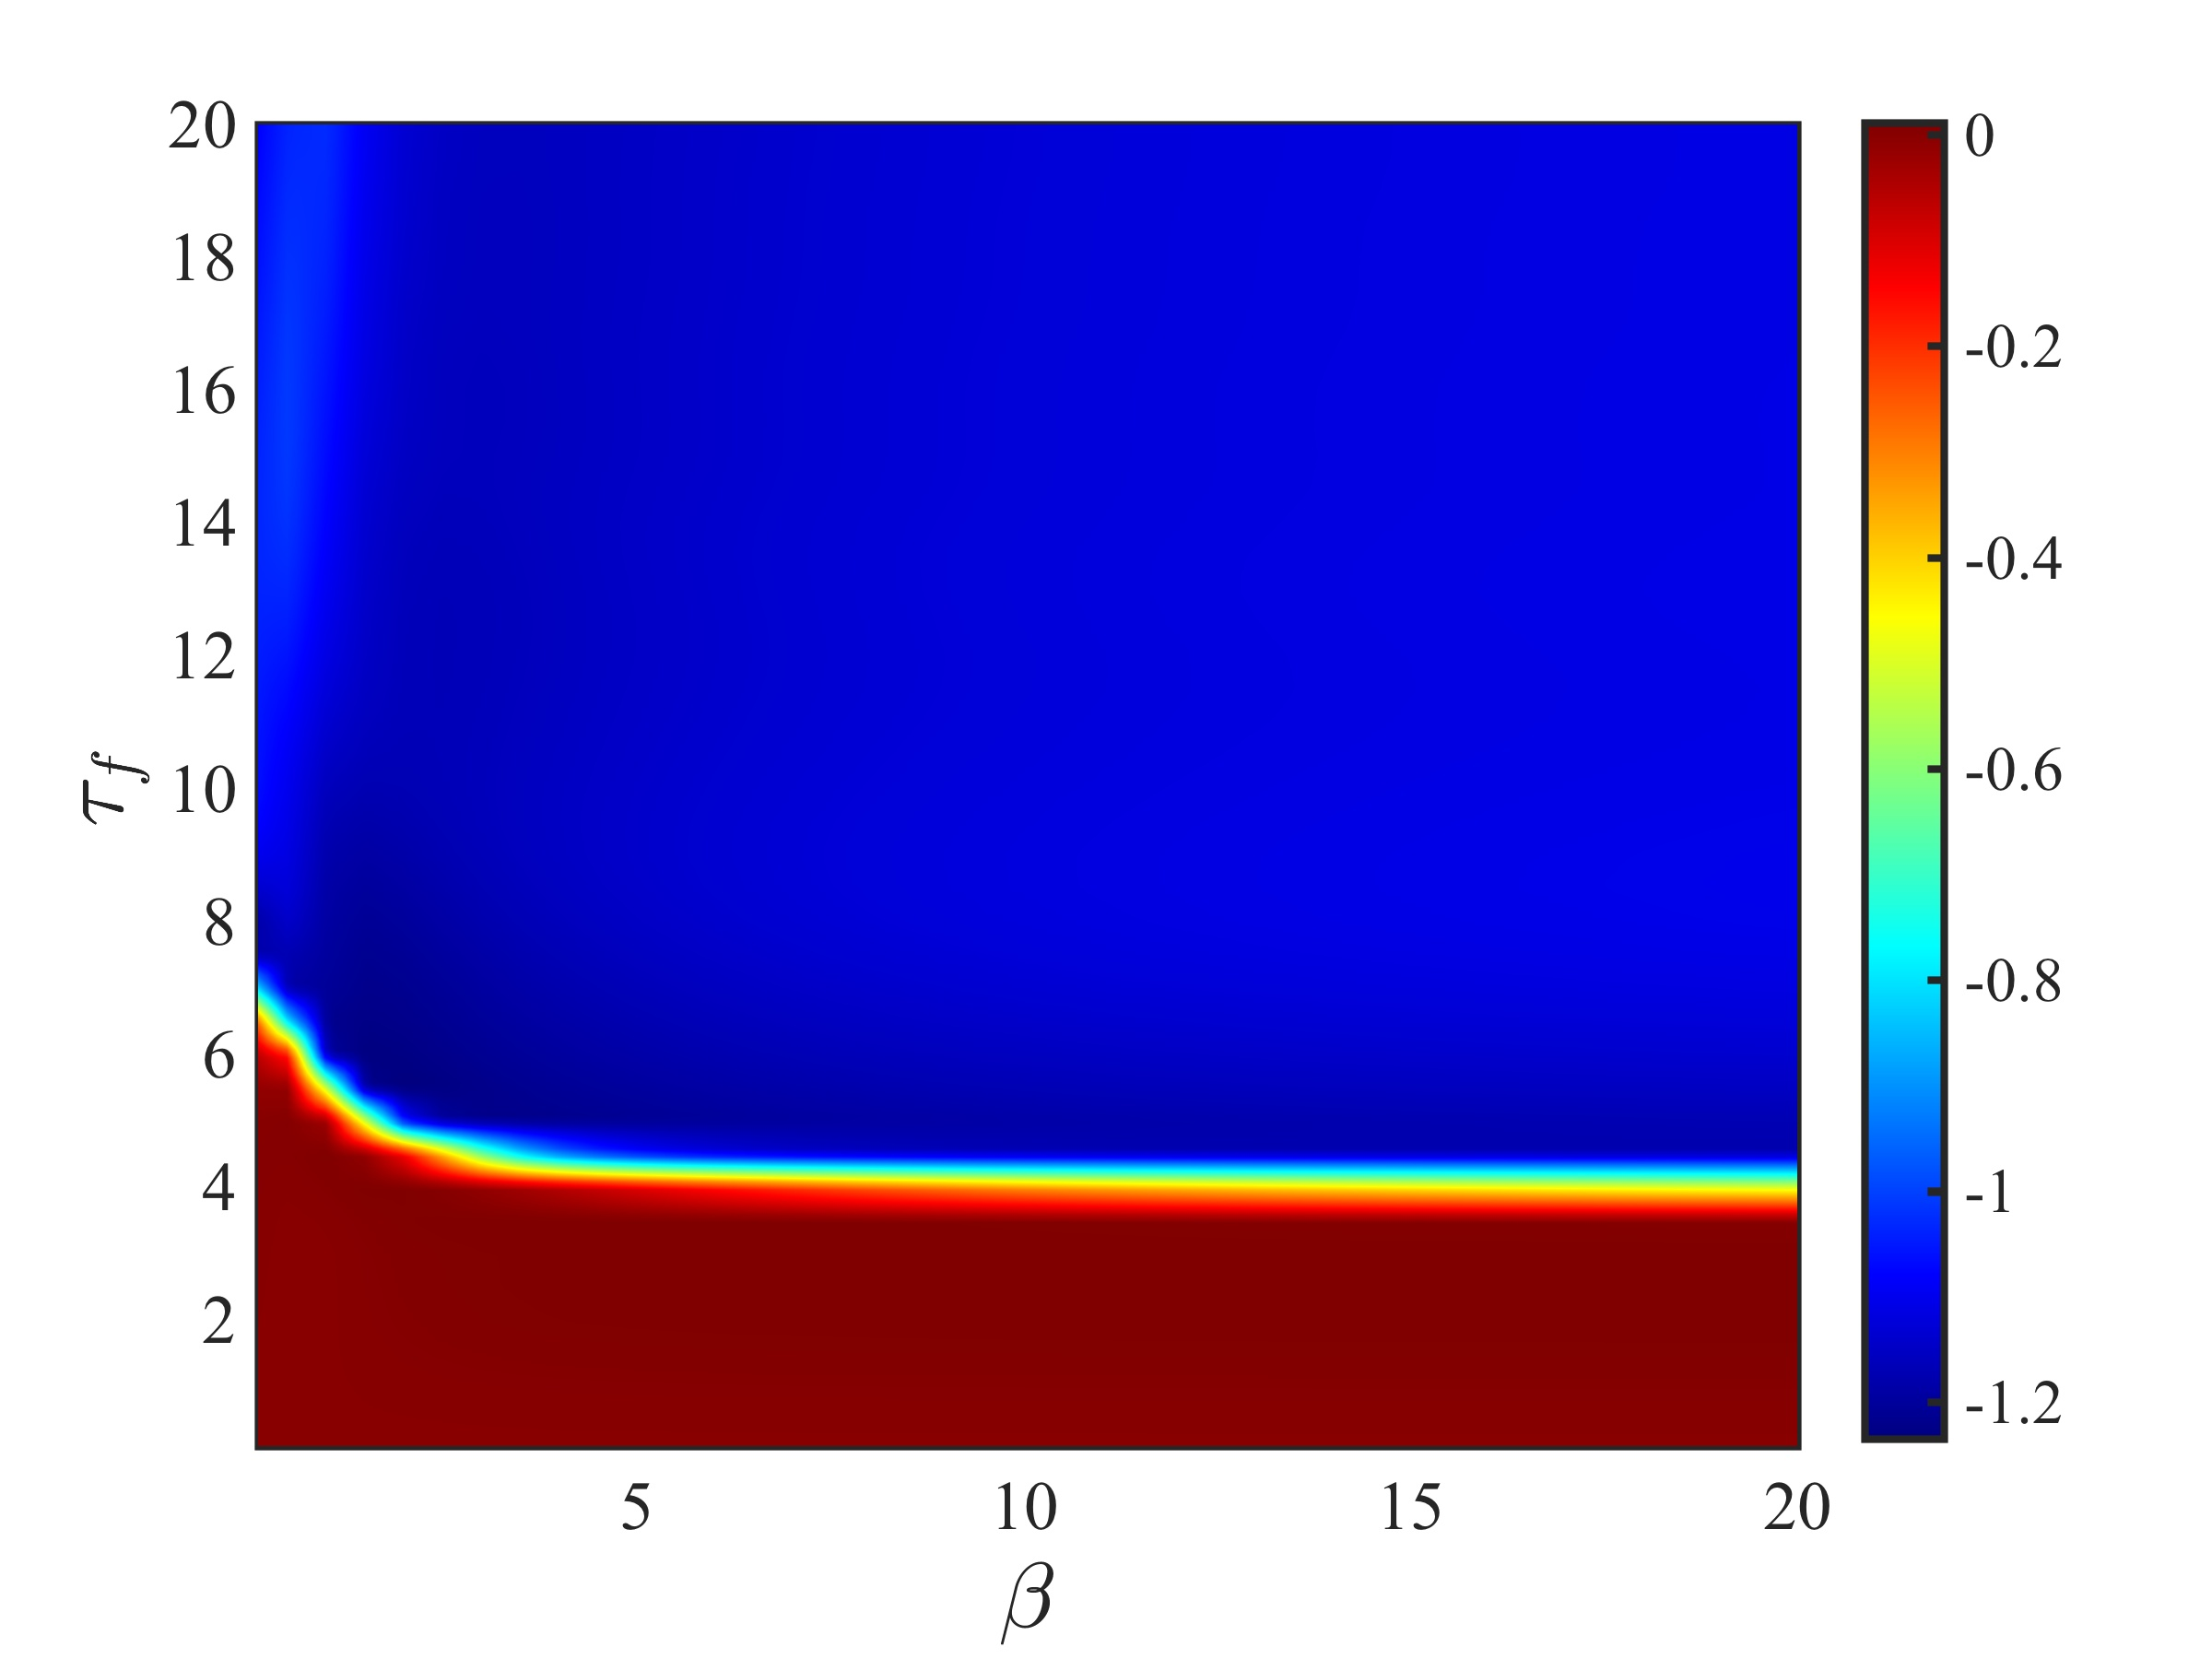
\includegraphics[width=\linewidth]{ACFatQOut.jpg} 
\caption{} 
\end{subfigure} 
\centerline{
%\hspace{1cm}
\begin{subfigure}{\textwidth}
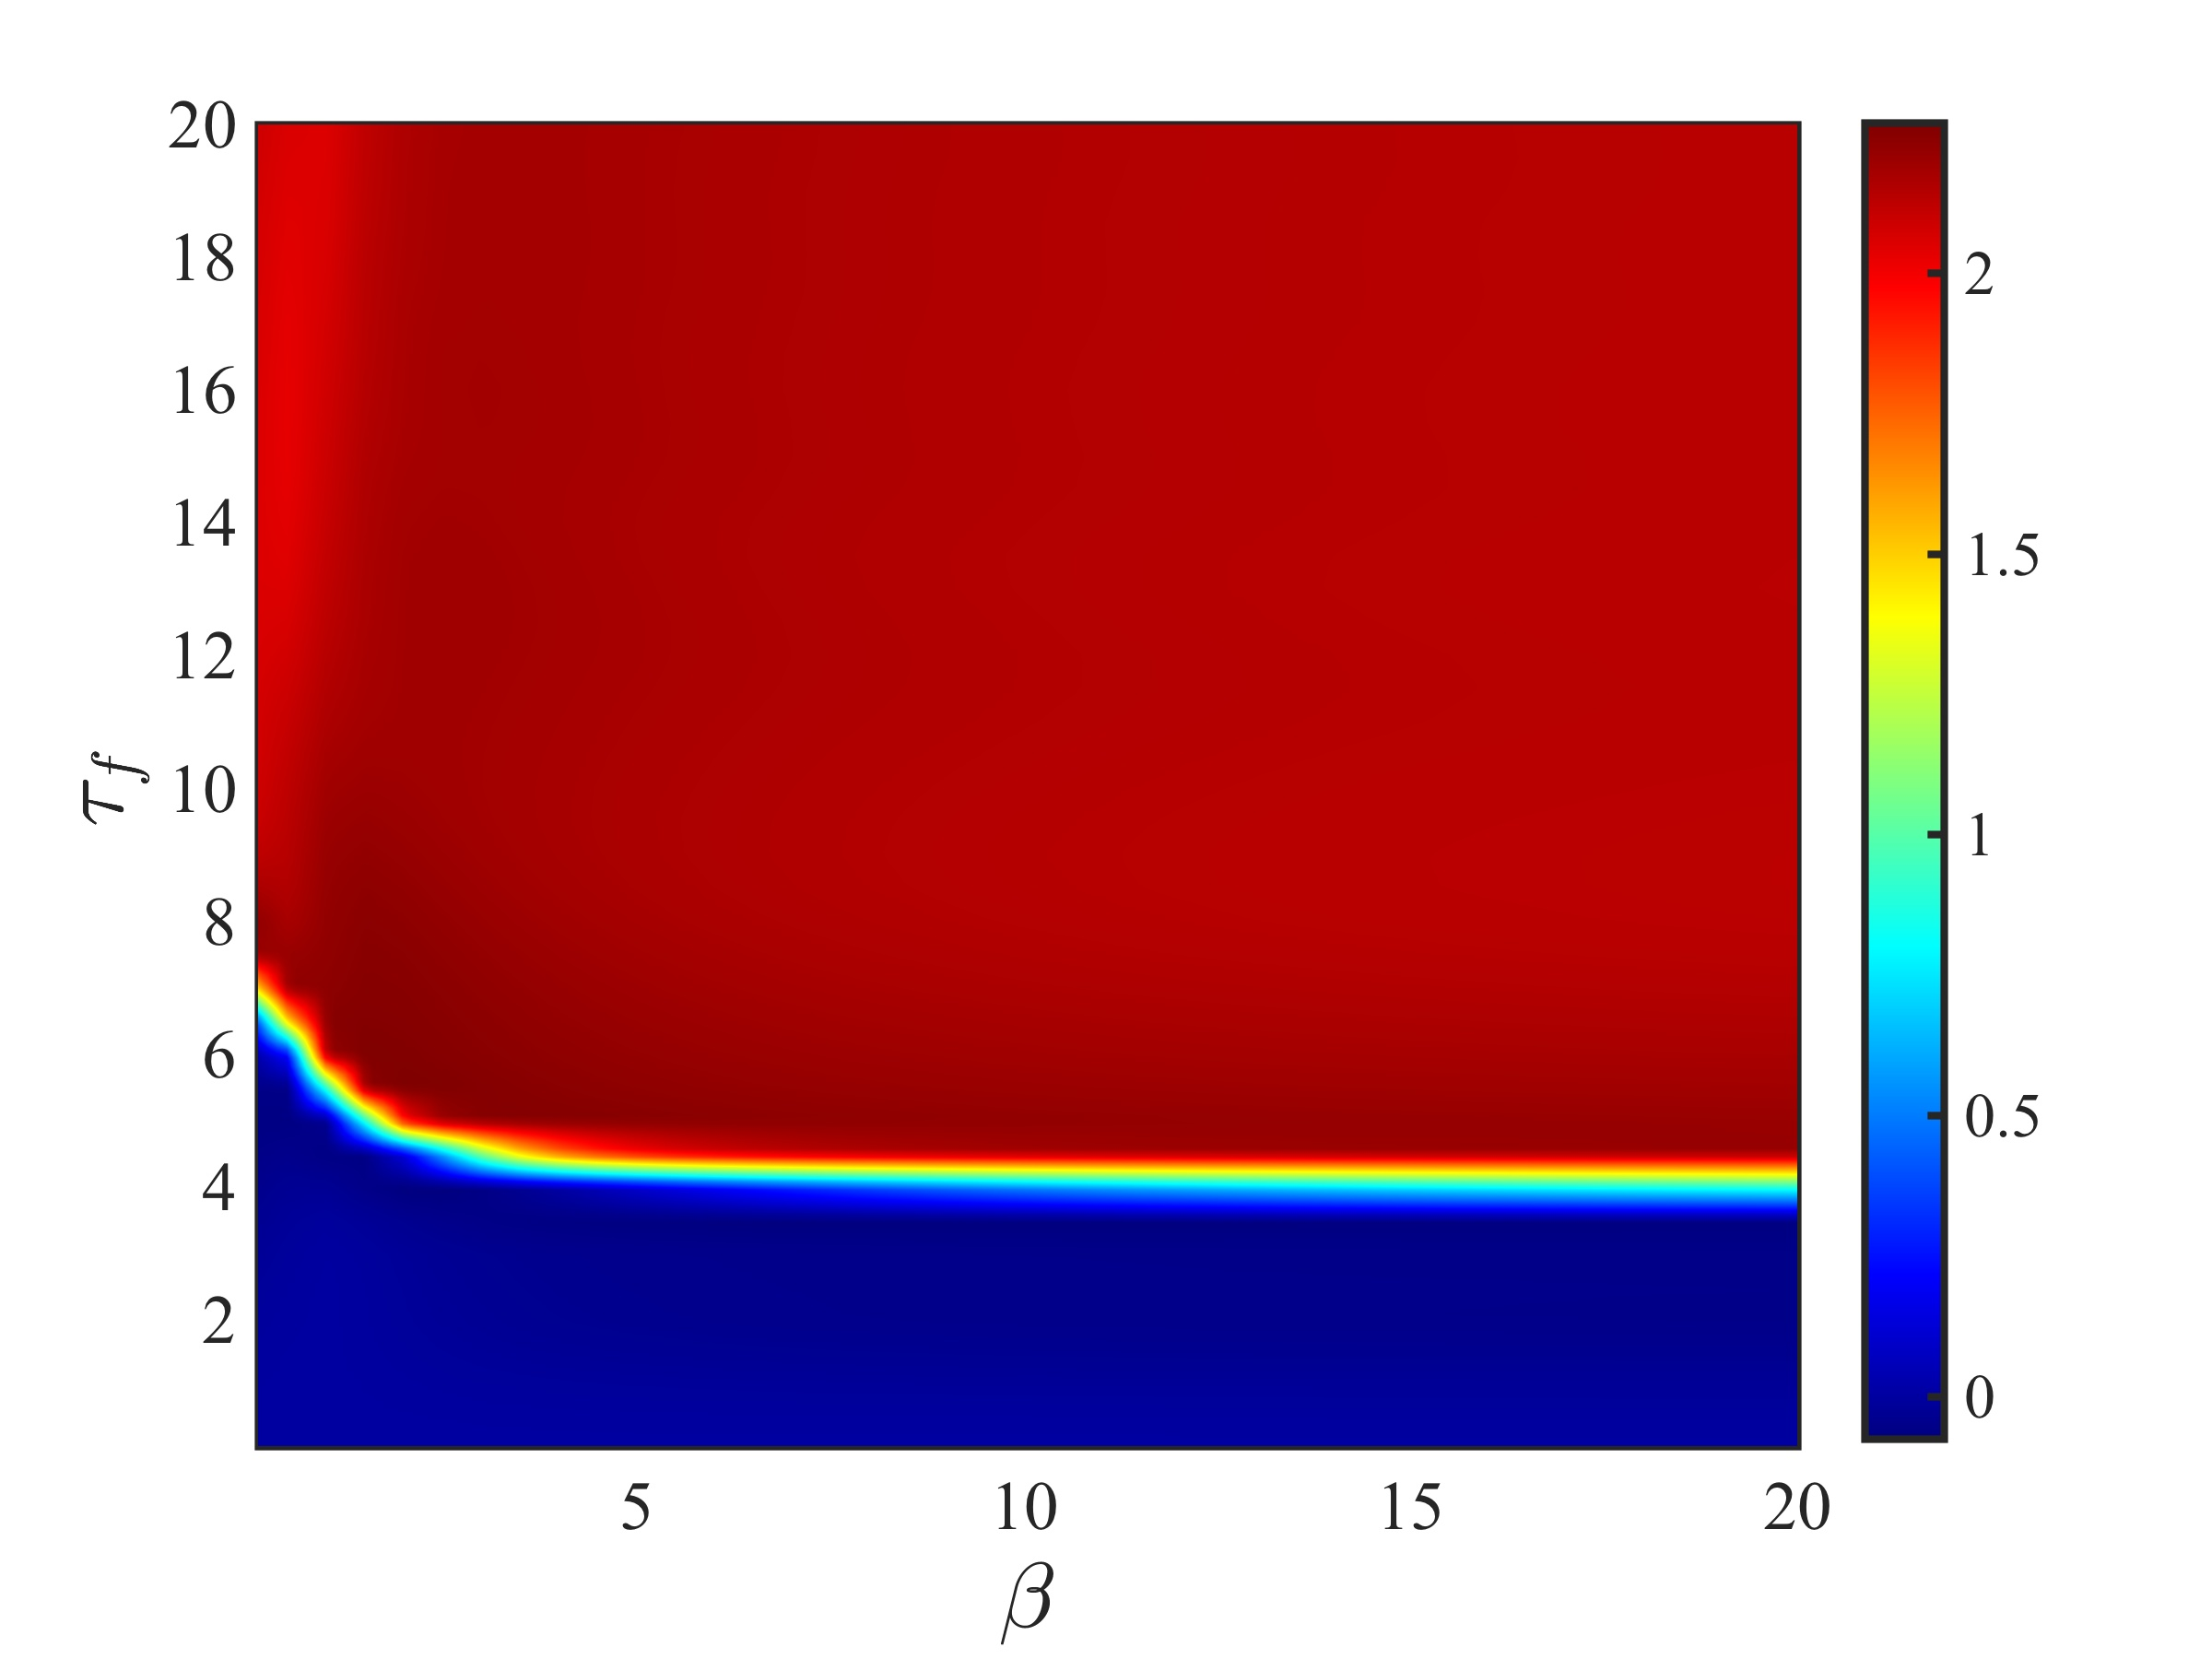
\includegraphics[width=\linewidth]{ACFatQDiff.jpg} 
\caption{} 
\end{subfigure} }
  \rule{35em}{0.5pt}
\caption[Power Ratios Inside and Outside Tweezer with $\sigma_\phi = 2$ and $h_\phi = 2$]{Power ratios as in Fig.~\ref{fig:ACSkinnyQ} but for a  tweezer with width $\sigma_\phi = 2$ and height $h_\phi = 2$.  The detuning for the system is $\Delta =  3.3830$.   Same layout as in Fig.~\ref{fig:ACSkinnyQ}.  The difference power ratio (c) defines the thresholds for tweezed CSs for all blue regions, no-CSs for all green regions, and non-tweezed CSs for all red regions.  
}
\label{fig:ACFatQ}
\end{figure}

\end{document}

\bibitem{zurek} H. Arodz, J. Dziarmaga, W.H. Zurek,
{\it Patterns of symmetry breaking}, Kluwer Academic
Publishers (Dordrech, 2003).

\bibitem{stanley} H.E. Stanley,
{\it Introduction to phase transitions and critical phenomena},
Oxford University Press (Oxford, 1971).

\bibitem{kenkre} V. M. Kenkre and D. K. Campbell
Phys. Rev. B {\bf 34}, 4959(R) (1986).

\bibitem{Boris_Gisin_Kaplan_PRE_2000}
B.V. Gisin, A. Kaplan, and B.A. Malomed,
%Spontaneous symmetry breaking and switching in planar nonlinear optical antiwaveguides.
Phys. Rev. E {\bf 62}, 2804 (2000).

\bibitem{Haelterman_OE_2006}
B. Maes, M. Solja\v{c}o\'c, J.D. Joannopoulos
P. Bienstman, R. Baets, S-P. Gorza, and M. Haelterman,
Switching through symmetry breaking in coupled nonlinear micro-cavities
Opt. Express {\bf 14}, 10678 (2006).

\bibitem{Panos_PLA_2005}
P.G. Kevrekidis, Z. Chen, B.A. Malomed, D.J. Frantzeskaki, and M.I. Weinstein.
%Spontaneous symmetry breaking in photonic lattices: Theory and experiment
Phys. Lett. A {\bf 6}, 275--280 (2005).

\bibitem{Boris_SSB_book}
B.A. Malomed,
``Spontaneous Symmetry Breaking, Self-Trapping, and Josephson Oscillations'',
%Springer Series on Atomic, Optical, and Plasma Physics,
Progress in Optical Science and Photonics, 
Springer-Verlag, Berlin, vol.~1 (2013).

\bibitem{kivshar} S.V. Suchkov, A.A. Sukhorukov, J. Huang, S.V. Dmitriev, 
C. Lee, Yu.S. Kivshar,
arXiv:1509.03378.

\bibitem{yang} V.V. Konotop, J. Yang, D.A. Zezyulin,
arXiv:1603.06826.

%\bibitem{rcg:85}

\bibitem{cartarius} H. Cartarius and G. Wunner
Phys. Rev. A {\bf 86}, 013612 (2012); see also:
A.S. Rodrigues, K. Li, V. Achilleos, P.G. Kevrekidis,
D.J. Frantzeskakis, C.M. Bender, Rom. Rep. Phys. {\bf 65}, 5 (2013).

\bibitem{rcg:88}
V. Achilleos, P.G. Kevrekidis, D.J. Frantzeskakis, and R. Carretero-Gonz\'alez.
%Dark solitons and vortices in PT-symmetric nonlinear media:
%from spontaneous symmetry breaking to nonlinear PT phase transitions.
Phys. Rev. A {\bf 86} 013808 (2012).
V. Achilleos, P.G. Kevrekidis, D.J. Frantzeskakis, and R. Carretero-Gonz\'alez,
%Solitons and their ghosts in PT-symmetric systems with defocusing nonlinearities.
Localized Excitations in Nonlinear Complex Systems, 
Nonlinear Systems and Complexity {\bf 7} 3--42 (2014).

\bibitem{XuCoen}
Y. Xu, and S. Coen,
%Experimental observation of the spontaneous breaking of the time-reversal symmetry 
%in a synchronously pumped passive Kerr resonator
Opt. Lett. \textbf{39}, 3492 (2014).

\bibitem{LL} 
L.A. Lugiato and R. Lefever, 
Spatial dissipative structures in passive optical systems. 
Phys. Rev. Lett. \textbf{58}, 2209--2211 (1987).

\bibitem{LLE} 
M. Haelterman, S. Trillo, and S. Wabnitz, 
Dissipative modulation instability in a nonlinear dispersive ring cavity. 
Opt. Commun. \textbf{91}, 401--407 (1992).

\bibitem{XuCoenRef22a}
F. Leo, S. Coen, P. Kockaert, S.-P. Gorza, Ph. Emplit, and  M.  Haelterman,  
Nat. Photon. {\bf 4}, 471--476 (2010).

\bibitem{XuCoenRef22b}
J.K.  Jang,  M. Erkintalo,  S. G.  Murdoch, and  S. Coen,
Nat. Photon. {\bf 7}, 657 (2013).

\bibitem{JuliaNCVA}
J. Rossi, R. Carretero-Gonz\'alez, and P.G. Kevrekidis,
Non-Conservative Variational Approximation for Nonlinear Schr\"odinger 
Equations.
%To appear Physica D (2016).
arXiv:1508.07040.

\bibitem{ref1}
C.R. Galley,
Phys. Rev. Lett. \textbf{110}, 174301 (2013).


\bibitem{ref4}
P.G. Kevrekidis,
%Variational method for nonconservative field theories: Formulation and 
%two PT-symmetric case examples
Phys. Rev. A {\bf 89}, 010102R (2014).

\bibitem{LLE_french_PRA}
C. Godey, I. Balakireva, A. Coillet, Y. K. Chembo,
%Stability analysis of the spatiotemporal Lugiato-Lefever model for Kerr 
%optical frequency combs in the anomalous and normal dispersion regimes.
Phy. Rev. A {\bf 89}, 063814 (2014). 

\bibitem{Galley:14}
C.R. Galley, D. Tsang, L.C. Stein,
The principle of stationary nonconservative action for classical mechanics and field theories,
arXiv:1412.3082 [math-ph].

\bibitem{tweezing} 
J.K. Jang, M. Erkintalo, S. Coen, S.G. Murdoch
Nature Communications {\bf 6}, 7370 (2015).

\bibitem{patterns}  
P. Parra-Rivas, D. Gomila, M.A. Matias, S. Coen, L. Gelens,
Phys. Rev. A {\bf 89}, 043813 (2014).




